\documentclass[preprint,letterpaper,floatfix,citeautoscript,aip,jcp]{revtex4-1}

%\documentclass[12pt]{article}
%\documentclass[letterpaper,floatfix,citeautoscript,aip,jcp]{revtex4-1}
%\documentclass[letterpaper,floatfix,citeautoscript,showkeys]{revtex4-1}
%\documentclass[twocolumn,letterpaper,floatfix,citeautoscript,jcp]{revtex4-1}
%\documentclass[twocolumn,letterpaper,floatfix,citeautoscript,aip,jcp]{revtex4-1}
%\documentclass[journal=jctc,manuscript=article]{achemso}
%\setkeys{acs}{maxauthors=30,etalmode=truncate}
%%%%%%%%%%%%%%%%%%%%%%%%%%%%%%%%%%%%%%%%%%%%%%%%%%%%%%%%%%%%%%%%%%%%%
%% Place any additional packages needed here.  Only include packages
%% which are essential, to avoid problems later.
%%%%%%%%%%%%%%%%%%%%%%%%%%%%%%%%%%%%%%%%%%%%%%%%%%%%%%%%%%%%%%%%%%%%%
\usepackage{chemformula} % Formula subscripts using \ch{}
\usepackage[T1]{fontenc} % Use modern font encodings

%%%%%%%%%%%%%%%%%%%%%%%%%%%%%%%%%%%%%%%%%%%%%%%%%%%%%%%%%%%%%%%%%%%%%
%% If issues arise when submitting your manuscript, you may want to
%% un-comment the next line.  This provides information on the
%% version of every file you have used.
%%%%%%%%%%%%%%%%%%%%%%%%%%%%%%%%%%%%%%%%%%%%%%%%%%%%%%%%%%%%%%%%%%%%%
%%\listfiles

%%%%%%%%%%%%%%%%%%%%%%%%%%%%%%%%%%%%%%%%%%%%%%%%%%%%%%%%%%%%%%%%%%%%%
%% Place any additional macros here.  Please use \newcommand* where
%% possible, and avoid layout-changing macros (which are not used
%% when typesetting).
%%%%%%%%%%%%%%%%%%%%%%%%%%%%%%%%%%%%%%%%%%%%%%%%%%%%%%%%%%%%%%%%%%%%%
% \newcommand*\mycommand[1]{\texttt{\emph{#1}}}

\usepackage{fullpage}
\usepackage{amsfonts}
\usepackage{graphicx}
\usepackage{float}
\usepackage{amsmath}
\usepackage{chemfig}
\usepackage{indentfirst}
\usepackage{longtable}
\usepackage{array}
\usepackage{cellspace}
\usepackage{palatino}
%\usepackage{breqn}
\usepackage{amssymb}
\usepackage{verbatim}
\usepackage[colorlinks=true,citecolor=blue,linkcolor=blue]{hyperref}
\usepackage{siunitx}
\usepackage{xr}
\usepackage{afterpage}

\makeatletter
\newcommand*{\addFileDependency}[1]{% argument=file name and extension
	\typeout{(#1)}
	\@addtofilelist{#1}
	\IfFileExists{#1}{}{\typeout{No file #1.}}
}
\makeatother

\newcommand*{\myexternaldocument}[1]{%
	\externaldocument{#1}%
	\addFileDependency{#1.tex}%
	\addFileDependency{#1.aux}%
}

\myexternaldocument{H:/Publications/Postdoc_3/VLE_PVT_UA_Mie_supporting_information}

%\SectionNumbersOn

% The figures are in a figures/ subdirectory.
\graphicspath{{figures/}}

%\bibliographystyle{apsrevlong}
%\bibliographystyle{apsrev}
\bibliographystyle{unsrt}

% italicized boldface for math (e.g. vectors)
\newcommand{\bfv}[1]{{\mbox{\boldmath{$#1$}}}}
% non-italicized boldface for math (e.g. matrices)
\newcommand{\bfm}[1]{{\bf #1}}          

%\newcommand{\bfm}[1]{{\mbox{\boldmath{$#1$}}}}
%\newcommand{\bfm}[1]{{\bf #1}}
\newcommand{\expect}[1]{\left \langle #1 \right \rangle} % <.> for denoting expectations over realizations of an experiment or thermal averages

\newcommand{\var}[1]{{\mathrm var}{(#1)}}
\newcommand{\x}{\bfv{x}}
\newcommand{\y}{\bfv{y}}
\newcommand{\f}{\bfv{f}}

\newcommand{\hatf}{\hat{f}}

\newcommand{\bTheta}{\bfm{\Theta}}
\newcommand{\btheta}{\bfm{\theta}}
\newcommand{\bhatf}{\bfm{\hat{f}}}
\newcommand{\Cov}[1] {\mathrm{cov}\left( #1 \right)}
\newcommand{\T}{\mathrm{T}}                                % T used in matrix transpose

%\newcommand\blfootnote[1]{%
%	\begingroup
%	\renewcommand\thefootnote{}\footnote{#1}%
%	\addtocounter{footnote}{-1}%
%	\endgroup
%}

\makeatletter
\def\blfootnote{\xdef\@thefnmark{}\@footnotetext}
\makeatother

\begin{document}

%MRS3: I think you can remove the comma before Mie.	
%RAM3: Done
\title{Bayesian inference confirms unreliable extrapolation from vapor-liquid equilibria toward high pressures of united-atom force field}
%Alternative titles: Impact of repulsive exponent on high pressure systems
%MRS1: suggestion: make the title the conclusion?  Such as ``Baysian inference shows that Mie-6 united atom force fields cannot predict vapor-liquid equilibria for alkanes?'' or ``Mie-6 united atom force fields cannot predict thermophysical properties of alkanes at high pressure''? I've had success with such straightforward titles; people know what they are getting, and get those answers when they google the question.
% Bayesian inference demonstrates limitations at high pressures of transferable, united-atom, Mie $\lambda$-6 force fields for normal and branched alkanes
% Bayesian inference analysis of transferable, united-atom, Mie $\lambda$-6 force fields for normal and branched alkanes
%Bayesian inference demonstrates limitations for predicting vapor-liquid equilibria and high pressures that united-atom, Mie $\lambda$-6 force fields for normal and branched alkanes
%Bayesian inference demonstrates that united-atom, Mie $\lambda$-6 force fields extrapolate poorly to high pressures when parameterized using vapor-liquid equilibria properties
%Bayesian inference demonstrates limitations of united-atom, Mie $\lambda$-6 force fields for predicting both vapor-liquid equilibria properties and high pressures of normal and branched alkanes
%United-atom, Mie $\lambda$-6 force fields for normal and branched alkanes extrapolate poorly to high pressures when parameterized using vapor-liquid equilibria properties
%United-atom, Mie $\lambda$-6 force fields for normal and branched alkanes perform poorly at high pressures when parameterized using vapor-liquid equilibria properties
%MRS2: performs poorly is not too specific.  ``Are inconsistent with high pressure properties''. We can wordsmith later.
%RAM2: Alright, let's revisit this.
%RAM2: This was Andrei's recommendation: Extrapolation to high pressures with united-atom, Mie $\lambda$-6 force fields parameterized using vapor-liquid equilibria properties
%RAM2: Another attempt: Dubious extrapolation to high pressures when using united-atom, Mie $\lambda$-6 force fields parameterized with vapor-liquid equilibria properties
%RAM2: Bayesian uncertainty extrapolation to high pressures when using united-atom, Mie $\lambda$-6 force fields parameterized with vapor-liquid equilibria properties
%RAM2: Bayesian inference verifies inaccurate extrapolation toward high pressures for united-atom, Mie $\lambda$-6 force fields parameterized with vapor-liquid equilibria properties
%RAM2: United-atom, Mie $\lambda$-6 force fields parameterized with vapor-liquid equilibria properties cannot be consistent with high pressure properties
%RAM2: United-atom, Mie $\lambda$-6 force fields cannot simultaneously predict vapor-liquid equilibria and high pressure properties
%RAM2: United-atom, Mie n-6 force fields cannot simultaneously predict vapor-liquid equilibria and high pressure properties
%RAM2: United-atom, Lennard-Jones n-6 force fields cannot simultaneously predict vapor-liquid equilibria and high pressure properties
%RAM2: Andrei voted in favor of this one: Unreliable extrapolation toward high pressures for united-atom, Mie $\lambda$-6 force fields parameterized with vapor-liquid equilibria properties
%RAM3: Uncertainty propagation of Mie non-bonded parameters for extrapolation from vapor-liquid equilibria toward high pressures
%RAM3: Uncertainty quantification of united-atom Mie $\lambda$-6 when extrapolating from vapor-liquid equilibria toward high pressures
%RAM3: Uncertainty propagation when extrapolating toward high pressures using united-atom Mie $\lambda$-6 force fields
%RAM3: Uncertainty quantification demonstrates that united-atom Mie $\lambda$-6 force fields cannot simultaneously predict vapor-liquid equilibria and high pressure properties
%RAM3: Uncertainty propagation of non-bonded parameters when extrapolating from vapor-liquid equilibria toward high pressures
%RAM3: Extrapolation from vapor-liquid equilibria toward high pressures using united-atom Mie force fields
%RAM3: Uncertainty propagation of Mie $\lambda$-6 non-bonded parameters verifies unreliable extrapolation from vapor-liquid equilibria toward high pressures
%RAM3: Uncertainty propagation of Mie $\lambda$-6 non-bonded parameters when extrapolating from vapor-liquid equilibria toward high pressures
%RAM3: Uncertainty propagation of Mie $\lambda$-6 non-bonded parameters confirms/demonstrates/validates/ unreliable extrapolation from vapor-liquid equilibria toward high pressures
%RAM3: Bayesian inference of Mie $\lambda$-6 non-bonded parameters confirms unreliable extrapolation from vapor-liquid equilibria toward high pressures
%RAM3: Bayesian inference of Mie $\lambda$-6 parameters confirms unreliable extrapolation from vapor-liquid equilibria toward high pressures
%RAM3: Bayesian inference confirms unreliable extrapolation from vapor-liquid equilibria toward high pressures of united-atom Mie $\lambda$-6 force field
%RAM3: Bayesian inference confirms unreliable extrapolation from vapor-liquid equilibria toward high pressures of united-atom force field


\author{Richard A. Messerly}
\email{richard.messerly@nist.gov}
\affiliation{Thermodynamics Research Center, National Institute of Standards and Technology, Boulder, Colorado, 80305}

\author{Michael R. Shirts}
\email{michael.shirts@colorado.edu}
\affiliation{Department of Chemical and Biological Engineering, University of Colorado, Boulder, Colorado, 80309}

\author{Andrei F. Kazakov}
\email{andrei.kazakov@nist.gov}
\affiliation{Thermodynamics Research Center, National Institute of Standards and Technology, Boulder, Colorado, 80305}

\keywords{Transferability, Molecular Dynamics, Molecular Simulation, Monte Carlo, Markov Chain, Bayesian Inference}%Use showkeys class option if keyword

\begin{abstract}

%MRS2: this is too much introductiony.  Can you state closer to the top what you show? Abstract should mostly focus on the conclusions (obviously, the question has to be asked). Shorten the first five sentences.
%RAM2: Alright, let me know if this is better.
%MRS3: seems good to me.
%Supplementing experimental data with molecular simulation results at extreme temperatures and pressures can extend the range  fundamental equations of state for estimating thermodynamic properties over a wide range of temperatures, pressures, and densities

Molecular simulation results at extreme temperatures and pressures can supplement experimental data when developing fundamental equations of state. Since most force fields are optimized to agree with vapor-liquid equilibria (VLE) properties, however, the reliability of the molecular simulation results depends on the validity/transferability of the force field at higher temperatures and pressures. As demonstrated in this study, although state-of-the-art united-atom Mie $\lambda$-6 potentials for normal and branched alkanes provide accurate estimates for VLE, they tend to over-predict pressures for dense supercritical fluids and compressed liquids. The physical explanation for this observation is that the repulsive barrier is too steep for the ``optimal'' united-atom Mie $\lambda$-6 potential parameterized with VLE properties. Bayesian inference confirms that no feasible combination of non-bonded parameters ($\epsilon$, $\sigma$, and $\lambda$) is capable of simultaneously predicting saturated vapor pressures, saturated liquid densities, and pressures at high temperatures and densities. This conclusion has both practical and theoretical ramifications, as more realistic non-bonded potentials may be required for accurate extrapolation to high pressures of industrial interest. 

%RAM2: A lot of failed attempts. Can clean these up once we like our abstract.

%Developing fundamental equations of state, for estimating thermodynamic properties, requires larges amounts of data over a wide range of temperatures and pressures. Recently, molecular simulation results at extreme temperatures and pressures were used to supplement experimental data when  
%
%Recently, fundamental equations of state, for estimating thermodynamic properties over a wide range of temperatures, pressures, and densities, were developed based on both experimental data and molecular simulation values can provide estimates of thermophysical properties over a wide range of temperatures and pressures. Typically, the molecular simulations are performed at extreme temperatures and pressures, where experimental data are scarce for many compounds. Since most force fields are optimized to agree with vapor-liquid equilibria properties, the reliability of the molecular simulation results depends on the validity/transferability of the force field at higher temperatures and pressures. As demonstrated in this study, although state-of-the-art united-atom Mie $\lambda$-6 potentials provide accurate estimates for vapor-liquid equilibria properties of normal and branched alkanes, they tend to over-predict pressures for dense supercritical fluids and compressed liquids. The theoretical explanation for this observation is that the repulsive barrier is too steep for the ``optimal'' united-atom Mie $\lambda$-6 potential parameterized with vapor-liquid properties. Bayesian inference confirms that no feasible combination of $\epsilon$, $\sigma$, and $\lambda$ is capable of simultaneously predicting saturated vapor pressures, saturated liquid densities, and pressures at high temperatures and densities. 

%However, the reliability of the molecular simulation results depends on the validity of the force field implemented.  . However, 
%
%Molecular simulation is a useful tool to supplement experimental data when developing fundamental equations of state for compounds with inadequate experimental data. The simulation results included in these hybrid data sets typically correspond to extreme temperatures and pressures. However, the reliability of this approach depends on the validity of the force field implemented. Most force fields are optimized to agree with vapor-liquid equilibria data. However, as demonstrated in this study, although state-of-the-art united-atom Mie $\lambda$-6 potentials provide accurate estimates for vapor-liquid equilibria properties, they tend to over-predict pressures at high temperatures and densities. The theoretical explanation for this observation is that the repulsive barrier is too steep for the ``optimal'' united-atom Mie $\lambda$-6 potential parameterized with VLE data. Bayesian inference confirms that no feasible combination of $\epsilon$, $\sigma$, and $\lambda$ is capable of simultaneously predicting saturated vapor pressures, saturated liquid densities, and pressures for dense supercritical fluids and compressed liquids.
%
% hybrid data set approach typically includes  are not available over a wide range of temperatures and pressures. However, the  reliability of this hybrid data set approach (from experiment and molecular simulation) depends on the validity of the force field implemented. 
%
%Recently, fundamental equations of state were developed based on hybrid data sets of experimental data and molecular simulation values, which are typically obtained at extreme temperatures and pressures. Developing fundamental equations of state with hybrid data sets of experimental data and molecular simulation values  requires larges amounts of data over a wide range of temperatures and pressures. Typically, the range of experimental data is limited by cost, safety, and feasibility. Molecular simulation provides an avenue for estimating thermophysical properties at extreme temperatures and pressures. The reliability of this hybrid data set approach (from experiment and molecular simulation) depends on the validity of the force field implemented. Most force fields are optimized to agree with vapor-liquid equilibria data. However, as demonstrated in this study, although state-of-the-art united-atom Mie $\lambda$-6 potentials provide accurate estimates for vapor-liquid equilibria properties, they tend to over-predict pressures at high temperatures and densities. The theoretical explanation for this observation is that the repulsive barrier is too steep for the ``optimal'' united-atom Mie $\lambda$-6 potential parameterized with VLE data. Bayesian inference confirms that no feasible combination of $\epsilon$, $\sigma$, and $\lambda$ is capable of simultaneously predicting saturated vapor pressures, saturated liquid densities, and pressures for dense supercritical fluids and compressed liquids.

%Developing fundamental equations of state requires larges amounts of data over a wide range of temperatures and pressures. Typically, the range of experimental data is limited by cost, safety, and feasibility. Molecular simulation provides an avenue for estimating thermophysical properties at extreme temperatures and pressures. The reliability of this hybrid data set approach (from experiment and molecular simulation) depends on the validity of the force field implemented. Most force fields are optimized to agree with vapor-liquid equilibria data. However, as demonstrated in this study, although state-of-the-art united-atom Mie $\lambda$-6 potentials provide accurate estimates for vapor-liquid equilibria properties, they tend to over-predict pressures at high temperatures and densities. The theoretical explanation for this observation is that the repulsive barrier is too steep for the ``optimal'' united-atom Mie $\lambda$-6 potential parameterized with VLE data. Bayesian inference confirms that no feasible combination of $\epsilon$, $\sigma$, and $\lambda$ is capable of simultaneously predicting saturated vapor pressures, saturated liquid densities, and pressures for dense supercritical fluids and compressed liquids.

\end{abstract}


\maketitle

\blfootnote{Contribution of NIST, an agency of the United States government; not subject to copyright in the United States.}


%\section*{Purpose}
%
%The aim of this study is to demonstrate, using Bayesian inference, that a UA Mie force field cannot adequately predict VLE and P$\rho$T of compressed liquids and supercritical fluids for normal and branched alkanes. For adequate prediction of VLE and compressed liquid pressures, we recommend using AUA or AA models. % or perhaps Exp-6 or extended Lennard-Jones, i.e. 12-10-8-6. %We then use simple Bayes factors (if not RJMC) to determine the optimal value of lambda for predicting compressed liquid pressures. 
%%%% RAM: Andrei and I think that we don't really need to find the best lambda value since most people would not be willing to sacrifice Pvsat just to match high pressures. Also Andrei wants to minimize the amount of effort/time required to get this paper ready.
%%%% MRS: ``since most people would not be willing to sacrifice Pvsat'': right, then just state the reasonings for not including it, that you don't think people would care.
%MRS: is it just VLE at high pressures, or everywhere?
%\section*{Outline}
%MRS: if no data on 12-10-8-6, don't recommend.
%MRS: if you say people should use AUA, then the questions is whether you need to do simulations.  It depends what the current thinking on the field is.  If AUA and Mie are thought to work, then showing that Mie doesn't is sufficient for the thesis.

%%% These were some of my thoughts before meeting with Andrei. Skip this section.

%\begin{enumerate}
%	\item Introduction
%	\item Bayesian Theory
%	\begin{enumerate}
%		\item Posterior
%		\item MCMC
%		\item RJMC
%	\end{enumerate}
%    \item MBAR-ITIC
%    \item Simulation details
%    \item Force field
%	\item Lambda (RJMC)
%	\item Transferability of CH2 sites
%	\item Transferability of CH3 sites using RJMC
%	\item Combining rules (RJMC)
%	\item Viscosity PoU
%	\item Higher pressure PoU
%\end{enumerate}
%
%Are we justified in picking just a single value for lambda? Or should we have a range of lambda values?
%Are we justified in fitting CH3 and CH2 sites simultaneously?
%Is one combining rule favored over another?
%
%I think for this paper we could focus on just a couple of these points. RJMC needs to be working for some of these. Lambda I could probably do without RJMC. Same with CH2. But others it would be necessary. 
%I basically already have the results for lambda (just ethane) and for the CH2 sites.
%
%Oh, for CH2 I could use RJMC to see if we should have a single CH2 site or if we need to have a CH2 for each. Basically I would have the same posterior (combined for all three) and I would have the model choose between the same and different. Right?
%
%So if I develop surrogate models for logp, I could perform this analysis very quickly. Then if I develop them for rhol, Psat I can change the likelihood function. For now though I am just going to use logp.
%
%Several decisions are made somewhat arbitrarily when developing force fields...
%
%I can perform a simple Bayesian inference analysis and show how the Mie potential cannot accurately predict VLE and high pressure P$\rho$T
%I could just perform this analysis for the 16-6 potential, since I already have that all done for n-alkanes
%I can show how TraPPE and Potoff perform to show the opposite trends of the 12-6 and 16-6
%Then show how the uncertainty in epsilon and sigma cannot reconcile this for the 16-6
%Then show how even a 15-6 or 14-6 potential cannot match all three properties
%
%The goal of this study is to determine if there exists a set of eps, sig, lam that accurately predicts VLE and supercritical P$\rho$T
%Specifically, we are testing whether or not the UA approach can adequately predict high pressure densities
%
%We can show how TraPPE-UA2 and/or TAMie does a better job at high pressures
%I could also simulate Exp-6

%\begin{enumerate}
%	\item Introduction
%	\item Methods I
%	\begin{enumerate}
%		\item Simulation details
%		\item Force field
%	\end{enumerate}
%	\item Case Study for alkanes
%	\item Methods II
%	\begin{enumerate}
%		\item Bayesian Analysis
%		\item Surrogate Model
%		\item Propagation of Uncertainty
%		%%%% RAM: Do we want to consider performing a Pareto front analysis to show that no set of eps, sig, lam can match all three? %%%%
%                %%%% MRS: probably would be good; I don't think it would require performing additional simulations? Also, bec clear which three properties.   
%	\end{enumerate}
%	\item Results
%	\begin{enumerate}
%		\item VLE and Compressed
%		\begin{enumerate}
%			\item Parameter uncertainties
%			\item Propagation of uncertainties
%		\end{enumerate}
%	    %\item Optimal $\lambda$ for high pressures %%% RAM: This distracts from the main purpose, that the Mie potential cannot match all three properties %%%MRS: keep it simple.
%	\end{enumerate}
%	\item Future Work
%	\item Conclusions	
%\end{enumerate}

%	\item Higher pressure PoU
%	\item Different values of lambda cannot reconcile (already done for ethane, probably need to do for other alkanes)
%	\item AUA, AUA Mie, Exp-6

%\section*{Detailed Outline}

\section{Introduction}

An accurate understanding of the relationship between pressure $(P)$, 
%MRS3: the parentheses look weird here - why is density in parentheses, when other properties are alteratives?  I would suggest just density.  Only molar volume is well defined - but why not just say density.
%RAM3: OK, I have converted everything to rho, so now I say P$\rho$T instead of PVT throughout
density ($\rho$), and temperature $(T)$ and caloric properties 
%MRS3: looks a little weird to give symbols for everything but heat capacity.
%RAM3: removed, since I could mention a lot of other derivative properties
(such as internal energy, $U$) for a given compound is essential for designing industrial chemical processes. Fundamental equations of state (FEOS), such as those based on the Helmholtz free energy, are a powerful approach for estimating $P \rho T$ behavior and caloric properties. For example, the National Institute of Standards and Technology (NIST) Reference Fluid Properties (REFPROP) currently provides FEOS for around one hundred chemical species \cite{LEMMON-RP91}. Unfortunately, most compounds do not have sufficient (reliable) experimental data covering a wide range of pressures, densities, and temperatures to develop a highly-accurate FEOS. Since FEOS are semi-empirical and have 15-30 fitting parameters, the FEOS predictions can result in large errors at temperatures and pressures that are significantly higher than those used in parameterizing the FEOS. Therefore, improvement in an FEOS at high temperatures and pressures necessitates additional data for those conditions.
% using an FEOS to extrapolate to temperatures and pressures that are significantly higher than those used in parameterizing the FEOS can result in large errors
% Most compounds do not have sufficient reliable experimental data over a wide enough region of phase space. 
%However, Thol et al. demonstrated that molecular simulation results at high temperatures and pressures can be used to supplement experimental data when developing fundamental equations of state \cite{Thol2016_siloxane}.
%Unfortunately, most compounds do not have sufficient (reliable) experimental data covering a wide range of pressures, densities, and temperatures are required to develop a highly-accurate FEOS, but are not available for most compounds.

The lack of experimental data at high temperatures and pressures, especially, is likely attributed to the inherent safety, cost, and complexity of such experiments. By contrast, molecular simulation (i.e. Monte Carlo, MC, and molecular dynamics, MD) methods at high temperatures and pressures do not suffer from any of these limitations. Therefore, in principle, molecular simulation can aid in developing FEOS \cite{Thol2016_LJ,Thol_LJTS,Rutkai2017,Lustig2015,Rutkai2015}. Although it is possible to fit an FEOS to just molecular simulation results, most studies implement hybrid data sets, i.e. from both experiment and molecular simulation \cite{Rutkai2013}.

For example, several recent studies supplement experimental data with molecular simulation results at temperatures and pressures beyond the range of available experimental temperatures and pressures \cite{Thol2016_siloxane_first,Thol2016_siloxane,Thol2017,Thol2015}. Specifically, experimental data were available for temperatures and pressures up to 580 K and 130 MPa, 590 K and 180 MPa, 450 K and 2 MPa, and 560 K and 100 MPa for hexamethyldisiloxane \cite{Thol2016_siloxane_first}, octamethylcyclotetrasiloxane \cite{Thol2016_siloxane}, ethylene oxide \cite{Thol2015}, and 1,2-dichloroethane \cite{Thol2017}, respectively. Molecular simulations were performed for these compounds at temperatures and pressures up to 1200 K and 600 MPa, 1200 K and 520 MPa, 1000 K and 700 MPa, 1000 K and 1200 MPa, respectively. The inclusion of these simulation results improved the performance of the FEOS at extreme temperatures and pressures. 

% Although it is possible to generate simulation results for the entire phase space, BLANK has shown that hybrid data sets 
% Most of the compounds studied by Refs BLANK are small compounds 
% 
%Typically, force fields are parameterized with vapor-liquid equilibria data

While previous studies have focused on small/hazardous compounds, the present study investigates normal and branched alkanes. Hydrocarbons are a fundamental feed-stock for many petrochemical processes and, therefore, large amounts of experimental data exist covering a wide range of $P \rho T$ phase space for some alkanes. For these reasons, REFPROP provides highly-accurate FEOS for several hydrocarbons, most of which are shorter-chains (less than 20 carbons) with limited branching (i.e. only methyl branches). The use of hybrid data sets is an appealing approach to develop FEOS for industrially relevant hydrocarbons with less experimental data, i.e. those with longer chain-lengths or a higher degree of branching.

% is to utilize hybrid data sets consisting of experimental data and molecular simulation results at extreme temperatures and pressures. 

%In addition, one of our aims is to determine whether the UA Mie $\lambda$-6 potential for normal and branched alkanes is reliable enough that a FEOS could be developed strictly from molecular simulation results.

The primary limitation for implementing molecular simulation at extreme temperatures and pressures is whether or not the force field, which is typically parameterized using VLE data, is reliable at those conditions.  
%MRS2: is the next clause repetitive?
%RAM2: No. I reworded it to make this more clear
%i.e. if the VLE optimal parameters are transferable to higher temperatures and pressures. 
%the VLE-optimal force field does adequately predict the homogeneous fluid region
For example, it was demonstrated that VLE-optimized force fields for small compounds, such as noble gases, hydrogen sulfide, and hydrogen chloride, do adequately represent the homogeneous fluid region \cite{Rutkai2013}. In this study, we investigate how well the traditional force fields for predicting VLE of normal and branched alkanes extrapolate to higher temperatures and pressures, i.e dense supercritical fluids and compressed liquids. This analysis is performed for four normal and four branched alkanes by comparing the simulated compressibility factor $(Z)$ with the REFPROP correlations. Note that the simulation conditions do not go beyond the range of 
%MRS3: added for clarity.
REFPROP
validity for the respective compounds, so that we can assume the REFPROP correlations are reliable.

The most accurate force fields for estimating hydrocarbon VLE properties, such as $\rho_{\rm l}^{\rm sat}$ and $P_{\rm v}^{\rm sat}$, are the Transferable Potentials for Phase Equilibria (TraPPE) \cite{TraPPE,Martin1999} (and, especially, the recent TraPPE-2 \cite{TraPPEUA2}), Errington \cite{Exp6}, fourth generation anisotropic-united-atom (AUA4) \cite{AUA4,Bourasseau2002}, Potoff \cite{Mie,Potoff_branched}, and Transferable anisotropic Mie potential (TAMie) \cite{TAMie,Weidler2016}. The TraPPE and Potoff force fields use a united-atom (UA) model while the TraPPE-2, Errington, AUA4, and TAMie force fields use an anisotropic-united-atom (AUA) model. Both a UA and AUA model group the hydrogen interactions with their neighboring carbon atom. However, the UA model assumes that the UA interaction site is that of the carbon atom, while an AUA model assumes that the AUA interaction site is shifted away from the carbon atom and towards the hydrogen atom(s). Although, in theory, an all-atom (AA) force field should yield more accurate results, from a parameterization standpoint, it is much easier to ensure that a global minimum is obtained when parameterizing UA and AUA force fields since fewer (highly correlated) parameters are optimized simultaneously. Furthermore, the reduced computational cost is an additional benefit of the UA and AUA approach.

%
%implicit hydrogens (IH) instead of explicit hydrogens (EH). An IH model does not directly compute the hydrogen interactions, rather the hydrogens are grouped with their neighboring carbon atom. The two classes of IH models are united-atom (UA) and anisotropic-united-atom (AUA). A UA model assumes that the UA interaction site is that of the carbon atom, while a AUA model assumes that the AUA interaction site is shifted away from the carbon atom and towards the hydrogen atom(s). Although, in theory, an all-atom (AA) force field should yield more accurate results, from a parameterization standpoint, it is much easier to ensure that a global minimum is obtained when optimizing UA and AUA force fields. The reduced computational cost is an additional benefit of the UA and AUA approach.
%
%Several literature UA and AUA force fields have been optimized to agree with VLE properties for normal and branched alkanes. Two of the most widely used UA based force fields are the TraPPE LJ 12-6 and Potoff Mie 16-6, while two of the most successful AUA force fields are the AUA4 LJ 12-6 and TAMie Mie 14-6. 

%In addition to the 
%%classification 
%division between
%UA and AUA force fields, the existing force fields differ in the non-bonded functional form and corresponding parameters. The TraPPE, TraPPE-2, and AUA4 force fields use a Lennard-Jones (LJ) 12-6 potential, while the Potoff and TAMie force fields use the Mie $\lambda$-6 (or generalized Lennard-Jones) potential, and the Errington force field uses the Buckingham exponential-6 (Exp-6) potential. The three-parameter Mie $\lambda$-6 and Exp-6 potentials are more flexible than the two-parameter LJ 12-6 potential as the additional adjustable parameter controls the steepness of the repulsive barrier.
%
%% have three adjustable parameters while the LJ 12-6 potential only has two parameters.
%%%RAM2: Testing out having the equation in the introduction

In addition to the 
%classification 
division between
UA and AUA force fields, the existing force fields differ in the non-bonded functional form and corresponding parameters. The TraPPE, TraPPE-2, and AUA4 force fields use a Lennard-Jones (LJ) 12-6 potential, while the Potoff and TAMie force fields use the Mie $\lambda$-6 (or generalized Lennard-Jones) potential, and the Errington force field uses the Buckingham exponential-6 (Exp-6) potential. 
%MRS3: should mention somewhere that it's a variant of the Lennard-Jones n-m.
%RAM3: Found in the paragraph that follows
The Mie $\lambda$-6 potential is \cite{Herdes2015}:
\begin{equation} \label{eq:Mie}
u^{\rm vdw}(\epsilon,\sigma,\lambda;r) = \left(\frac{\lambda}{\lambda - 6}\right)\left(\frac{\lambda}{6}\right)^{\frac{6}{\lambda - 6}} \epsilon \left[\left(\frac{\sigma}{r}\right)^\lambda - \left(\frac{\sigma}{r}\right)^6\right]
\end{equation} 
where $u^{\rm vdw}$ is the van der Waals interaction, $\sigma$ is the distance $(r)$ where $u^{\rm vdw} = 0$, $-\epsilon$ is the energy of the potential at the minimum $\left(\text{i.e. }u^{\rm vdw} = -\epsilon \text{ and } \frac{\partial u^{\rm vdw}}{\partial r} = 0 \text{ for } r=r_{\rm min} \right)$, and $\lambda$ is the repulsive exponent. 

The Buckingham exponential-6 model is \cite{Exp6}:
\begin{equation} \label{eq:Buckingham}
u^{\rm vdw}(\epsilon,r_{\rm min},\alpha;r) = 
\begin{cases}
\frac{\epsilon}{1-\frac{6}{\alpha}} \left[\frac{6}{\alpha} \exp\left(\alpha\left[1-\frac{r}{r_{\rm min}}\right]\right) - \left(\frac{r_{\rm min}}{r}\right)^6\right] & \text{for}\ r>r_{\rm max} \\
\infty           & \text{for}\ r<r_{\rm max}
\end{cases}
\end{equation}
where $u^{\rm vdw}$, $\epsilon$, and $r$ are the same as in Equation \ref{eq:Mie}, $r_{\rm min}$ is the distance that corresponds to the minimum in the potential (i.e $u^{\rm vdw}(r_{\rm min})=-\epsilon$), $\alpha$ is a Buckingham exponential-6 parameter, and $r_{\rm max}$ is the smallest positive value for which $\frac{du^{\rm vdw}}{dr}=0$.

The three-parameter Mie $\lambda$-6 and Exp-6 potentials are more flexible than the two-parameter LJ 12-6 potential as an additional adjustable parameter controls the steepness of the repulsive barrier. Note that the Mie $\lambda$-6 potential reduces to the LJ 12-6 potential for $\lambda = 12$. Therefore, the LJ 12-6 potential can be considered a special subclass of the Mie $\lambda$-6 potential. 

% have three adjustable parameters while the LJ 12-6 potential only has two parameters.

Previous work demonstrated that the UA LJ 12-6 potential cannot adequately estimate both $\rho_{\rm l}^{\rm sat}$ and $P_{\rm v}^{\rm sat}$ for \textit{n}-alkanes \cite{Pareto_LJPQ,Mess4}. For this reason, the TraPPE-UA force field was primarily developed to agree with $\rho_{\rm l}^{\rm sat}$ (and the critical temperature, $T_{\rm c}$) \cite{TraPPE}. By contrast, accurate prediction of both $\rho_{\rm l}^{\rm sat}$ and $P_{\rm v}^{\rm sat}$ over a wide temperature range is possible by varying the repulsive exponent of the LJ potential (i.e. the Mie $\lambda$-6 potential). It is important to mention that, although an attractive exponent of 6 has a strong theoretical basis, $\lambda = 12$ (LJ 12-6) is a historical artifact that was chosen primarily for computational purposes \cite{Allen1987}.

Typically, when parameterized to VLE data, the optimal value of $\lambda$ is greater than 12 with a corresponding increase in the well depth $(\epsilon)$. Specifically, for most hydrocarbons, the Potoff UA force field \cite{Mie,Potoff_branched} uses $\lambda = 16$ while the TAMie force field \cite{TAMie} uses $\lambda = 14$. Gordon also demonstrated that reliable viscosities can be obtained from a UA Mie $\lambda$-6 model for \textit{n}-alkanes by using $\lambda = 14$ and $\lambda = 20$ for the CH$_3$ and CH$_2$ sites, respectively (note the subtle difference in how Gordon defines the Mie $\lambda$-6 potential, a.k.a. ``mod-n-6'') \cite{Gordon2006}. 
%MRS2: don't make this a parenthetical. Full sentences generally shouldn't be.
%RAM2: Alright, I admit that I use this tactic too often.
However, it is important to note that Gordon and Galli{\'e}ro et al. report $\lambda$ values of 11 and 10, respectively, for UA methane when optimized with viscosity data \cite{Gordon2006,Galliero2005}.

%(It is interesting to note that, for UA methane, Gordon and Galli{\'e}ro et al. reported that the optimal $\lambda$ to reproduce viscosity data is less than 12 (11 and 10, respectively) \cite{Gordon2006,Galliero2005}.)

%(It is interesting to note that Gordon and Galli{\'e}ro et al. report $\lambda$ values of 11 and 10, respectively, for UA methane when optimized with viscosity data \cite{Gordon2006,Galliero2005}.)

There are some theoretical concerns that increasing the repulsive exponent might have some undesirable consequences, especially at high pressures, where 
%close range interactions will become more prevalent 
particles will spend more time with very short  pairwise distances
than at VLE conditions. For example, References \citenum{Rowley1999,Rowley2001,Hayes2004} demonstrate that neither an all-atom LJ 12-6 or an all-atom LJ 9-6 is adequate to reproduce high-level \textit{ab initio} calculations of \textit{n}-alkanes ranging from methane to \textit{n}-butane. 
%MRS2: can you be more precise?  Which ab initio energies?  The entire pairwise curve? cluster energies?
%RAM2: These are single-point energies computed at several different configurations and center-of-mass distances
The studies of Rowley et al. suggest a modified-Morse potential is necessary for accurate representation of \textit{ab initio} dimer energies \cite{Rowley1999,Rowley2001}. Hayes et al. confirms these results while also emphasizing that the short-range repulsive forces, which are most important when computing high pressures in molecular simulation, are poorly represented with an AA LJ 12-6 or an AA LJ 9-6 model \cite{Hayes2004}. Specifically, the LJ 12-6 potential is too steep, and only slight improvement in the repulsive region is observed for the LJ 9-6 potential. %MRS2: suggest removing parenthetical, as well as as a brief aside; If you talk about Morse, then talking about Buckingham as well. 
%RAM2: Done
%MRS3: ``it is interesting that X'' isn't a good way to state something, because it doesn't say what was interesting about it.  Did Hayes say it is too shallow or something else?
%RAM3: They said ``this indicated deficiencies of the exp-6 function in its description of repulsion. So not much to work with. The ``this'' referred to the large errors in the repulsive region of their fit.
Note that Hayes et al. also highlights deficiencies in the repulsive region for the Buckingham exponential-6 potential. 
%MRS2: Suggest actually writing out the general Mie equation earlier in the intro,  just for concreteness in the introduction, then can refer back to it when defining specific potentials.  Couldn't hurt to put morse and buckingham, but not vital, since you don't really explore it.  
%RAM2: I thought about this too, but it seemed strange to have an equation in the introduction.

Recently, Kulakova et al. used Bayesian inference to conclude that experimental data for argon, specifically the liquid and vapor radial distribution functions at varying temperatures and densities, support $\lambda$ values between 6 and 10, while argon dimer \textit{ab initio} energies support $\lambda$ values between 12 and 14 \cite{Kulakova2017}. They suggest that these larger values of $\lambda$ should not be used for liquid phase simulations. By contrast, two other studies of noble gases, including argon, support $\lambda \ge 12$ \cite{Galliero2005,Mick_Mie}. Specifically, Mick et al. reports a 13-6 potential for argon, while Galli{\'e}ro et al. states that the 12-6 potential is superior for argon than the 10-6, 14-6, 16-6, 18-6, and 20-6 potentials. The likely explanation for this discrepancy is the choice of experimental data. The conclusions from Kulakova et al. are based on the radial distribution function, while Galli{\'e}ro et al. used viscosity and pressure, and Mick et al. utilized VLE data.

Structural properties, such as the radial distribution function, and \textit{ab initio} calculations provide considerable insight into the true repulsive barrier \cite{Kulakova2017,Galliero2005}. However, the ``correct'' value of $\lambda$ does not guarantee adequate prediction of VLE and/or $P \rho T$ behavior. This is primarily because the Mie $\lambda$-6 potential is only an approximation to the real potential and, thus, it is not flexible enough to agree with both the repulsive and attractive regions. Instead, only the region that is most sensitive to the target experimental data will be adequately represented, which for VLE data is typically the 
%MRS3: I think no hyphen.
%RAM3: Done
effective size, depth of the energy minimum, and the dispersive tail. Furthermore, the ``optimal'' $\lambda$ is not necessarily the ``true'' $\lambda$ because force fields use effective parameter sets that account for assumptions, such as pair-wise additivity (i.e. excluding three-, four-, etc. body interactions) or the lack of explicit hydrogens. For example, a UA Mie $\lambda$-6 potential is simply not capable of predicting VLE properties of ethane for $\lambda < 12$ (see Figures 1-2 of Reference \citenum{Mie}), despite theoretical evidence that the repulsive barrier should be softer than $\lambda = 12$.

%This is primarily because force fields use ``effective'' parameter sets that try to account for assumptions, such as pair-wise additivity (i.e. excluding three-, four-, etc. body interactions) or the lack of explicit hydrogens. Furthermore, because the Mie $\lambda$-6 potential is only an approximation to the real potential, it is not flexible enough to agree with both the repulsive and attractive region. Instead, only the regions that impact the target experimental data are most accurate, which for VLE data is typically the effective-size, depth of the energy minimum, and the dispersive tail.


%the importance of the forces, which are used to compute pressures in molecular simulation. Hayes et al. shows that the short-range repulsive forces, which are most important at high pressures,

%While these results are for an all-atom model, it gives to reason that deficiencies would be even more pronounced for a more coarse united-atom model, especially when using a harder potential, i.e. $\lambda > 12$. 

%Although it is difficult to know if the results for noble gases and all-atom alkane models are applicable to united-atom interaction sites for alkanes, 


%several studies suggest the need for $\lambda$ values greater than 12 to match VLE data \cite{Gordon2006,Mie,Potoff_branched,TAMie}. 

The purpose of this study is to determine whether or not the UA Mie $\lambda$-6 model is adequate for predicting \textit{both} VLE and 
%MRS3: not sure what you mean by P$\rho$T at high temperatures.  Pressure as a function of volume and T? Compressibility?  Its a vague term (and used a lot throughout).
%RAM3: Yeah I could just say Z. Sometimes P$\rho$T behavior is more inclusive, but in this case where I specify high temperature and pressure I should probably say $Z$ instead
$P \rho T$ at high temperatures and pressures for alkanes. Although it is difficult to know if the theoretical studies discussed previously for noble gases and all-atom \textit{n}-alkane models are applicable to UA models for normal and branched alkanes, the working hypothesis based on the literature is that a UA Mie $\lambda$-6 potential parameterized with VLE data is too repulsive and, thus, performs poorly at high pressures. 
%MRS2: above: be specific as to what evidence from above you are using to reach this conclusion so the reader knows.
%RAM2: OK, hopefully this is better
This assessment is of practical engineering importance for deciding whether or not UA Mie $\lambda$-6 force fields should be used when developing fundamental equations of state for alkanes based on hybrid data sets.

%By demonstrating the inadequacy of the UA Mie $\lambda$-6 potential at high pressures, we support the theoretical understanding that t

% since Hayes et al. demonstrated that the AA LJ 12-6 potential was too steep, it gives to reason that    


%
%It is important to remember that Kulakova et al. only investigated a truly single-site molecule, while in this study we are interested in united-atom models.
%
%For this and other theoretical reasons, there is some concern that increasing the repulsive exponent might have some undesirable consequences, especially at high pressures, where close range interactions will become more prevalent than at vapor-liquid equilibria.  

%Gordon reports that, for methane, an 11-6 potential is best for reproducing viscosity data, while he reports a 14-6 and 20-6 potential for CH$_3$ and CH$_2$ sites (note the subtle difference in how Gordon defines the Mie $\lambda$-6 potential, a.k.a. ``mod-n-6'').

% which will  The studies of Rowley et al. and Hayes et al. conclude that a Morse potential is necessary for   The results from Rowley et al. and Hayes et al. suggest that a Morse function is needed 

%All-atom

%The purpose of this study is to determine whether or not the UA Mie $\lambda$-6 potential is adequate for predicting both VLE and $P \rho T$ at higher temperatures and pressures.

%there is some concern that increasing the repulsive exponent might have some undesirable consequences, especially at high pressures, where close range interactions will become more prevalent than at vapor-liquid equilibria. The purpose of this study is to determine whether or not the UA Mie $\lambda$-6 potential is adequate for predicting both VLE and $P \rho T$ at higher temperatures and pressures. 

% < 12$, specifically $\lambda \approx 6.5$, while $\lambda = 12$-$14$ reproduced quantum dimer energies most accurately.  results suggest that $\lambda > 12$ $6 < \lambda < 12$  that $\lambda < 12$
%MRS2: Suggest ``for this study'' rather than ``for this manuscript''. May need to reorganize sections into methods, results, etc depending on the journal, rather than numbered sections
%RAM2: Done
The outline for this study is the following. Section \ref{Methods I} discusses the simulation and force field details. Section \ref{Case Study} is a case study for normal and branched alkanes using the existing force fields developed based on VLE properties. Section \ref{Methods II} explains how Bayesian inference is employed to investigate the adequacy of the UA Mie $\lambda$-6 potential. Section \ref{Results} presents the results from the Bayesian analysis with recommendations and limitations in Section \ref{Discussion}. Section \ref{Conclusions} reports the primary conclusions of this study.

%when properly optimized, the Mie potential can accurately predict both $\rho_{\rm l}^{\rm sat}$ and $P_{\rm v}^{\rm sat}$ over a wide temperature range. This improvement  However, there is some concern that increasing the repulsive exponent (in this case, from 12 to 16) might have some undesirable consequences, especially at high pressures, where close range interactions will become more significant. The purpose of this study is to determine whether or not the UA Mie potential is 
%
%are reliable at high temperatures and pressure
%
%Several 
%
%Although, in theory, an all-atom (AA) force field would be more reliable than a UA and AUA force field, from a parameterization standpoint, it is much easier to ensure that a global minimum is obtained when optimizing UA and AUA force fields.
%
%The most reliable hydrocarbon force fields for estimating VLE properties (i.e. $\rho_{\rm l}^{\rm sat}$ and $P_{\rm v}^{\rm sat}$) are based on the united-atom (UA) assumption, where hydrogen interactions are grouped with their neighboring carbon atom, or the anisotropic-united-atom (AUA) model, where the hydrogens  force fields are typically considered 
%
%Hydrocarbons 
%
%Several force fields in the literature have been optimized to agree with VLE properties for normal and branched alkanes. Two of the most widely used united-atom based force fields are the TraPPE LJ 12-6 and Potoff Mie 16-6.
%
%It has been demonstrated that the united-atom LJ 12-6 potential cannot adequately estimate both $\rho_{\rm l}^{\rm sat}$ and $P_{\rm v}^{\rm sat}$. By contrast, when properly optimized, the Mie 16-6 potential can accurately predict both $\rho_{\rm l}^{\rm sat}$ and $P_{\rm v}^{\rm sat}$ over a wide temperature range. However, there is some concern that increasing the repulsive exponent (in this case, from 12 to 16) might have some undesirable consequences, especially at high pressures, where close range interactions will become more significant.

%When sufficient experimental data are available over a wide range of pressures, densities, and temperatures highly accurate fundamental equations-of-state (FEOS) are possible. However, for most compounds the data are scarce and do not cover a wide enough region of phase space. The National Institute of Standards and Technology (NIST) currently provides on the order of one hundred fundamental equations-of-state (FEOS) for chemical species that have sufficient characterization.  

%Large amounts of data are required
%
%P$\rho$T data are important
%
%
% requires 
%The ability to predict both vapor-liquid equilibria and pressure, volume, temperature $(P$\rho$T)$
%
% The reliability of 

%\begin{enumerate}
%	\item Developing reliable fundamental equations of state (REFPROP) is an arduous task that relies on having high accuracy data over a wide range of state points
%	\item Reliable predictions for high pressure systems are important for many industrial applications
%	\item Recently, molecular simulation results have supplemented experimental data when developing fundamental equations of state
%%MRS: I wouldn't inlcude on the fluid properties simulation challenge.  It might the reason you are interested, but it isn't the reason the readers would be interested. 
%%	\item In addition, the 10th Industrial Fluid Properties Simulation Challenge is to predict the viscosities at high pressures of a highly branched alkane. Reliable P$\rho$T predictions are essential for this challenge.
%	\item The UA Mie potential has received significant attention for its ability to predict VLE without requiring an all-atom representation
%	\item However, the impact that modifying the repulsive exponent has on the higher pressure states has not been tested
%%MRS: you didn't say earlier the importance was properties at supercritical pressures as well.  You did say compressed; make languate consistent throughout.
%	\item The purpose of this study is to perform a rigorous Bayesian analysis as to the adequacy of a UA Mie potential for predicting both VLE and compressed liquid/supercritical pressures
%\end{enumerate}

\section{Methods I} \label{Methods I}

\subsection{Simulation Details}
%MRS2: provide justification for number and choice of molecules.
%RAM2: Done
Four normal and four branched alkanes of varying chain-length and degree of branching are simulated in this study. Specifically, we simulate ethane, propane, \textit{n}-butane, \textit{n}-octane, isobutane (2-methylpropane), isohexane (2-methylpentane), isooctane (2,2,4-trimethylpentane), and neopentane (2,2-dimethylpropane). These compounds were chosen to represent a diverse set of the normal and branched alkanes available in REFPROP \cite{LEMMON-RP91}.

%MRS2: might want to be explicit there are no charges (helps to remind people)  
%RAM2: Done
%MRS2: how is the vdw truncated?  I would suggest distributing the input files in supporting information as part of best practices.
%RAM2: How specific do you think I should be for discussing vdw cut-offs?
%RAM2: I plan on including input files.
Simulations for this study are performed in the $NVT$ ensemble (constant number of molecules, $N$, constant volume, $V$, and constant temperature, $T$) using GROMACS version 2018 \cite{GROMACS_2018}. Each simulation uses the Velocity Verlet integrator with a 2 fs time-step, 1.4 nm cut-off 
%MRS3: shifted, switched? abrupt? abrupt is not very physical.
%RAM3: But the abrupt cut-off is how the TraPPE, Potoff, etc. force fields were parameterized. A shifted or switched would dramatically change the results
for non-bonded interactions with tail corrections for energy and pressure, Nos{\'e}-Hoover thermostat with a time constant of 1 ps, and fixed bond-lengths 
%MRS3: deleted.
%are 
constrained using LINCS with a LINCS-order of eight. Coulombic interactions are not computed as none of the force fields require partial charges for the compounds studied. The equilibration time is 0.1 ns for ethane and propane, 0.2 ns for \textit{n}-butane, and 0.5 ns for all other compounds. The production time is 1 ns for ethane, 2 ns for propane and \textit{n}-butane, and 4 ns for all other compounds. Replicate simulations are performed for \textit{n}-octane to validate that a single MD run of this length agrees with the average of several replicates, to within the combined uncertainty. A system size of 400 molecules is used for ethane, propane, and \textit{n}-butane, while all other compounds use 800 molecules. 
%MRS3: I would provide the actual ascii files, not put them in a PDF.  That makes them very hard to use.
%RAM3: That was my plan. I should not have included a section for this.
Example input files are provided as Supporting Information.

%MRS2: these are for ITIC, correct? State that, so it's not vague wat the purpose of these are.
%RAM2: Done
The specific state points for each compound studied are depicted in Figure \ref{fig:simulation_conditions} (for tabulated values, see Section \ref{Simulation Set-Up} of Supporting Information). 
These state points correspond to the recommended conditions for the isothermal isochoric integration (ITIC) algorithm discussed in Section \ref{Methods II} \cite{Mostafa_Diss,Postdoc_1,Mostafa2018}. 
Simulations are performed along a supercritical isotherm (with a reduced temperature, $T_{\rm r} \approx 1.2$) and five saturated liquid density isochores. Nine densities are simulated along the supercritical isotherm $(T^{\rm IT})$ with five densities being the same as the isochore densities $(\rho^{\rm IC})$. Two additional temperatures are simulated along each isochore, with one being the REFPROP saturation temperature $(T^{\rm sat})$ while the inverse of the second isochore temperature is the average of $1/T^{\rm IT}$ and $1/T^{\rm sat}$. Thus, a total of 19 simulations are performed for each compound and force field.

%Tabulated values for the state points of each compound are provided in Section \ref{Simulation Set-Up} of Supporting Information.

\begin{figure}[htb!]
	\centering
	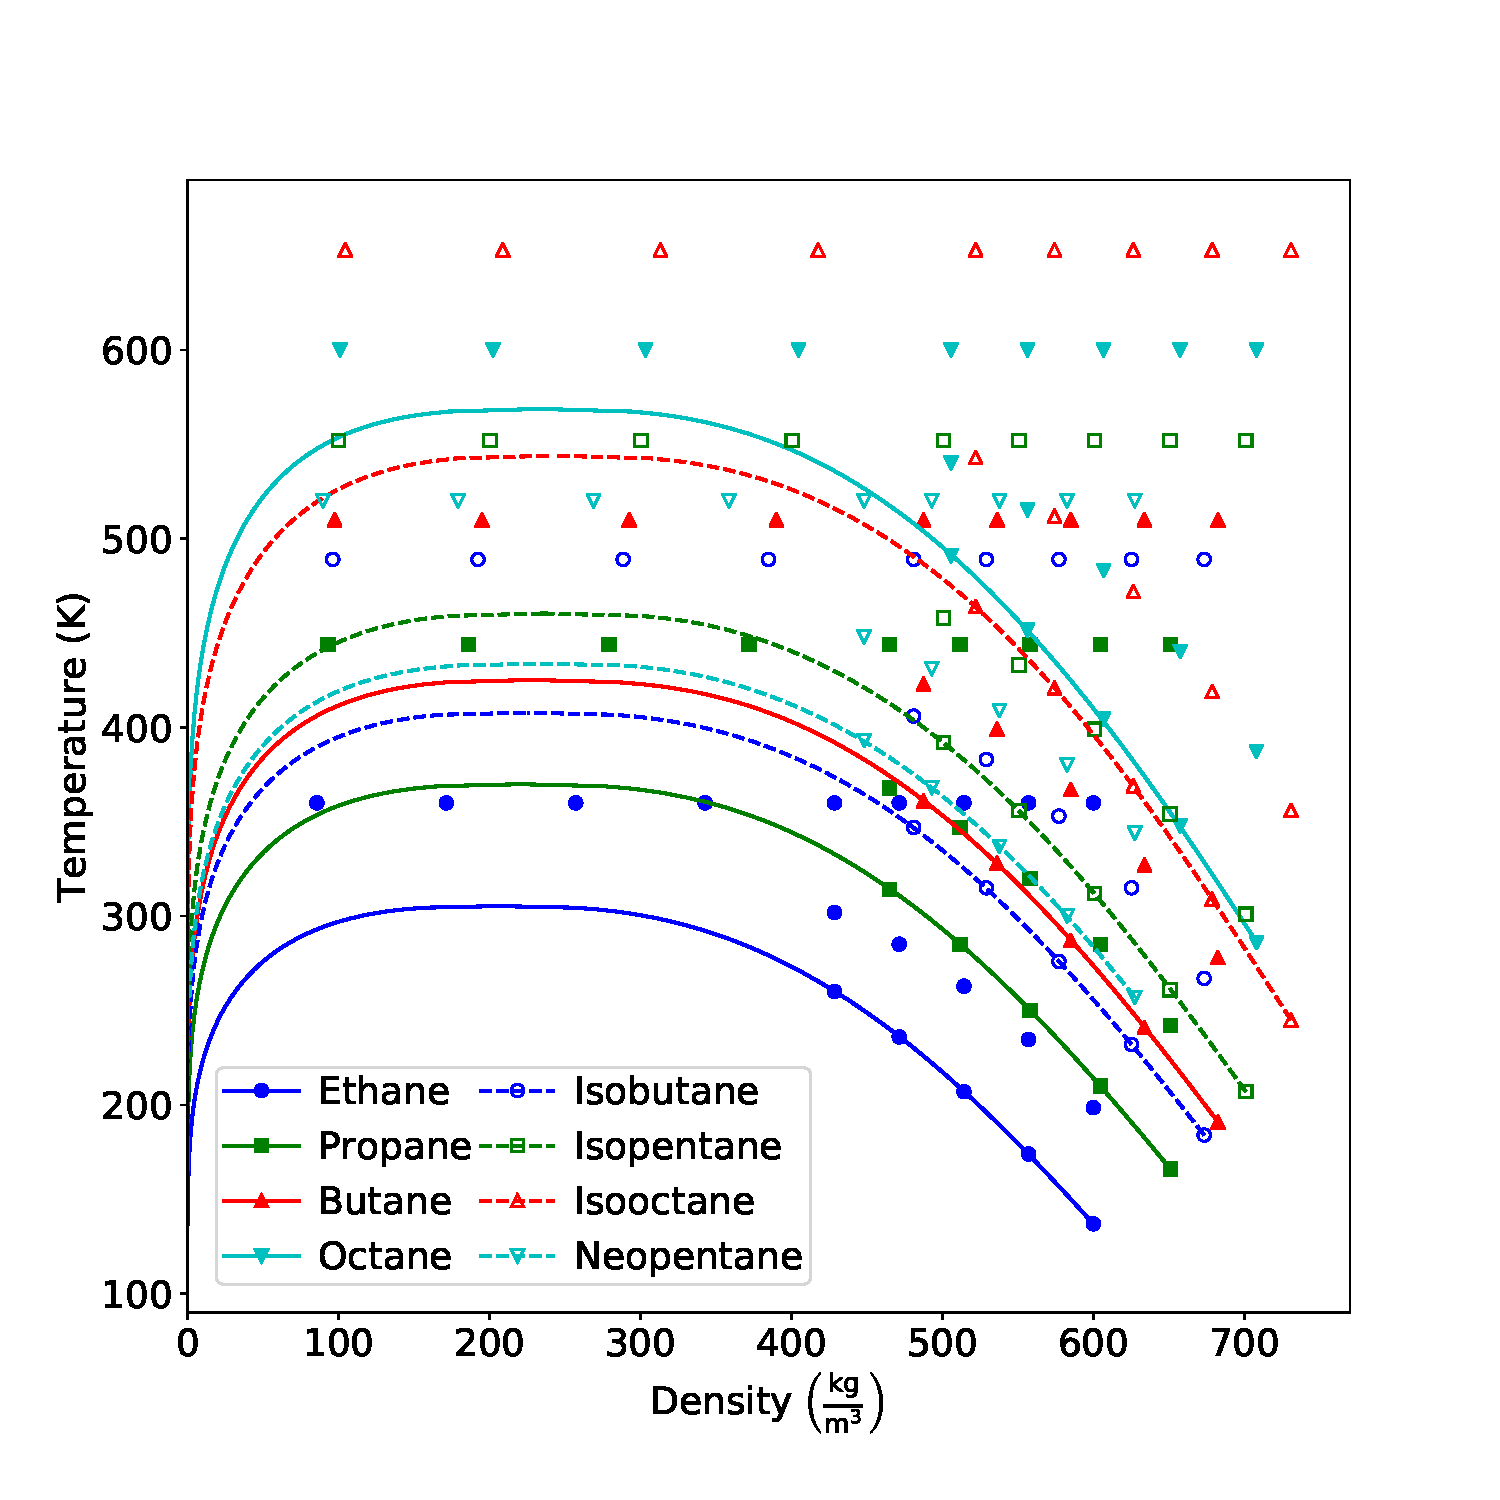
\includegraphics[width=3.2in]{simulation_conditions}
	\caption{State points simulated for each compound studied. A total of 19 simulations are performed: nine densities along the supercritical isotherm and two temperatures along five liquid density isochores. Filled symbols and solid lines correspond to \textit{n}-alkanes, while empty symbols and dashed lines correspond to branched alkanes. The REFPROP saturation curve for each compound is included as a reference.}
	\label{fig:simulation_conditions}
\end{figure}

%The state points depicted in Figure \ref{fig:simulation_conditions} correspond to the recommended conditions for the isothermal isochoric integration (ITIC) algorithm \cite{Mostafa_Diss,Postdoc_1}. 
%ITIC converts the departure internal energies $(U^{\rm dep})$ and compressibility factors $(Z)$ obtained at the 19 state points to saturated VLE properties, namely, $\rho_{\rm l}^{\rm sat}$ and $P_{\rm v}^{\rm sat}$.
%The 
%%fundamental 
%equations for ITIC are: 
%\begin{equation} \label{ITIC A}
%\frac{A^{\rm dep}}{R_{\rm g}T^{\rm sat}} = \int_{0}^{\rho_{\rm l}^{\rm sat}}\frac{Z-1}{\rho} \partial \rho |_{T = T^{\rm IT}} + \int_{T^{\rm IT}}^{T^{\rm sat}}U^{\rm dep}\partial\left(\frac{1}{R_{\rm g}T}\right)|_{\rho=\rho_{\rm l}^{\rm sat}}
%\end{equation}
%\begin{equation} \label{ITIC rhov}
%\rho_{\rm v}^{\rm sat} \approx \rho_{\rm l}^{\rm sat} \exp \left( \frac{A^{\rm dep}}{R_{\rm g}T^{\rm sat}} + Z_{\rm l}^{\rm sat} - 1 - 2 B_2 \rho_{\rm v}^{\rm sat} - 1.5 B_3 (\rho_{\rm v}^{\rm sat})^2 \right)
%\end{equation}
%\begin{equation} \label{ITIC Pv}
%P_{\rm v}^{\rm sat} \approx \left(1 + B_2 \rho_{\rm v}^{\rm sat} + B_3 (\rho_{\rm v}^{\rm sat})^2\right)\rho_{\rm v}^{\rm sat} R_{\rm g}T^{\rm sat}
%\end{equation}
%\begin{equation} \label{ITIC Zl}
%Z_{\rm l}^{\rm sat} = \frac{P_{\rm v}^{\rm sat}}{\rho_{\rm l}^{\rm sat} R_{\rm g} T^{\rm sat}}
%\end{equation}
%where $A^{\rm dep} \equiv A-A^{\rm ig}$ is the Helmholtz free energy departure from ideal gas for temperature $(T)$ equal to the saturation temperature $(T^{\rm sat})$ and density $(\rho)$ equal to the saturated liquid density $(\rho_{\rm l}^{\rm sat})$, $U^{\rm dep} \equiv U-U^{\rm ig}$ is the internal energy departure, $Z_{\rm l}^{\rm sat}$ is the saturated liquid compressibility factor $(Z)$, $B_2$ is the second virial coefficient, $B_3$ is the third virial coefficient, $T^{\rm IT}$ is the isothermal temperature, and $R_{\rm g}$ is the universal gas constant. For details regarding the implementation of ITIC, see Reference \citenum{Postdoc_1}. As discussed in our previous work \cite{Postdoc_1}, the $B_2$ and $B_3$ values found in Equations \ref{ITIC rhov}-\ref{ITIC Pv} are calculated using REFPROP correlations \citenum{LEMMON-RP91}. The use of REFPROP correlations introduces a small bias in the resulting $\rho_{\rm l}^{\rm sat}$ and $P_{\rm v}^{\rm sat}$, which is accounted for in Section \ref{Bayesian Analysis}.   

%\begin{enumerate}
%	\item The compounds simulated in this study are ethane, propane, \textit{n}-butane, \textit{n}-octane, isobutane, isopentane, isohexane, isooctane, and neopentane
%	\item These compounds were selected as a sample set for 2,2,4-trimethylhexane, the compound studied in the 10th Industrial Fluid Properties Simulation Challenge
%	\item We perform NVT simulations in GROMACS along a supercritical isotherm and five isochores that correspond to saturated liquid densities
%	\item We use ITIC to convert the Udep and Z values obtained from the NVT simulations to rholsat and Pvsat
%	\item The specific state points are depicted in Figure, tabulated values are provided in supporting information
%%MRS: probably should give main settings in the text. 
%	\item The GROMACS settings are provided in supporting information
%\end{enumerate}

\subsection{Force field} \label{Force Field}

A united-atom (UA) or anisotropic-united-atom (AUA) representation is used for each compound studied. The UA and AUA groups required for normal and branched alkanes are sp$^3$ hybridized CH$_3$, CH$_2$, CH, and C sites. For most literature models, a single (transferable) parameter set is assigned for each interaction site. However, two exceptions exist for the force fields studied. First, TAMie implements a different set of CH$_3$ parameters for ethane. Second, Potoff reports a ``generalized'' and ``short/long'' (S/L) CH and C parameter set. The Potoff ``generalized'' CH and C parameter set is an attempt at a completely transferable set. However, since the ``generalized'' parameters performed poorly for some compounds, the S/L parameter set was proposed, where the ``short'' and ``long'' parameters are implemented when the number of carbons in the backbone is $\le 4$ and $> 4$, respectively. 

%MRS2: suggest figures of UA and AUA, AUA4 to show the difference for some representitive molecule
%RAM2: Hmmm... I do not know the best way to do this. I have only depicted molecules once before in a publication. I used Gaussian, but the figures were not great. If you have a simple way to do this I would be interested.
A fixed bond-length is used for each bond between UA or AUA sites. Although TAMie is an AUA force field, only the terminal CH$_3$ sites have a displacement in the interaction site. For example, Figure \ref{fig:AUA_isooctane} depicts both the UA and AUA representations of isooctane when only terminal CH$_3$ interaction sites are shifted from the carbon center. This convention is much simpler to implement than other AUA approaches (such as AUA4) where non-terminal (i.e. CH$_2$ and CH) interaction sites also have a displacement distance. For this reason, 
%MRS3: wait, this applies you will present data for the AUA4 force field for other molecules?
%RAM3: I do provide AUA4 results for ethane, isobutane, and neopentane
we do not attempt to simulate the AUA4 force field for any compounds containing CH$_2$ and CH interaction sites. For the compounds and force fields simulated, the anisotropic shift in a terminal interaction site (i.e. CH$_3$) is treated simply as a longer effective bond-length (see Table \ref{tab:bond-lengths}). The bond-length for all non-terminal sites is 0.154 nm, except for the Errington Exp-6 force field which uses 0.1535 nm for CH$_2$-CH$_2$ bonds.

\begin{figure}[htb!]
	\centering
	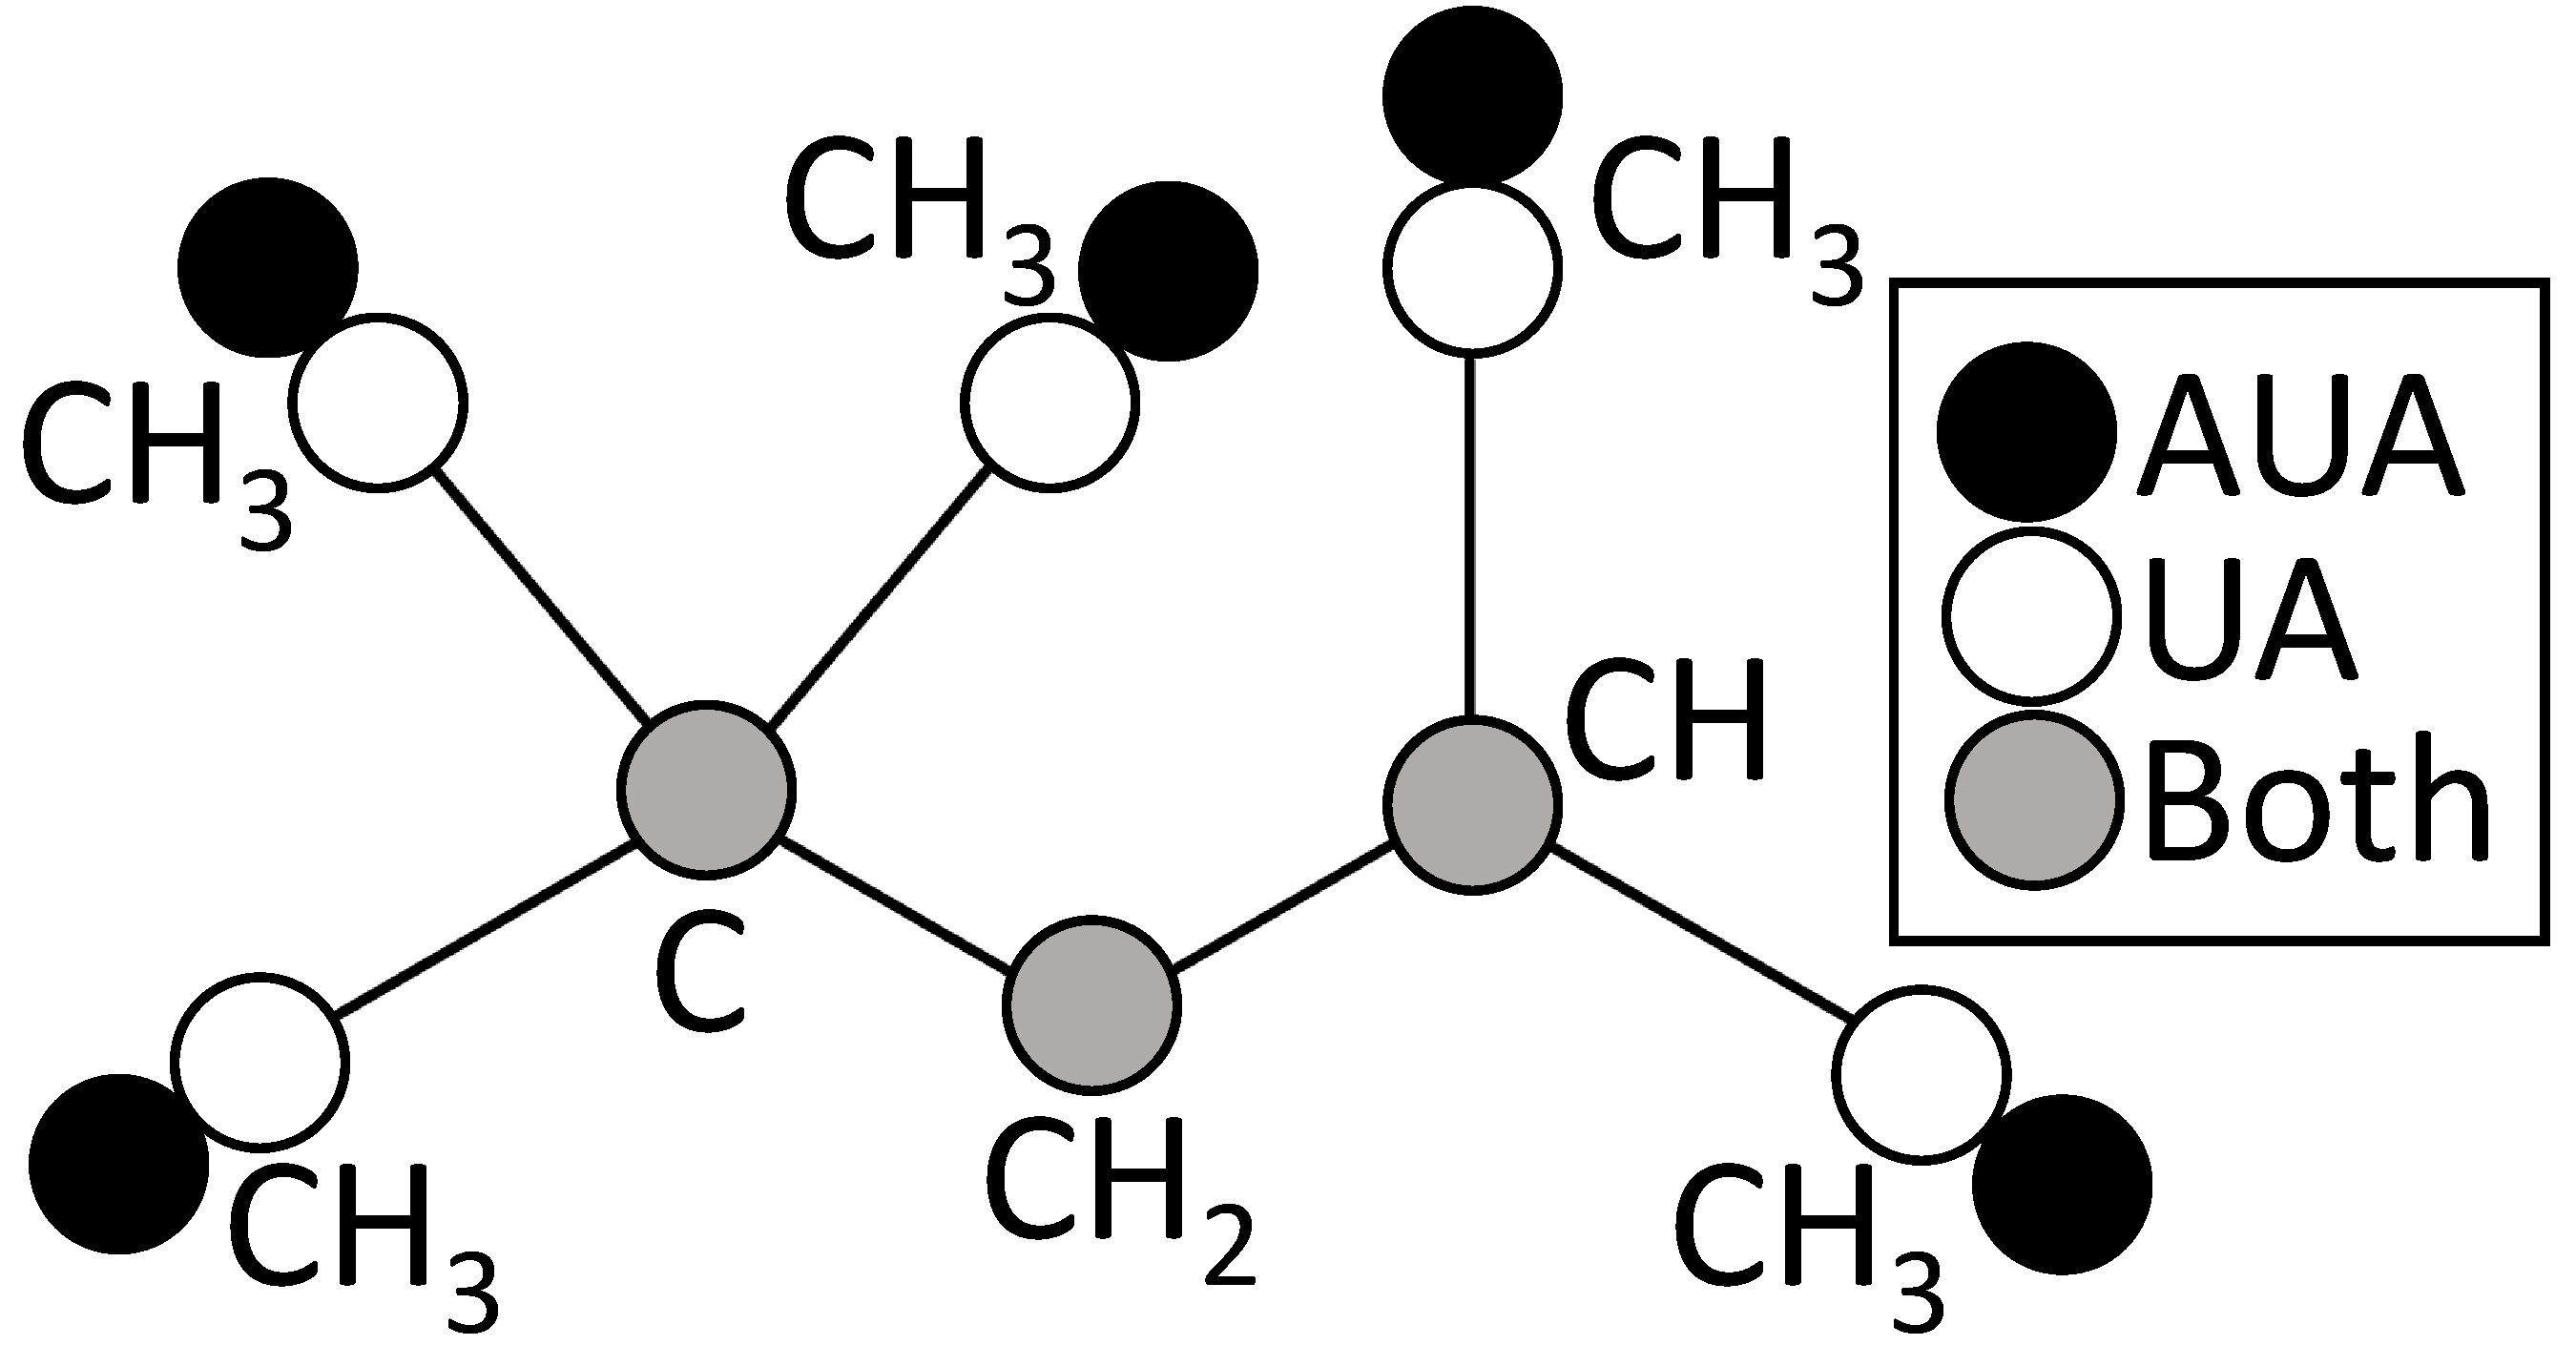
\includegraphics[width=3.2in]{AUA_isooctane}
	\caption{If only the terminal sites have an anisotropic displacement (e.g. TAMie), AUA force fields have the same complexity as UA force fields since the only difference is a longer effective bond-length for the CH$_3$ sites. Note that the AUA4 representation of isooctane requires a more complicated shifting of CH$_2$ and CH sites than that depicted here.}
	\label{fig:AUA_isooctane}
\end{figure}

\begin{table}[h!]
%MRS2: suggest using two different notations for the two situations (not there vs more complicated) rather than just N/A for both.
%RAM2: Yeah, I had that originally but then I tried to get too concise.
	\caption{Effective bond-lengths in units of nm for terminal (CH$_3$) UA or AUA interaction sites. Empty table entries for Exp-6 and TraPPE-2 denote that the force field does not contain the corresponding interaction site type. Empty table entries in AUA4 arise because this force field uses a more complicated construct than the simple effective bond-length approach. Specifically, AUA4 requires CH$_2$ and CH interaction sites that are not along the C-C bond axis.} \label{tab:bond-lengths}
	\begin{center}
		\begin{tabular}{|c|c|c|c|c|c|}
			\hline
			Bond & TraPPE, Potoff & TAMie & Exp-6 & AUA4 & TraPPE-2 \\ \hline
			CH$_3$-CH$_3$ & 0.154 & 0.194 & 0.1839 & 0.1967 & 0.230 \\ 
			CH$_3$-CH$_2$ & 0.154 & 0.174 & 0.1687 & -- & -- \\ 
			CH$_3$-CH & 0.154 & 0.174 & -- & -- & -- \\
			CH$_3$-C & 0.154 & 0.174 & -- & 0.1751 & -- \\
			\hline
		\end{tabular}
	\end{center} 
\end{table}

%%%% Old table
%\begin{table}[h!]
%	\caption{Effective bond-lengths in units of nm for terminal (CH$_3$) UA or AUA interaction sites. ``Not-applicable'' (``N/A'') signifies that the force field either does not include these site types (e.g. Exp-6 and TraPPE-2) or that a more complicated notation than a simple effective bond-length is required to adequately represent the force field (i.e. AUA4).} \label{tab:bond-lengths}
%	\begin{center}
%		\begin{tabular}{|c|c|c|c|c|c|}
%			\hline
%			Bond & TraPPE, Potoff & TAMie & Exp-6 & AUA4 & TraPPE-2 \\ \hline
%			CH$_3$-CH$_3$ & 0.154 & 0.194 & 0.1839 & 0.1967 & 0.230 \\ 
%			CH$_3$-CH$_2$ & 0.154 & 0.174 & 0.1687 & N/A & N/A \\ 
%			CH$_3$-CH & 0.154 & 0.174 & N/A & N/A & N/A \\
%			CH$_3$-C & 0.154 & 0.174 & N/A & 0.1751 & N/A \\
%			\hline
%		\end{tabular}
%	\end{center} 
%\end{table}

The angle and dihedral energies are computed using the same functional forms for each force field. Angular bending interactions are evaluated using a harmonic potential:
\begin{equation}
u^{\rm bend} = \frac{k_\theta}{2} \left(\theta-\theta_0\right)^2
\end{equation}
where $u^{\rm bend}$ is the bending energy, $\theta$ is the instantaneous bond angle, $\theta_0$ is the equilibrium bond angle, and $k_\theta$ is the harmonic force constant which is equal to 62500 K/rad$^2$ for all bonding angles. Dihedral torsional interactions are determined using a cosine series:
\begin{equation}
u^{\rm tors} = c_1 [1+\cos{\phi}] + c_2 [1-\cos{2\phi}] + c_3 [1+\cos{3\phi}]
\end{equation}
where $u^{\rm tors}$ is the torsional energy, $\phi$ is the dihedral angle and $c_i$ are the Fourier constants. The equilibrium bond angles and torsional parameters are found in Tables \ref{tab:angles}-\ref{tab:torsions}, respectively. Note that the Errington $c_i$ values for CH$_x$-CH$_2$-CH$_2$-CH$_y$ are a factor of two less than those reported in Table \ref{tab:torsions}. 
%MRS2: note that there are multiple ways to represent the same torsion
%(1-2-3-4 and 4-3-2-1), and in some case, the barriers are lower for torsional parameters
%because the torsion is applied to both representations.  Is that the case at all in any of these?
%RAM2: We should talk about this. I have copied the torsions exactly as they are presented in the literature for the force field developers.
\begin{table}[h!]
	\caption{Equilibrium bond angles $(\theta_0)$. $x$ and $y$ are values between 0-3.} \label{tab:angles}
	\begin{center}%MRS: would it be more clear with x and y take all values between 0 and 3?
		\begin{tabular}{|c|c|}
			\hline
			Bending sites & $\theta_0$ (degrees) \\ \hline
			CH$_x$-CH$_2$-CH$_y$ & 114.0 \\ 
			CH$_x$-CH-CH$_y$ & 112.0 \\ 
			CH$_x$-C-CH$_y$ & 109.5 \\  
			\hline
		\end{tabular}
	\end{center} 
\end{table}

\begin{table}[h!]
	\caption{Fourier constants $(c_i)$ in units of K. $x$ and $y$ are values between 0-3.} \label{tab:torsions}
	\begin{center}
		\begin{tabular}{|c|c|c|c|c|}
			\hline
			Torsion sites & $c_0$ & $c_1$ & $c_2$ & $c_3$ \\ \hline
			CH$_x$-CH$_2$-CH$_2$-CH$_y$ & 0.0 & 355.03 & -68.19 & 791.32 \\ 
            CH$_x$-CH$_2$-CH-CH$_y$ & -251.06 & 428.73 & -111.85 & 441.27 \\
            CH$_x$-CH$_2$-C-CH$_y$ & 0.0 & 0.0 & 0.0 & 461.29 \\
            CH$_x$-CH-CH-CH$_y$ & -251.06 & 428.73 & -111.85 & 441.27 \\
			\hline
		\end{tabular}
	\end{center} 
\end{table}
%MRS2: suggest putting the equation earlier for reference in the introduction, can rewrite it here if wanted.
%RAM2: We should talk about this
Non-bonded interaction energies and forces between sites located in two different molecules or separated by more than three bonds are calculated using either a Lennard-Jones 12-6, Mie $\lambda$-6, or Buckingham Exponential-6 potential (see Equations \ref{eq:Mie}-\ref{eq:Buckingham}). 
%%%RAM2: Testing out having the equation in the introduction
%The Mie $\lambda$-6 potential is:
%\begin{equation} \label{eq:Mie}
%u^{\rm vdw}(\epsilon,\sigma,\lambda;r) = \left(\frac{\lambda}{\lambda - 6}\right)\left(\frac{\lambda}{6}\right)^{\frac{6}{\lambda - 6}} \epsilon \left[\left(\frac{\sigma}{r}\right)^\lambda - \left(\frac{\sigma}{r}\right)^6\right]
%\end{equation} 
%where $u^{\rm vdw}$ is the van der Waals interaction, $\sigma$ is the distance $(r)$ where $u^{\rm vdw} = 0$, $-\epsilon$ is the energy of the potential at the minimum $\left(\text{i.e. }u^{\rm vdw} = -\epsilon \text{ and } \frac{\partial u^{\rm vdw}}{\partial r} = 0 \text{ for } r=r_{\rm min} \right)$, and $\lambda$ is the repulsive exponent. 
%
%Note that the Mie $\lambda$-6 potential reduces to the LJ 12-6 potential for $\lambda = 12$. Therefore, the LJ 12-6 potential can be considered a special subclass of the Mie $\lambda$-6 potential. It is important to mention that, although an attractive exponent of 6 has a strong theoretical basis, $\lambda = 12$ is a historical artifact that was chosen primarily for computational purposes \cite{Allen1987}. For the same reason (i.e. computational efficiency), a common practice to date is to use integer values of $\lambda$ in Equation \ref{eq:Mie}. The non-bonded force field parameters for TraPPE (and TraPPE-2), Potoff, AUA4, and TAMie are provided in Table \ref{tab:nonbonded params}.
%
%
The non-bonded LJ 12-6 or Mie $\lambda$-6 force field parameters for TraPPE, TraPPE-2, Potoff, AUA4, and TAMie are provided in Table \ref{tab:nonbonded params}. Note that, for computational purposes, a common practice to date is to use integer values of $\lambda$ in Equation \ref{eq:Mie}. 

\begin{table}[h!]
	\caption{Non-bonded (intermolecular) parameters for TraPPE \cite{TraPPE,Martin1999} (and TraPPE-2 \cite{TraPPEUA2}), Potoff \cite{Mie,Potoff_branched}, AUA4 \cite{AUA4,Nieto2008}, and TAMie \cite{TAMie,Weidler2016} force fields. The ``short/long'' Potoff CH and C parameters are included in parenthesis. 
%MRS3: make the lambda entry of the chart wider. 
%RAM3: I had issues with LaTex letting me use specific column widths. I tried using p{2 cm} but I think the multicolumn was a problem.
The ethane specific parameters for TAMie are included in parenthesis.} \label{tab:nonbonded params}
	\begin{center}
		\begin{tabular}{|c|c|c|c|c|c|c|}
			\hline
			\multicolumn{1}{|c}{} & \multicolumn{3}{|c}{TraPPE  (TraPPE-2)} & \multicolumn{3}{|c|}{Potoff (S/L)}  \\ \hline
			United-atom & $\epsilon$ (K) & $\sigma$ (nm) & $\lambda$ & $\epsilon$ (K) & $\sigma$ (nm) & $\lambda$ \\ \hline
			CH$_3$ & 98 (134.5)  & 0.375 (0.352) & 12 & 121.25 & 0.3783 & 16  \\ 
			CH$_2$ & 46 & 0.395 & 12 & 61 & 0.399 & 16 \\ 
			CH & 10 & 0.468 & 12 & 15 (15/14) & 0.46 (0.47/0.47) & 16\\
			C & 0.5 & 0.640 & 12 & 1.2 (1.45/1.2) & 0.61 (0.61/0.62) & 16\\
			\hline
			\multicolumn{1}{|c}{} & \multicolumn{3}{|c}{AUA4} & \multicolumn{3}{|c|}{TAMie} \\ \hline
			CH$_3$ & 120.15  & 0.3607 & 12 & 136.318 (130.780) & 0.36034 (0.36463) & 14 \\ 
			CH$_2$ & 86.29 & 0.3461 & 12 & 52.9133 & 0.40400 & 14 \\ 
			CH & 50.98 & 0.3363 & 12 & 14.5392 & 0.43656 & 14\\
			C & 15.04 & 0.244 & 12 & -- & -- & --\\
			\hline
		\end{tabular}
	\end{center} 
\end{table}

%\begin{table}[h!]
%	\caption{Non-bonded (intermolecular) parameters for TraPPE-UA, Potoff, and TAMie force fields. The ``short/long'' Potoff CH and C parameters are included in parenthesis. The ethane specific parameters for TAMie are included in parenthesis.} \label{tab:nonbonded params}
%	\begin{center}
%		\begin{tabular}{|c|c|c|c|c|c|c|c|c|c|}
%			\hline
%			\multicolumn{1}{|c}{} & \multicolumn{3}{|c}{TraPPE-UA} & \multicolumn{3}{|c}{Potoff} & \multicolumn{3}{|c|}{TAMie} \\ \hline
%			United-atom & $\epsilon$ (K) & $\sigma$ (nm) & $\lambda$ & $\epsilon$ (K) & $\sigma$ (nm) & $\lambda$ & $\epsilon$ (K) & $\sigma$ (nm) & $\lambda$ \\ \hline
%			CH$_3$ & 98 & 0.375 & 12 & 121.25 & 0.3783 & 16 & 136.318 (130.780) & 0.36034 (0.36463) & 14 \\ 
%			CH$_2$ & 46 & 0.395 & 12 & 61 & 0.399 & 16 & 52.9133 & 0.40400 & 14\\ 
%			CH & 10 & 0.468 & 12 & 15 (15/14) & 0.46 (0.47/0.47) & 16 & 14.5392 & 0.43656 & 14 \\
%			C & 0.5 & 0.640 & 12 & 1.2 (1.45/1.2) & 0.61 (0.61/0.62) & 16 & N/A & N/A & N/A \\
%			\hline
%		\end{tabular}
%	\end{center} 
%\end{table}
%
%\begin{table}[h!]
%	\caption{Non-bonded (intermolecular) parameters for TraPPE, Potoff, and TAMie force fields. The TraPPE-2 parameters for CH$_3$ are included in parenthesis. The ``short/long'' Potoff CH and C parameters are included in parenthesis. The ethane specific parameters for TAMie are included in parenthesis.} \label{tab:nonbonded params}
%	\begin{center}
%		\begin{tabular}{|c|c|c|c|c|c|c|c|c|c|}
%			\hline
%			\multicolumn{1}{|c}{} & \multicolumn{2}{|c}{TraPPE LJ 12-6} & \multicolumn{2}{|c}{Potoff Mie 16-6} & \multicolumn{2}{|c|}{TAMie Mie 14-6} \\ \hline
%			United-atom & $\epsilon$ (K) & $\sigma$ (nm) & $\epsilon$ (K) & $\sigma$ (nm) & $\epsilon$ (K) & $\sigma$ (nm) \\ \hline
%			CH$_3$ & 98 (134.5)  & 0.375 (0.352) & 121.25 & 0.3783 & 136.318 (130.780) & 0.36034 (0.36463) \\ 
%			CH$_2$ & 46 & 0.395 & 61 & 0.399 & 52.9133 & 0.40400 \\ 
%			CH & 10 & 0.468 & 15 (15/14) & 0.46 (0.47/0.47)  & 14.5392 & 0.43656  \\
%			C & 0.5 & 0.640 & 1.2 (1.45/1.2) & 0.61 (0.61/0.62)& N/A & N/A  \\
%			\hline
%		\end{tabular}
%	\end{center} 
%\end{table}
%
%\begin{table}[h!]
%	\caption{Non-bonded (intermolecular) parameters for TraPPE-2 and AUA4. Only the , Potoff, and TAMie force fields. The ``short/long'' Potoff CH and C parameters are included in parenthesis.} \label{tab:nonbonded params2}
%	\begin{center}
%		\begin{tabular}{|c|c|c|c|c|c|c|}
%			\hline
%			\multicolumn{1}{|c}{} & \multicolumn{3}{|c}{TraPPE-UA} & \multicolumn{3}{|c|}{Potoff} \\ \hline
%			United-atom & $\epsilon$ (K) & $\sigma$ (nm) & $\lambda$ & $\epsilon$ (K) & $\sigma$ (nm) & $\lambda$ \\ \hline
%			CH$_3$ & 98 & 0.375 & 12 & 121.25 & 0.3783 & 16  \\ 
%			CH$_2$ & 46 & 0.395 & 12 & 61 & 0.399 & 16 \\ 
%			CH & 10 & 0.468 & 12 & 15 (15/14) & 0.46 (0.47/0.47) & 16 \\
%			C & 0.5 & 0.640 & 12 & 1.2 (1.45/1.2) & 0.61 (0.61/0.62) & 16 \\
%			\hline
%		\end{tabular}
%	\end{center} 
%\end{table}

%%%RAM2: Moved to introduction
%The Errington force field utilizes a Buckingham exponential-6 (Exp-6) model:
%\begin{equation} \label{eq:Buckingham}
%u^{\rm vdw}(\epsilon,r_{\rm min},\alpha;r) = 
%\begin{cases}
%\frac{\epsilon}{1-\frac{6}{\alpha}} \left[\frac{6}{\alpha} \exp\left(\alpha\left[1-\frac{r}{r_{\rm min}}\right]\right) - \left(\frac{r_{\rm min}}{r}\right)^6\right] & \text{for}\ r>r_{\rm max} \\
%\infty           & \text{for}\ r<r_{\rm max}
%\end{cases}
%\end{equation}
%where $u^{\rm vdw}$, $\epsilon$, and $r$ are the same as in Equation \ref{eq:Mie}, $r_{\rm min}$ is the distance that corresponds to the minimum in the potential (i.e $u^{\rm vdw}(r_{\rm min})=-\epsilon$), $\alpha$ is a Buckingham exponential-6 parameter, and $r_{\rm max}$ is the smallest positive value for which $\frac{du^{\rm vdw}}{dr}=0$. The Errington non-bonded parameters are found in Table \ref{tab:nonbonded Exp6}. (Note that Errington reported values for $\epsilon$, $\sigma$, and $\alpha$. We computed $r_{\rm min}$ and $r_{\rm max}$ to facilitate compatibility with Equation \ref{eq:Buckingham} and future validation of our results.)
%
%\begin{table}[h!]
%	\caption{Non-bonded (intermolecular) parameters for Errington Exp-6 force field.} \label{tab:nonbonded Exp6}
%	\begin{center}
%		\begin{tabular}{|c|c|c|c|c|c|}
%			\hline
%			United-atom & $\epsilon$ (K) & $\sigma$ (nm) & $\alpha$ & $r_{\rm min}$ (nm) & $r_{\rm max}$ (nm)  \\ \hline
%			CH$_3$ & 129.6  & 0.3679 & 16 & 0.4094 & 0.0574 \\ 
%			CH$_2$ & 73.5 & 0.400 & 22 & 0.436 & 0.0221 \\ \hline
%		\end{tabular}
%	\end{center} 
%\end{table}

%The Errington force field utilizes a Buckingham exponential-6 (Exp-6) model. 

The Errington Exp-6 non-bonded parameters are found in Table \ref{tab:nonbonded Exp6}. Note that Errington reported values for $\epsilon$, $\sigma$, and $\alpha$. We computed $r_{\rm min}$ and $r_{\rm max}$ to facilitate compatibility with Equation \ref{eq:Buckingham} and future validation of our results.

\begin{table}[h!]
	\caption{Non-bonded (intermolecular) parameters for Errington Exp-6 force field.} \label{tab:nonbonded Exp6}
	\begin{center}
		\begin{tabular}{|c|c|c|c|c|c|}
			\hline
			United-atom & $\epsilon$ (K) & $\sigma$ (nm) & $\alpha$ & $r_{\rm min}$ (nm) & $r_{\rm max}$ (nm)  \\ \hline
			CH$_3$ & 129.6  & 0.3679 & 16 & 0.4094 & 0.0574 \\ 
			CH$_2$ & 73.5 & 0.400 & 22 & 0.436 & 0.0221 \\ \hline
		\end{tabular}
	\end{center} 
\end{table}

Non-bonded interactions between two different site types (i.e. cross-interactions) are determined using Lorentz-Berthelot combining rules \cite{Allen1987} for $\epsilon$ and $\sigma$, an arithmetic mean for the repulsive exponent $\lambda$ (as recommended in Reference \citenum{Mie}), and a geometric mean for $\alpha$ (as recommended in Reference \citenum{Exp6}):
\begin{equation} \label{eq:Lorentz-Berthelot_eps}
\epsilon_{ij} = \sqrt{\epsilon_{ii} \epsilon_{jj}}
\end{equation}
\begin{equation} \label{eq:Lorentz-Berthelot_sig}
\sigma_{ij} = \frac{\sigma_{ii} + \sigma_{jj}}{2}
\end{equation}
\begin{equation} \label{eq:Lorentz-Berthelot_lam}
\lambda_{ij} = \frac{\lambda_{ii} + \lambda_{jj}}{2}
\end{equation}
\begin{equation} \label{eq:Lorentz-Berthelot_alpha}
\alpha_{ij} = \sqrt{\alpha_{ii} \alpha_{jj}}
\end{equation}
where the $ij$ subscript refers to cross-interactions and the subscripts $ii$ and $jj$ refer to same-site interactions. 

%\begin{enumerate}
%	\item For each compound studied, we use a united-atom representation as defined by the TraPPE (and Mie) force fields. For normal and branched alkanes this consists of CH3, CH2, CH, and C sites.
%	\item We use fixed bond-lengths, harmonic angles, cosine series for torsions, and exclude 1-4 nonbonded interactions 
%	\item Bonded parameters are provided in supporting information
%	\item Nonbonded interactions for intermolecular and intramolecular sites separated by more than 3 bonds are represented using a Mie potential, which can be viewed as a generalized Lennard-Jones
%%MRS: need to make it clearer what your hypothesis is, then.  If it's just ``Mie not good'', then restrict it.  If the goal is to find something better, which might be more impactful. But it can be a short paper. If its ``nothing existing is good'', then will need to include others.
%%MRS: Looking more carefully, I think your main idea is not that Mie isn't that good, but NONE of the existing UA isotropic functional forms are not that good. That is a more general conclusion, but doesn't force you to posit a new one within the scope of this paper. It does make a stronger statement; if you say ``Mie isn't good'', then people will wonder, why don't you just say what is good.  If you say none of the ``standard UA approaches are good'' that's more important.   You MIGHT need to say ``But this approach can work''.  That might require more work than there is time for this time.
%	\item (Maybe include Exp-6 and extended Lennard-Jones, i.e. 12-10-8-6)
%%MRS: when you say ``rigorous bayesian'', you should be more specific what analysis doing.
%%MRS: My instinct, if ``anisotropic'' UA works for this system, it might not be worth it that much to develop a new functional form.  Unless there's strong reason it might be useful more generally.  we can discuss goals a bit; it really depends on goals. 
%\end{enumerate}

\section{Case study} \label{Case Study}

The purpose of this case study is to demonstrate that the existing UA and AUA force fields for normal and branched alkanes that were parameterized with VLE properties do not predict the proper $P \rho T$ behavior at higher temperatures and pressures (with the exception of ethane for the TraPPE-2 potential). Figures \ref{fig:IC_normal_alkanes}--\ref{fig:IC_branched_alkanes} plot the compressibility factor with respect to inverse temperature for \textit{n}-alkanes and branched alkanes, respectively. Note that saturation corresponds to $Z \approx 0$ for each isochore. The ``Potoff'' results in Figure \ref{fig:IC_branched_alkanes} are only for the the ``short/long'' model, since the ``short/long'' model is more accurate than the ``generalized'' model (available in Section \ref{Potoff Generalized} of Supporting Information). 

%The results for the ``generalized'' model do not provide any additional insight but are found in Section \ref{Potoff Generalized} of Supporting Information.

%The ``Potoff'' results in Figure \ref{fig:IC_branched_alkanes} are only for the the ``short/long'' model, since the ``short/long'' model is more accurate than the ``generalized'' model. Specifically, isobutane and neopentane use the ``short'' parameters, while isohexane and isooctane use the ``long'' parameters. The results for the ``generalized'' model do not provide any additional insight but are found in the Supporting Information. 

%Several force fields in the literature have been optimized to agree with VLE properties for normal and branched alkanes. Two of the most widely used united-atom based force fields are the TraPPE LJ 12-6 and Potoff Mie 16-6.

%It has been demonstrated that the united-atom LJ 12-6 potential cannot adequately estimate both $\rho_{\rm l}^{\rm sat}$ and $P_{\rm v}^{\rm sat}$. By contrast, when properly optimized, the Mie 16-6 potential can accurately predict both $\rho_{\rm l}^{\rm sat}$ and $P_{\rm v}^{\rm sat}$ over a wide temperature range. However, there is some concern that increasing the repulsive exponent (in this case, from 12 to 16) might have some undesirable consequences, especially at high pressures, where close range interactions will become more significant.

%\afterpage{%
\begin{figure}[p!]
	\centering
	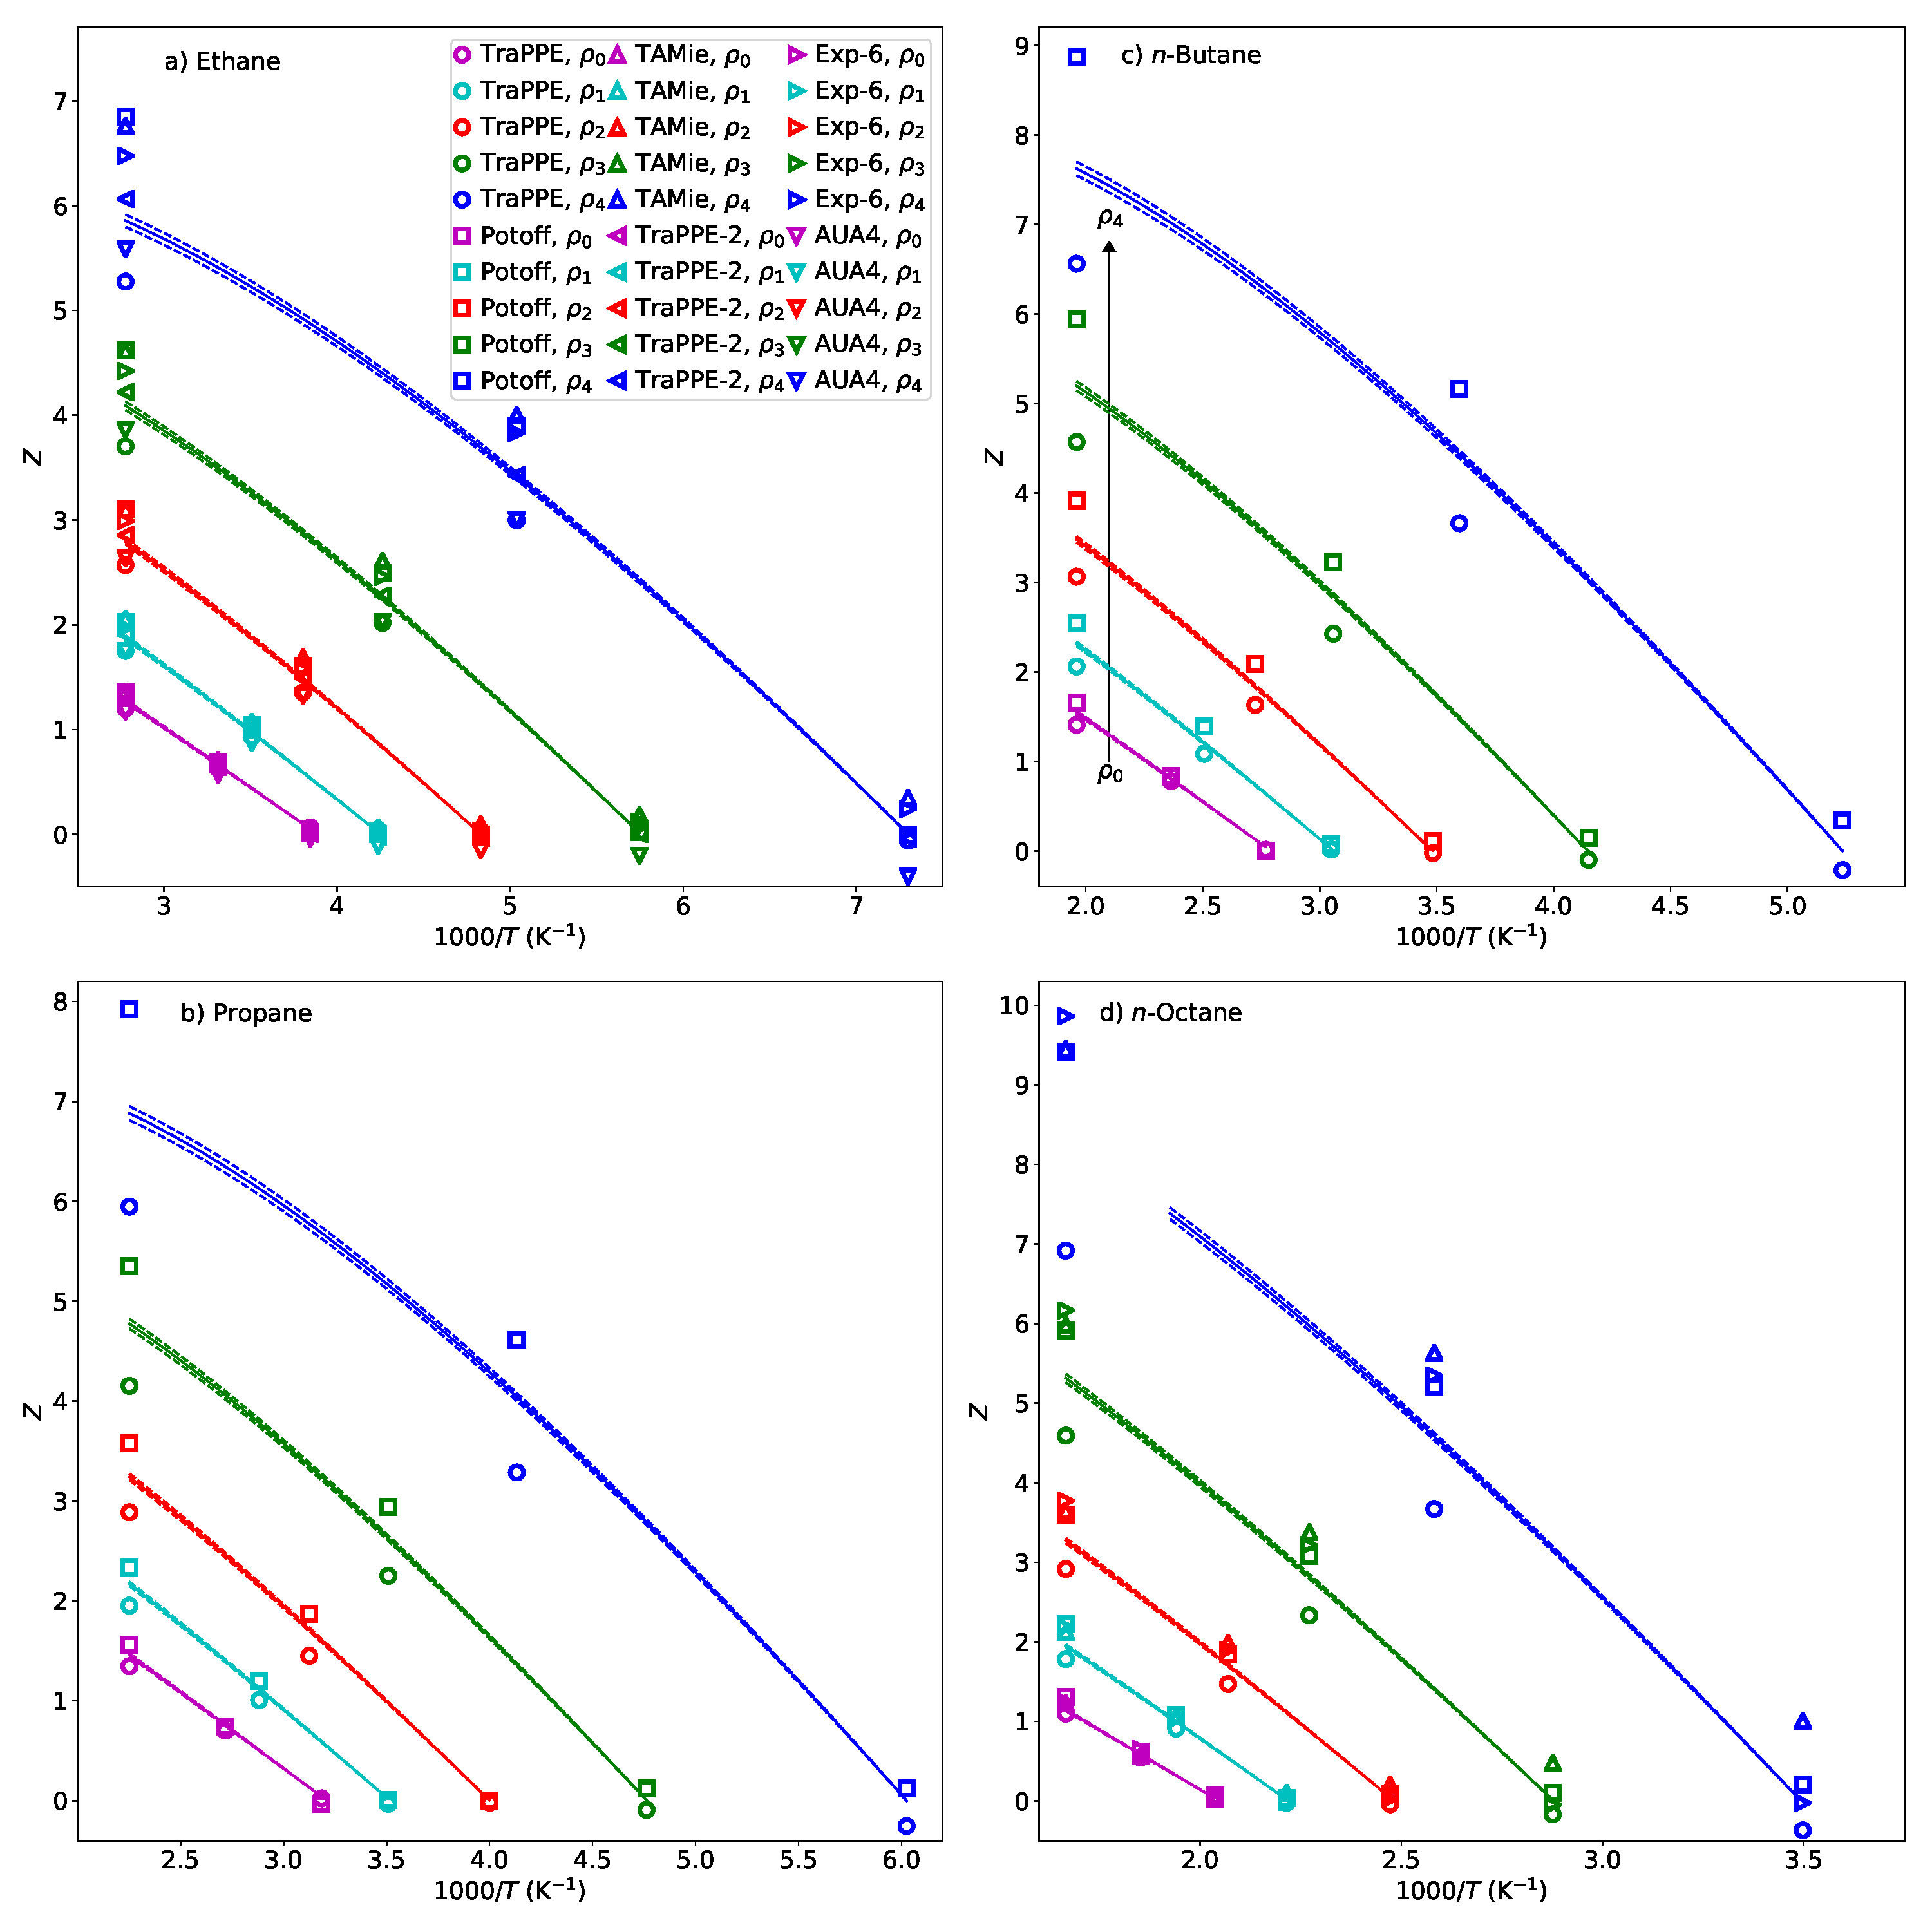
\includegraphics[width=6.4in]{IC_normal_alkanes_all_models}
%MRS3: probably should explicitly give the colors along with the rhos.
	\caption{Compressibility factors $(Z)$ along isochores agree at saturation $(Z \approx 0)$ but deviate strongly at higher pressures. Densities are distinguished by color, increase vertically, and are labeled such that $\rho_0 < \rho_1 < \rho_2 < \rho_3 < \rho_4$.  Panels a)-d) correspond to ethane, propane, \textit{n}-butane, and \textit{n}-octane, respectively.
% This was outdated information. I have removed the error bars for clarity.
% TraPPE and Potoff simulation results are depicted using open circles and squares, respectively, with error bars representing two times the standard deviation of the fluctuations from a single simulation. 
%MRS2: could also add it's approximately a 95% confidence interval.  Also, when you say standard deviation of the fluctuations from a single simulation, do you mean the standard error in the mean? Standard deviation in fluctuations from a simulation are larger than the estimated error in the mean by a factor of (Nsamples-1)^-1/2.
%RAM2: Yes, my error bars over-estimated the uncertainty, and they were still only one symbol size. So I decided to be less explicit since the error bars are really quite small. 
Solid lines represent REFPROP correlations, with dashed lines representing a 1\% uncertainty in REFPROP values. Simulation error bars are approximately one symbol size.}
	\label{fig:IC_normal_alkanes}
\end{figure}
%}

%\newpage

\begin{figure}[p!]
%MRS2: suggest making 2 and 3 one page-sized figure? Could make symbol lines a one notch thicker.  If 2 pages, I would repeat the legend.
%RAM2: My intention was for these to be page-sized figures. 
%RAM2: Made symbol edges thicker. 
%RAM2: Repeated the legend
	\centering
	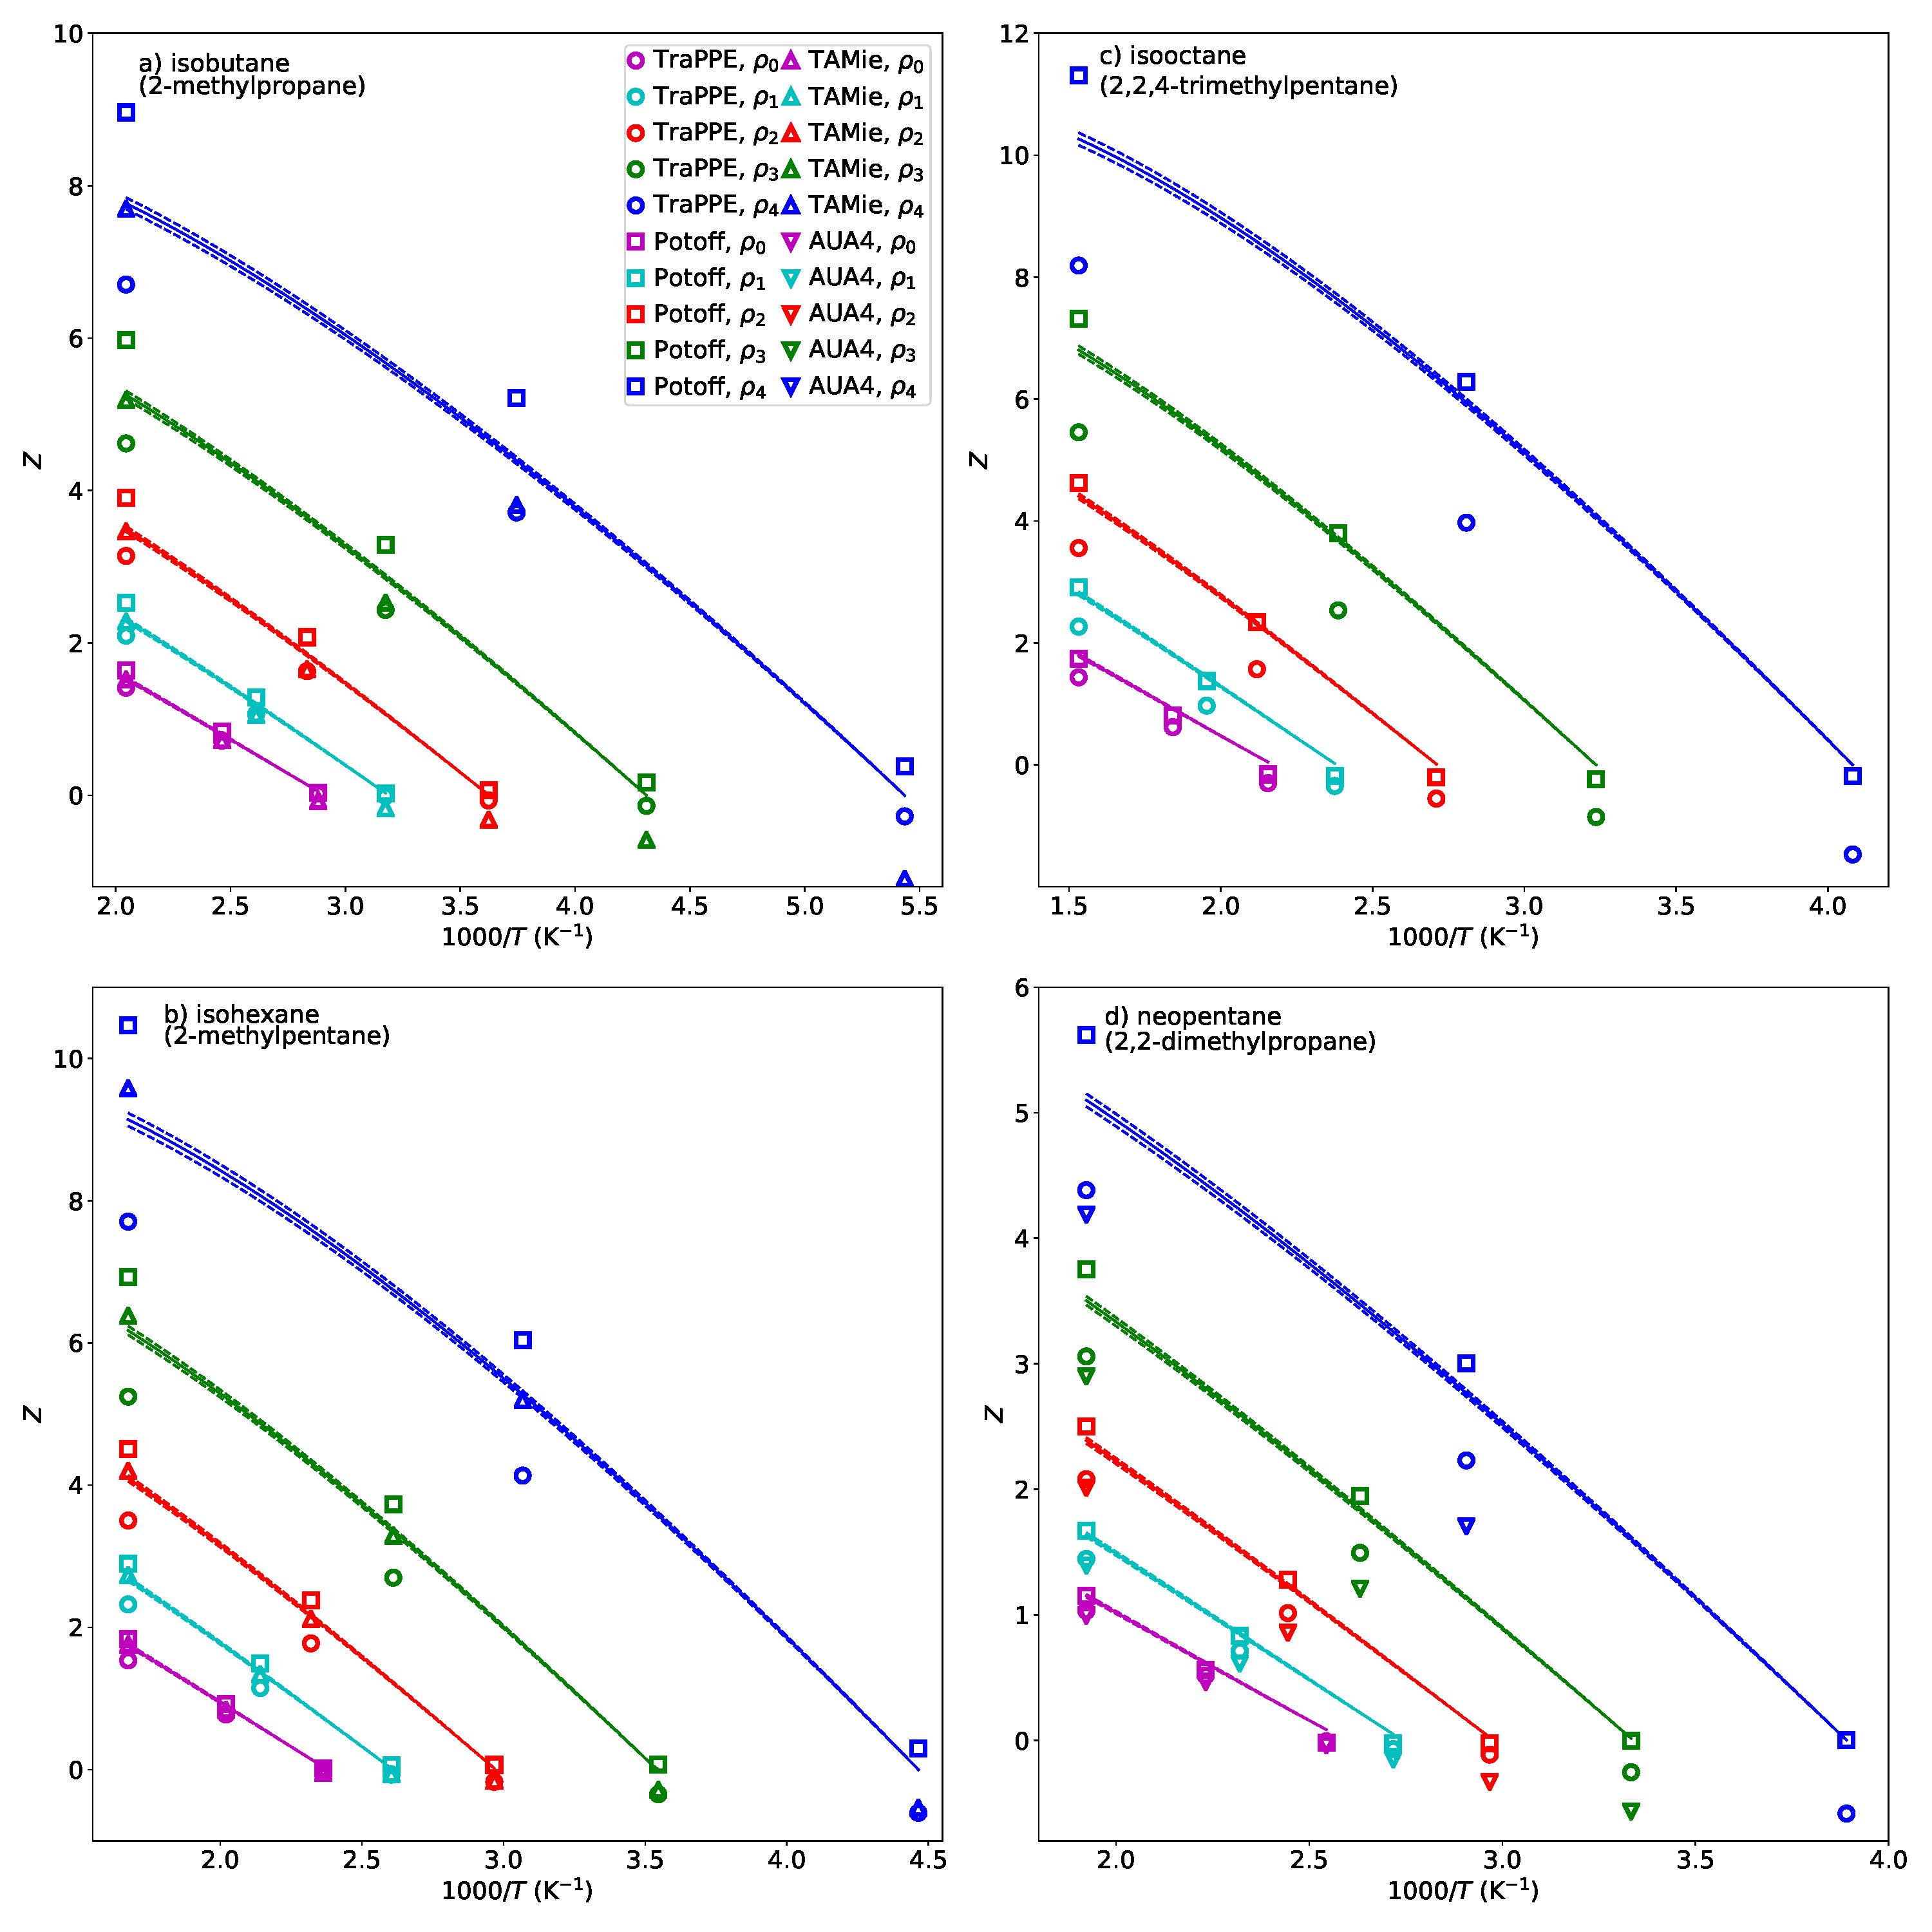
\includegraphics[width=6.4in]{IC_branched_alkanes_all_models}
	\caption{Compressibility factors $(Z)$ along isochores for branched alkanes are not as accurate as normal alkanes at saturation $(Z \approx 0)$ and deviate strongly at higher pressures. Panels a)-d) correspond to isobutane, isohexane, isooctane, and neopentane, respectively. Symbols, lines, uncertainties, and formatting are the same as those in Figure \ref{fig:IC_normal_alkanes}. The Potoff results for isobutane and neopentane use the ``short'' parameters, while isohexane and isooctane use the ``long'' parameters (see Table \ref{tab:nonbonded params}).}
	\label{fig:IC_branched_alkanes}
\end{figure}

%\newpage

% I am going to change isopentane to isohexane so that it uses Potoff 'long', to have a better representation of compounds.


Figure \ref{fig:IC_normal_alkanes} demonstrates that the existing literature force fields for \textit{n}-alkanes, while accurate for VLE $(Z \approx 0)$, do not capture the correct $P \rho T$ behavior at high pressures $(P^{\rm high})$, i.e. $Z$ at the higher temperatures $(T > T^{\rm sat})$ and highest isochore densities $(\rho_3$ and $\rho_4)$. 
%MRS3: I wonder ``if correct $P \rho T$ behavior at high pressures $(P^{\rm high})$'', should be made more specific. 
%RAM3: Made it a little more specific
Figure \ref{fig:IC_branched_alkanes} shows the same erroneous trend in $Z$ for branched alkanes. Note that the error in $Z$ at high temperatures is less obvious because these force fields are typically not as reliable at predicting VLE for branched alkanes as for \textit{n}-alkanes, i.e. notice the large deviations at $Z \approx 0$. That being said, it is clear in both Figures \ref{fig:IC_normal_alkanes}-\ref{fig:IC_branched_alkanes} that none of the force fields adequately reproduces $Z$ over the entire temperature range, or the slope of $Z$ with respect to inverse $T$.

% Note that the error in the slope of $Z$ with respect to inverse $T$ is less obvious because these force fields are typically less reliable at VLE for branched alkanes than for \textit{n}-alkanes, i.e. notice the large deviations at $Z \approx 0$.

%Figure \ref{fig:IC_branched_alkanes} shows that these force fields are typically less reliable at VLE for branched alkanes than for \textit{n}-alkanes, i.e. notice the large deviations at $Z \approx 0$. More importantly, the same erroneous trend in $Z$ is observed as in Figure \ref{fig:IC_normal_alkanes}. 

%Figure \ref{fig:IC_branched_alkanes} shows that these force fields are typically less reliable at VLE for branched alkanes than for \textit{n}-alkanes, i.e. notice the large deviations at $Z \approx 0$. More importantly, the same erroneous trend in $Z$ is observed as in Figure \ref{fig:IC_normal_alkanes}. 

A surprising trend is that the Errington (AUA Exp-6) model has a positive bias at high pressures. This appears to suggest that the repulsive barrier is too steep, despite the fact that the Exp-6 model is typically considered softer than the LJ 12-6. However, for $\alpha_{\rm CH_3} = 16$, the Exp-6 is less repulsive than the LJ 12-6 only at very short distances, i.e. $r < 0.7 r_{\rm min}$, while it is actually somewhat more repulsive for the closest-range distances sampled in molecular dynamics at these conditions, i.e. $0.7 r_{\rm min} < r < r_{\rm min}$.  
%%RAM2: I decided to remove some of this since it is not very useful or convincing. Exp-6 decays faster than r^-12, is softer than r^-12 at very short distances, but in the range 0.7rmin-rmin it is actually a bit harder
%Therefore, it is more likely that the Exp-6 repulsive forces are over-predicted only for the close-range distances that are sampled in molecular dynamics, i.e. $0.8 \sigma < r < r_{\rm min}$. Alternatively, since the exponential contribution is non-negligible for $r_{\rm min} < r < 1.5 \sigma$, it is possible that the tail does not decay to zero quickly enough and, therefore, the Exp-6 under-predicts the attractive forces in this region. 
%
More definitive and straight-forward conclusions regarding the shape of the Mie $\lambda$-6 repulsive barrier are possible by directly comparing different values of $\lambda$. 
 
In general, 
%MRS: clarified, bias singular suggests it's the same, but each is different.
%a clear bias is
clear systematic biases are observed for the LJ 12-6 potentials (TraPPE-UA and AUA4) and the Mie $\lambda$-6 potentials (Potoff and TAMie). Specifically, 
%MRS4: techniclly, LJ 12-6 is a mie lambda-6 potential - be a bit clearer?
the LJ 12-6 and Mie $\lambda$-6 potentials under- and over-predict $Z$ at high pressures, respectively. These results are intuitive as the repulsive barriers are steeper for the respective Mie 16-6 and 14-6 potentials of the Potoff and TAMie force fields. 
% as the impact of $\lambda$ is more directly comparable.

% or that the attractive forces are under-predicted for $r > r_{\rm min}$.  

%This suggests that an exponential repulsive barrier is too steep, at least for the distances that are sampled at these state points.
%MRS2: could suggest that the size parmeter is not chosen well; far enough up, it could be sufficiently soft, but if the size parameter isn't quite right, it could be too stiff in this region.
%RAM2: True. Really it just shows that the repulsive forces are either too high or that the attractive forces are too weak. So it can be that the well has too steep of a slope or that the tail is too gradual.

%MRS2: I don't know that TraPPE-2 ``reproduces'', since at the highest P, it is outside the REFPROP bounds. And somewhat off at high T.  Maybe stating that it's the best of them.  Can you make a more quantitiatve statement, perhaps a RMS error compared to the other models, rather than making a binary statement (unless there are clear criteria for the binary statement, of course - which would involve a definition of ``reproduces'').
%RAM2: True. The TraPPE-2 is not perfect. It is still outside of the REFPROP uncertainty. I have tried rewording this.
%MRS2: maybe reverse the density ordering labeling? Intiuitively, one would expect rho_i+1 > rho_i.
%RAM2: Done
The one exception to this trend is the TraPPE-2 model for ethane, which has the most accurate prediction of the entire $P \rho T$ phase space simulated. Specifically, TraPPE-2 reproduces $Z$ to within the REFPROP uncertainties for all state points except at $P^{\rm high}$, where the average percent deviation (AD\%) relative to the REFPROP correlations is still only 3\%.

%the two highest densities along the supercritical isotherm, i.e. $T=T^{IT}$ and $\rho = \rho_3$ or $\rho_4$. The average percent deviation (AD\%) relative to the REFPROP correlations is only 3\% for pressure at these state points $(P^{\rm high})$. 

The performance of TraPPE-2 is somewhat surprising considering this force field has only three fitting parameters ($\epsilon$, $\sigma$, and the effective bond-length) while the TAMie model has these three parameters and an additional fitting parameter $(\lambda)$. It is possible that a four parameter optimization, such as that used by TAMie, is overfit to the VLE data and would perform better if high pressure $P \rho T$ data were included in the parameterization. Furthermore, it is important to note that TraPPE-2 uses a much longer effective bond-length of 0.230 nm while TAMie did not consider bond-lengths larger than 0.194 nm. Therefore, the fact that the TraPPE-2 force field extrapolates to high pressures better than TAMie suggests that, at high pressures, it is important to account for hydrogens with a longer effective bond-length than that typically used for AUA models (see Table \ref{tab:bond-lengths}). It seems logical that at even higher pressures an AA model may become necessary.

%. either explicitly (AA model) or  It is also possible that a four parameter optimization, such as that used by TAMie, is overfit to the VLE data and would perform better if high pressure $P \rho T$ data were included in the parameterization.

Unfortunately, a direct comparison of the non-bonded interactions for AUA force fields is difficult because each model has a different anisotropic displacement, i.e. effective bond-length. 
%MRS2: do you need both i.e. and parentheses above?
%RAM2: No. That is just my tendency.
By contrast, 
%MRS2: nominalization.
%a comparison of 
comparing TraPPE-UA and Potoff is straightforward because they use the same bond-lengths and the same non-bonded Mie $\lambda$-6 potential (Equation \ref{eq:Mie}). For example, since the TraPPE-UA (LJ 12-6) potential under-predicts $Z$ and the Potoff (UA Mie 16-6) potential over-predicts $Z$, it seems reasonable that a UA Mie 13-6, 14-6, or 15-6 model 
%MRS2: suggest
%would 
could
demonstrate the proper trend (although it is important to remember that certain values of $\lambda$ cannot reproduce both $\rho_{\rm l}^{\rm sat}$ and $P_{\rm v}^{\rm sat}$).

To investigate this hypothesis, the remainder of this document focuses on the UA Mie $\lambda$-6 potential, where all bond-lengths are 0.154 nm to be consistent with the TraPPE and Potoff UA models.
%MRS3: hmmm.  May need to justify this value; maybe one of them would work with 0.160, for example.  That hasn't been ruled out. 
%RAM3: Well we are defining UA as having a 0.154 nm bond-length for terminal sites, a longer bond-length for terminal sites is an AUA model. It is true that a different bond-length for non-terminal (CH2) bonds could show a different result. However, we need to keep this fixed for a rigorous comparison with TraPPE and Potoff. I have mentioned that now.
Specifically, we perform a Bayesian uncertainty quantification analysis to determine if there exists a set of $\epsilon$, $\sigma$, and $\lambda$ that reasonably predicts $\rho_{\rm l}^{\rm sat}$, $P_{\rm v}^{\rm sat}$, and $P^{\rm high}$. The results in Section \ref{Results} demonstrate that the optimal value of $\lambda$ for predicting $P \rho T$ of supercritical fluids and compressed liquids is not capable of predicting VLE properties accurately, and vice-versa. 

%To understand this point, it is important to remember that the TraPPE-UA LJ 12-6 force field was optimized using only $\rho_{\rm l}^{\rm sat}$ because the UA LJ 12-6 model cannot adequately predict both $\rho_{\rm l}^{\rm sat}$ and $P_{\rm v}^{\rm sat}$.

%However, as demonstrated in Section \ref{Results}, there does not exist a set of $\epsilon$, $\sigma$, and $\lambda$ that reasonably predicts $\rho_{\rm l}^{\rm sat}$, $P_{\rm v}^{\rm sat}$, and $P \rho T$ of supercritical fluids and compressed liquids for the UA model. To understand this point, it is important to remember that the UA LJ 12-6 (TraPPE-UA) force field cannot adequately predict both $\rho_{\rm l}^{\rm sat}$ and $P_{\rm v}^{\rm sat}$. In other words, determining the optimal value of $\lambda$ for predicting $P \rho T$ of supercritical fluids and compressed liquids does not guarantee accurate prediction of $P_{\rm v}^{\rm sat}$. See Section \ref{Results} for a further discussion.



%Although the TAMie potential uses a softer repulsive exponent than Potoff (14 instead of 16), it consistently over-predicts the pressure for supercritical fluids and compressed liquids. The same is true for the Errington Exp-6 model. By contrast, the TraPPE-2 potential provides extremely reliable estimates of $\rho_{\rm l}^{\rm sat}$, $P_{\rm v}^{\rm sat}$, and the P$\rho$T behavior at high pressures and temperatures. Although the TraPPE-2 model is only available for ethane and ethylene, these results suggest that at extreme pressures either an AUA or AA model should be used to better account for the hydrogens. That being said, alternative functional forms, such as the extended Lennard-Jones, should also be considered.

% although the 12-6 potential is too soft and the 16-6 potential is too hard, the optimal exponent i

%\begin{enumerate}
%	\item Several force fields in the literature have been optimized to agree with VLE properties (TraPPE, Potoff, TraPPE-2, TAMie, Errington, AUA4)
%	\item TraPPE, Potoff, and AUA4 have parameters for each compound studied, while TraPPE-2 only has parameters for ethane, TAMie has parameters for all except isooctane and neopentane (containing a C group), and ErrExp-6 only has parameters for the \textit{n}-alkanes
%%MRS: for figures: be more explicit about what point the data in the figures are supposed to support.
%	\item Figure: Z vs 1000/T for ethane, propane, n-butane, and n-octane
%	\item Figure: Z vs 1000/T for isobutane, isopropane, isohexane, isooctane and neopentane 
%	\item P$\rho$T (Z) trends are inaccurate for both TraPPE and Potoff at high pressures, i.e. non-VLE conditions. Specifically, the TraPPE 12-6 under-predicts while 16-6 over-predicts
%	\item Although these results might suggest that a 14-6 potential would work best, recall that the TraPPE 12-6 does not accurately predict Pvsat. 
%	\item Since TraPPE and Potoff use slightly different objective functions we want to perform an equivalent analysis for different values of lambda
%	\item Hypothesis that we want to test is that there does not exist a set of epsilon, sigma, and lambda that provides reasonable VLE, supercritical fluid, and compressed liquid (for ethane I already know this is not feasible. For n-alkanes I know that the 16-6 cannot accomplish this, but I am not sure about 14-6 or 15-6.)
%	%%% RAM: Do we want to include results for the AUA models in the case study, future work, or supporting information?
%        %%% MRS: it changes the scope a lot.  You have to decide.  ``Not mie'' is simpler, can get out faster.  
%	\item AUA LJ 12-6 is much more accurate for ethane
%	\item AUA Mie 14-6 potential is not much better than UA Mie 16-6 for n-alkanes
%	\item AUA Exp-6 force field is not much better than UA Mie 16-6 for n-alkanes
%	\item No results for AUA4
%\end{enumerate}

%MRS3: methods II is a bad section name; not a typical way of dividing things. . . 
%RAM3: Any suggestions?
\section{Methods II} \label{Methods II}

The results presented in Section \ref{Case Study} demonstrate that none of the literature UA or AUA force fields, parameterized with VLE data, can reproduce the $P \rho T$ behavior for supercritical fluids and compressed liquids. However, there is uncertainty in the non-bonded parameters inherited from the VLE data. Therefore, by considering the inherent uncertainty, it is possible that 
%MRS2: what do you mean by ``equally probably'' here?
%equally probable 
%RAM2: Hopefully it is more clear now
a feasible parameter set exists that adequately predicts VLE and $P^{\rm high}$. By contrast, if none of the $\epsilon$, $\sigma$, and $\lambda$ sets is capable of simultaneously predicting VLE properties and $Z$ at high pressures, we can conclude that the UA Mie $\lambda$-6 potential (and Lennard-Jones 12-6 as a special case) is inadequate for this purpose and, therefore, should not be used when developing FEOS with molecular simulation results. 
%MRS2: do you want to qualify the above statement for high pressure.
%RAM2: done
%We perform this analysis only for \textit{n}-alkanes, because the CH$_3$ and CH$_2$ results suggest that a UA Mie $\lambda$-6 potential is not adequate and, therefore, we did not find it necessary to repeat this process for the CH and C interaction sites.
%MRS2: The logic is a bit confusing.  Are you talking about the future results in the paper here?  That could be confusing for readers (it was for me) Perhaps rephrase to be explicit, something along the lines of ``We perform this analysis first for n-alkanes; if we can show that UA Mie lam-6 is insufficent for n-alkanes, then it will be unnecessary to further test models including CH and C molecules.''  Does that make sense.  
%RAM2: I agree. I have reordered these paragraphs. Hopefully this is better.
%We perform this analysis for \textit{n}-alkanes by quantifying the parameter uncertainty in the CH$_3$ and CH$_2$ interaction sites.

% Bayesian inference can quantify this parameter uncertainty by determining a joint distribution of feasible non-bonded parameter sets.

%%% I need to be careful here because I don't actually try to include P$\rho$T in the optimization
% recall that each of these force fields was parameterized using only VLE properties. Therefore, it is possible that including both VLE and $P \rho T$ properties in the parameterization objective function will improve the results.
%if no combination of $\epsilon$, $\sigma$, and $\lambda$ is capable of predicting VLE properties and $P \rho T$ behavior, we can conclude that the UA Mie $\lambda$-6 potential (and Lennard-Jones 12-6 as a special case) is inadequate for this purpose and, therefore, should not be used when developing FEOS with molecular simulation results.

Bayesian inference is a rigorous approach to quantify if the UA Mie $\lambda$-6 potential is ``adequate''. 
%In order to rigorously quantify if the UA Mie $\lambda$-6 potential is ``adequate'', we perform a Bayesian inference analysis. 
We refer the reader to the literature for a thorough discussion of Bayesian statistics \cite{Bay_Deriv,Bay_MD,Bay_UQ,Wu2016,Kulakova2017}. In Section \ref{Bayesian Analysis}, we review some basic concepts of Bayes theorem, define the posterior, likelihood, and prior distributions, and discuss the Markov Chain Monte Carlo (MCMC) approach
%MRS2: suggest addition below.
for sampling from the posterior joint distribution of the parameters.
MCMC can be computationally burdensome, especially when molecular simulation is required to compute the likelihood. For this reason, we utilize surrogate models to reduce the computational cost of MCMC by several orders of magnitude. Section \ref{Surrogate Model} demonstrates how these surrogate models estimate $\rho_{\rm l}^{\rm sat}$, $P_{\rm v}^{\rm sat}$, and $Z$ for a given set of $\epsilon$, $\sigma$, and $\lambda$.
% The surrogate models estimate $\rho_{\rm l}^{\rm sat}$, $P_{\rm v}^{\rm sat}$, and $Z$ for a given set of $\epsilon$, $\sigma$, and $\lambda$, which are required for MCMC. 
%MRS2: suggest something like the below to be more explicit of how this is being done.
%RAM2: Done
%which are required to evaluate the likelihood. 
% and the model evidence (via the Bayes factor) given the data directly. 
%Although sampling from discrete values is possible with MCMC,
We implement this analysis for \textit{n}-alkanes to generate joint distributions of $\epsilon_{\rm CH_3}$-$\sigma_{\rm CH_3}$ and $\epsilon_{\rm CH_2}$-$\sigma_{\rm CH_2}$ for different values of $\lambda_{\rm CH_3}$ and $\lambda_{\rm CH_2}$, respectively.
% quantifying the parameter uncertainty in the CH$_3$ and CH$_2$ interaction sites.

%%%RAM2: Shortened this paragraph. I felt like it had too much detail that the reader is not ready for.
%As MCMC can be computationally burdensome, especially when coupled with molecular simulations, we use Multistate Bennett Acceptance Ratio (MBAR) as a 
%%MRS2: suggestion: I think it may be important to explicitly state that it's very good surrogate model, it's not just convenient. Justification for near exactness can be discussed in the presentation of MBAR.
%%RAM2: Assuming we have a good Neff we can say "nearly exact". Not sure if I want to bring that up though
%nearly exact
%surrogate model. MBAR reduces the computational cost by several orders of magnitude for determining the VLE properties ($\rho_{\rm l}^{\rm sat}$ and $P_{\rm v}^{\rm sat}$) and $Z$ of the supercritical fluids and compressed liquids (see Section \ref{Surrogate Model}), 
%%MRS2: suggest something like the below to be more explicit of how this is being done.
%%RAM2: Done
%which are required to evaluate the likelihood. 
%% and the model evidence (via the Bayes factor) given the data directly. 
%%Although sampling from discrete values is possible with MCMC,
%We implement this analysis for \textit{n}-alkanes to generate joint distributions of $\epsilon_{\rm CH_3}$-$\sigma_{\rm CH_3}$ and $\epsilon_{\rm CH_2}$-$\sigma_{\rm CH_2}$ for different values of $\lambda_{\rm CH_3}$ and $\lambda_{\rm CH_2}$, respectively.
%% quantifying the parameter uncertainty in the CH$_3$ and CH$_2$ interaction sites.

%\begin{enumerate}
%	\item We use Bayesian inference with MCMC to quantify the uncertainty in the force field parameters
%	%%%% RAM: Do we even need to perform an MCMC analysis? It is kind of overkill. We could just plot the credible regions by scanning the parameter space.
%        %%%% MRS: agreed.
%	\item We perform direct molecular simulation for several reference force field parameter sets
%	\item We use MBAR-ITIC to predict rholsat and Pvsat with non-simulated force field parameters
%	\item We use MBAR to propagate the parameter uncertainties from VLE to Z of compressed liquids/supercritical
%	\item We perform this analysis for CH3 and CH2 sequentially and independently. 
%%MRS: Not sure this is a Markov Chain? Unless doing MCMC. Would suggest avoiding MCMC for now; we don't know how long it would take.
%In other words, the Markov Chain only samples a 2-dimensional space. % RAM: Andrei and I feel like doing this for CH and C is more work than necessary
%%MRS: not sure what you are saying here. Seems like you do need to do some optimization with C and CH if you are making blanket claims about whether Mie (or other potentials) work or not.  I guess you could justify by saying that if CH2 and CH3 don't work for normal alkanes, no point in proving it for branched alkanes.
%\end{enumerate}

%%%% This is what I previously wrote for Bayesian where I don't distinguish by model
%\subsection{Bayesian Analysis} \label{Bayesian Analysis}
%
%Bayesian inference is used to quantify the uncertainty in the non-bonded parameters $(\epsilon$ and $\sigma)$ and to determine the evidence for different values of $\lambda$. 
%Bayes theorem states that
%\begin{equation} \label{Bayes Theorem}
%Pr(\theta|D) = \frac{Pr(D|\theta)Pr(\theta)}{Pr(D)}
%\end{equation}
%where $Pr$ denotes a probability distribution function, $\theta$ is the parameter set (i.e. $\epsilon$ and $\sigma$ for a given Mie $\lambda$-6 potential), and $D$ are the data. $Pr(\theta|D)$ is commonly referred to as the ``posterior'', $Pr(D|\theta)$ is the ``likelihood'' (alternatively expressed as $L(\theta|D)$), $Pr(\theta)$ is the ``prior'', and $Pr(D)$ is a normalization constant. 
%
%The evidence for different values of $\lambda$ is determined by integrating the numerator of Equation \ref{Bayes Theorem} for all values of $\epsilon$ and $\sigma$. The Bayes factor for two different values of $\lambda$ is obtained from the ratio of the respective evidences. (Note that this can be viewed as marginalizing the three-dimensional $(\epsilon, \sigma$, and $\lambda)$ distribution with respect to $\lambda$.) By assuming that the ``prior'' evidence is equal for all values of $\lambda$, the Bayes factor $(K)$ depends completely on the ``likelihood'':
%\begin{equation} \label{Bayes Factor}
%K = \frac{ \int L(\epsilon, \sigma, \lambda_1 | D) d\epsilon d\sigma}{ \int L(\epsilon, \sigma, \lambda_0 | D) d\epsilon d\sigma}
%\end{equation}
%where $\lambda_i$ are different (fixed) values of $\lambda$.
%
%Markov Chain Monte Carlo (MCMC) is the traditional approach for numerically sampling from the probability distribution $Pr(\theta|D)$. A Markov Chain is created by proposing new $\epsilon$ or $\sigma$ values and accepting those moves based on the ratio of the probability between the previous parameter set and the proposed parameter set:
%\begin{equation} \label{eq:Acceptance}
%\alpha = \min\left(1,\frac{Pr(\theta_{i+1}|D)}{Pr(\theta_i|D)}\right)
%\end{equation} 
%where $\alpha$ is the acceptance probability, $\theta_i$ is the previous parameter set, and $\theta_{i+1}$ is the proposed parameter set. The amount to which $\epsilon$ or $\sigma$ is varied $(\Delta \epsilon $ and $\Delta \sigma)$ for each MCMC step is tuned such that approximately $\frac{1}{3}$ of the moves are accepted. This ``tuning'' period (also referred to as a ``burn-in'' period) is followed by a production period where $\Delta \epsilon $ and $\Delta \sigma$ do not change. Details for MCMC are provided in Supporting Information (i.e. number of steps for burn-in and production, frequency that step sizes are updated, resulting acceptance percentages, etc.).
%
%Because MCMC moves are accepted based on Equation \ref{eq:Acceptance} and the denominator in Equation \ref{Bayes Theorem} (i.e. $Pr(D)$) does not depend on $\theta$, the acceptance probability is independent of $Pr(D)$. Also, we use a ``non-informative prior'' such that the acceptance probability is independent of $Pr(\theta)$ (although we do include a lower bound that the parameters are positive, i.e. $Pr(\theta)$ is uniform for all values of $\epsilon$, $\sigma$, and $\lambda$ greater than 0). Therefore, the probability of accepting $\theta_{i+1}$ is based completely on the likelihood. For this reason, we discuss in some detail how we calculate $L(\theta|D)$.  
%
%The likelihood is calculated using a multi-variate normal distribution, $N(\mu, \Sigma)$. The covariance matrix $(\Sigma)$ accounts for the uncertainties of both the experimental data and the computational analysis (i.e. the methods discussed in Section \ref{Surrogate Model}). The uncertainties are assumed to be independent such that the combined variance is the sum of the experimental and computational variances \cite{Bay_MD}. The experimental data and corresponding uncertainties were obtained through the Thermodynamics Research Center (TRC) and are found in Supporting Information. The computational variances are discussed in Section \ref{Surrogate Model}.
%
%The parameter sets sampled from MCMC $(\theta_{\rm MCMC})$ provide an estimate of the uncertainty in $\theta$ (i.e. $\epsilon$ and $\sigma$) (see Figures \ref{fig:MCMC_Mie_14_15_16_17_18_ethane} and \ref{fig:MCMC_Mie_14_16_propane_butane_octane} in Section \ref{Results}). This parameter uncertainty propagates when estimating another property $(q)$, which may or may not be included in $D$. For example, although $D$ only consists of VLE properties ($\rho_{\rm l}^{\rm sat}$ and $P_{\rm v}^{\rm sat}$, specifically) we also propagate the uncertainties in $\epsilon$ and $\sigma$ to $Z$ at high temperatures and pressures by implementing posterior prediction. The probability distribution of $q$ $(Pr(q|D))$ is often approximated by developing a histogram of $q$ for the MCMC parameter sets, i.e. $q(\theta_{\rm MCMC})$. 
%
%Since a large number of MCMC samples are required for adequate representations of $Pr(\theta|D)$ and $Pr(q|D)$, MCMC is computationally infeasible when a direct molecular simulation is required for every $\theta_{\rm MCMC}$. For this reason, a surrogate model is used to approximate $L(\theta|D)$ (and, thereby, $Pr(\theta|D)$) and $q(\theta_{\rm MCMC})$ (and, thereby, $Pr(q|D)$).
%%Perhaps I should be more specific. The surrogate model is not for estimating L, it is for estimating q (or y if I want to define L in terms of y or yhat)
%%%%%

\subsection{Bayesian Analysis} \label{Bayesian Analysis}

\subsubsection{Theory}

%Bayesian inference is used to quantify the uncertainty in the non-bonded parameters $(\epsilon$ and $\sigma)$ and to determine the evidence for different values of $\lambda$. 
Bayes theorem states
\begin{equation} \label{Bayes Theorem}
Pr(\theta|D,M) = \frac{Pr(D|\theta,M)Pr(\theta|M)}{Pr(D|M)}
\end{equation}
where $Pr$ denotes a probability distribution function, $\theta$ is the parameter set, $M$ is the model, and $D$ are the data. $Pr(\theta|D,M)$ is commonly referred to as the ``posterior'', $Pr(D|\theta,M)$ is the ``likelihood'' (alternatively expressed as $L(\theta|D,M)$), $Pr(\theta|M)$ is the ``prior'', and $Pr(D|M)$ is a normalization constant which is also the ``model evidence''. 

%where $Pr$ denotes a probability distribution function, $\theta$ is the parameter set ($\epsilon$ and $\sigma$), $M$ is the model (Mie $\lambda$-6 for a given value of $\lambda$) and $D$ are the data ($\rho_{\rm l}^{\rm sat}$ and $P_{\rm v}^{\rm sat}$). $Pr(\theta|D,M)$ is commonly referred to as the ``posterior'', $Pr(D|\theta,M)$ is the ``likelihood'' (alternatively expressed as $L(\theta|D,M)$), $Pr(\theta|M)$ is the ``prior'', and $Pr(D|M)$ is a normalization constant which is also the ``model evidence''.

The ``model evidence'' is used in model selection, by computing the probability of different models given the data:
% is used to determine the probability of different models, i.e. Model selection is determined from:
\begin{equation} \label{Model Selection}
Pr(M|D) = \frac{Pr(D|M)Pr(M)}{Pr(D)}
\end{equation}
where $Pr(M)$ is the ``model prior'', $Pr(D)$ is a normalization constant, and $Pr(M|D)$ is the ``model posterior''. The ratio of $Pr(M|D)$, known as the Bayes factor $(K)$, provides the relative probability of two models. 

The parameter uncertainty propagates when estimating another quantity of interest $(QoI)$, which may or may not be included in $D$, according to \cite{Kulakova2017}:
\begin{equation} \label{Posterior Prediction}
Pr(QoI|D,M) = \int Pr(QoI|\theta,M) Pr(\theta|D,M) d\theta
\end{equation}
This expression is commonly referred to as ``robust posterior prediction.'' Note that the uncertainty in $QoI$, obtained from $Pr(QoI|D,M)$, does not account for deficiencies in the model itself, only the uncertainty in the model parameters.

\subsubsection{Application}

Bayesian inference is used to quantify the uncertainty in the non-bonded parameters $(\epsilon$ and $\sigma)$ and to determine the evidence for different values of $\lambda$ based on VLE data. 
%Specifically, $\theta$ consists of $\epsilon$ and $\sigma$, $M$ is the Mie $\lambda$-6 potential for a given value of $\lambda$, $D$ consists of $\rho_{\rm l}^{\rm sat}$ and $P_{\rm v}^{\rm sat}$.  
For clarity, we rewrite Equations \ref{Bayes Theorem}-\ref{Model Selection} for the specific case studied by substituting $\epsilon$ and $\sigma$ for $\theta$, $\lambda$ for $M$, and $\rho_{\rm l}^{\rm sat}$ and $P_{\rm v}^{\rm sat}$ for $D$:
\begin{equation} \label{Bayes Specific}
Pr(\epsilon,\sigma|\rho_{\rm l}^{\rm sat},P_{\rm v}^{\rm sat},\lambda) = \frac{L(\epsilon,\sigma|\rho_{\rm l}^{\rm sat},P_{\rm v}^{\rm sat},\lambda)Pr(\epsilon,\sigma|\lambda)}{Pr(\rho_{\rm l}^{\rm sat},P_{\rm v}^{\rm sat}|\lambda)}
\end{equation}
%\begin{equation} \label{Bayes Specific}
%Pr(\epsilon,\sigma|\rho_{\rm l}^{\rm sat},P_{\rm v}^{\rm sat},\lambda) = \frac{Pr(\rho_{\rm l}^{\rm sat},P_{\rm v}^{\rm sat}|\epsilon,\sigma,\lambda)Pr(\epsilon,\sigma|\lambda)}{Pr(\rho_{\rm l}^{\rm sat},P_{\rm v}^{\rm sat}|\lambda)}
%\end{equation}
\begin{equation} \label{Model Selection Specific}
Pr(\lambda|\rho_{\rm l}^{\rm sat},P_{\rm v}^{\rm sat}) = \frac{Pr(\rho_{\rm l}^{\rm sat},P_{\rm v}^{\rm sat}|\lambda)Pr(\lambda)}{Pr(\rho_{\rm l}^{\rm sat},P_{\rm v}^{\rm sat})}
\end{equation}
where in this context $\rho_{\rm l}^{\rm sat}$ and $P_{\rm v}^{\rm sat}$ should each be interpreted as an array of experimental data values. Notice that $\theta$ does not include $\lambda$, since we use $\lambda$ to distinguish between models. The ``model evidence'', $Pr(\rho_{\rm l}^{\rm sat},P_{\rm v}^{\rm sat}|\lambda)$ in Equation \ref{Model Selection Specific}, for different values of $\lambda$ is determined by integrating the numerator of Equation \ref{Bayes Specific} for all values of $\epsilon$ and $\sigma$. 

%Note that if we instead sampled from the three-dimensional $(\epsilon, \sigma$, and $\lambda)$ distribution, Equation \ref{Bayes Specific} would be viewed as marginalizing with respect to $\lambda$.

%To calculate the evidence for different values of $\lambda$ based on VLE data Equation \ref{Model Selection} becomes:
%
%where the  (Note that if we instead sampled from the three-dimensional $(\epsilon, \sigma$, and $\lambda)$ distribution, this would be viewed as marginalizing with respect to $\lambda$.)

%For clarity, we rewrite Equations \ref{Bayes Theorem}-\ref{Model Selection} for the specific case studied and use this notation moving forward
%\begin{equation} \label{Bayes Specific}
%Pr(\epsilon,\sigma|\rho_{\rm l}^{\rm sat},P_{\rm v}^{\rm sat},\lambda) = \frac{Pr(\rho_{\rm l}^{\rm sat},P_{\rm v}^{\rm sat}|\epsilon,\sigma,\lambda)Pr(\epsilon,\sigma|\lambda)}{Pr(\rho_{\rm l}^{\rm sat},P_{\rm v}^{\rm sat}|\lambda)}
%\end{equation}
%where in this context $\rho_{\rm l}^{\rm sat}$ and $P_{\rm v}^{\rm sat}$ should be interpreted as an array of experimental data values. Note that $\theta$ does not include $\lambda$, since we use $\lambda$ to distinguish between models.
%
%To calculate the evidence for different values of $\lambda$ based on VLE data Equation \ref{Model Selection} becomes:
%\begin{equation} \label{Model Selection Specific}
%Pr(\lambda|\rho_{\rm l}^{\rm sat},P_{\rm v}^{\rm sat}) = \frac{Pr(\rho_{\rm l}^{\rm sat},P_{\rm v}^{\rm sat}|\lambda)Pr(\lambda)}{Pr(\rho_{\rm l}^{\rm sat},P_{\rm v}^{\rm sat})}
%\end{equation}
%where the ``model evidence'', $Pr(\rho_{\rm l}^{\rm sat},P_{\rm v}^{\rm sat}|\lambda)$ in Equation \ref{Model Selection Specific}, for different values of $\lambda$ is determined by integrating the numerator of Equation \ref{Bayes Specific} for all values of $\epsilon$ and $\sigma$. (Note that if we instead sampled from the three-dimensional $(\epsilon, \sigma$, and $\lambda)$ distribution, this would be viewed as marginalizing with respect to $\lambda$.)

To compute the Bayes factor between two values of $\lambda$ 
%MRS2: added
(i.e. two different models, $M$), we assume that the prior evidence is equal for all positive values of $\epsilon$, $\sigma$, and $\lambda$ (within a feasible range). Specifically, we use bounded uniform prior distributions for $Pr(\epsilon,\sigma|\lambda)$ in Equation \ref{Bayes Specific} and $Pr(\lambda)$ in Equation \ref{Model Selection Specific}, where the lower bound is 0 and the upper bound is an order of magnitude greater than the literature values for $\epsilon$, $\sigma$, and $\lambda$. Due to the large amount of information contained in the data, $D$, the use of a uniform prior does not impact our results, i.e. the data ``overwhelms'' the prior.
%MRS2: need to discuss the justification for this choice, and whether it makes a difference. Also, are you literally making it uniform over an unbounded range, or a bounded range of reasonable values?  In practice, this can be equivalent to assuming the densities are zero outside the MCMC sampled region. Should justify the choice to not use other priors, i.e. jeffress, etc.
%RAM2: Basically it doesn't matter because we have so much data that is highly sensitive to rhol, Psat, etc.
The advantage of this assumption is that the Bayes factor, $K$, depends completely on the likelihood:
%MRS2: why quotation marks on ``likelihood''?
%RAM2: I guess I get a little quotation happy.
\begin{equation} \label{Bayes Factor}
K = \frac{Pr(\lambda_j|\rho_{\rm l}^{\rm sat},P_{\rm v}^{\rm sat})}{Pr(\lambda_i|\rho_{\rm l}^{\rm sat},P_{\rm v}^{\rm sat})} = \frac{ \int L(\epsilon,\sigma|\rho_{\rm l}^{\rm sat},P_{\rm v}^{\rm sat},\lambda_j) \partial\epsilon \partial\sigma}{ \int L(\epsilon,\sigma|\rho_{\rm l}^{\rm sat},P_{\rm v}^{\rm sat},\lambda_i) \partial\epsilon \partial\sigma}
\end{equation}
where $\lambda_i$ and $\lambda_j$ are the different (fixed) values of $\lambda$ being compared.

We utilize robust posterior prediction (Equation \ref{Posterior Prediction}) to propagate the $\epsilon$--$\sigma$ parameter uncertainty (for a given $\lambda$) to three different $QoI$, specifically, $\rho_{\rm l}^{\rm sat}$, $P_{\rm v}^{\rm sat}$, and $Z$. For example, the uncertainty in predicting $Z$ 
% due to the $\epsilon$--$\sigma$ parameter uncertainties (for a given $\lambda$, based on VLE data)
is obtained from:
\begin{equation} \label{Posterior Prediction Z}
Pr(Z|\rho_{\rm l}^{\rm sat},P_{\rm v}^{\rm sat},\lambda) = \int Pr(Z|\epsilon,\sigma,\lambda) Pr(\epsilon, \sigma|\rho_{\rm l}^{\rm sat},P_{\rm v}^{\rm sat},\lambda) \partial\epsilon \partial\sigma
\end{equation}
Similar expressions exist for $Pr(\rho_{\rm l}^{\rm sat}|\rho_{\rm l}^{\rm sat},P_{\rm v}^{\rm sat},\lambda)$ and $Pr(P_{\rm v}^{\rm sat}|\rho_{\rm l}^{\rm sat},P_{\rm v}^{\rm sat},\lambda)$, where posterior prediction allows for uncertainty estimates in $\rho_{\rm l}^{\rm sat}$ and $P_{\rm v}^{\rm sat}$ at any temperature, not just those included in $D$. 

%Note that $\theta$ does not include $\lambda$, since $\lambda$ is used as the distinction between models $(M)$. For clarity, we rewrite Bayes theorem for the specific case studied and use this notation moving forward
%\begin{equation} \label{Bayes Specific}
%Pr(\epsilon,\sigma|\rho_{\rm l}^{\rm sat},P_{\rm v}^{\rm sat},\lambda) = \frac{Pr(\rho_{\rm l}^{\rm sat},P_{\rm v}^{\rm sat}|\epsilon,\sigma,\lambda)Pr(\epsilon,\sigma|\lambda)}{Pr(\rho_{\rm l}^{\rm sat},P_{\rm v}^{\rm sat}|\lambda)}
%\end{equation}
%where in this context $\rho_{\rm l}^{\rm sat}$ and $P_{\rm v}^{\rm sat}$ should be interpreted as an array of experimental data values.  

%Model selection is determined from:
%\begin{equation} \label{Model Selection}
%Pr(M|D) = \frac{Pr(D|M)Pr(M)}{Pr(D)}
%\end{equation}
%or in the specific case of calculating the evidence for different values of $\lambda$ based on VLE data Equation \ref{Model Selection} becomes:
%\begin{equation} \label{Model Selection Specific}
%Pr(\lambda|\rho_{\rm l}^{\rm sat},P_{\rm v}^{\rm sat}) = \frac{Pr(\rho_{\rm l}^{\rm sat},P_{\rm v}^{\rm sat}|\lambda)Pr(\lambda)}{Pr(\rho_{\rm l}^{\rm sat},P_{\rm v}^{\rm sat})}
%\end{equation}
%where the ``model evidence'', $Pr(\rho_{\rm l}^{\rm sat},P_{\rm v}^{\rm sat}|\lambda)$ in Equation \ref{Model Selection Specific}, for different values of $\lambda$ is determined by integrating the numerator of Equation \ref{Bayes Specific} for all values of $\epsilon$ and $\sigma$. (Note that if we instead sampled from the three-dimensional $(\epsilon, \sigma$, and $\lambda)$ distribution, this would be viewed as marginalizing with respect to $\lambda$.)
%
%The ratio of $Pr(M|D)$, known as the Bayes factor $(K)$, provides the relative probability of two models (in this study, two values of $\lambda$). We assume that the ``prior'' evidence is equal for all values of $\epsilon$, $\sigma$, and $\lambda$, i.e. we use uniform distributions for $Pr(\lambda)$ in Equation \ref{Model Selection Specific} and $Pr(\epsilon,\sigma|\lambda)$ in Equation \ref{Bayes Specific}. With this assumption, the Bayes factor depends completely on the ``likelihood'':
%\begin{equation} \label{Bayes Factor}
%K = \frac{ \int L(\epsilon,\sigma,|\rho_{\rm l}^{\rm sat},P_{\rm v}^{\rm sat},\lambda_j) d\epsilon d\sigma}{ \int L(\epsilon,\sigma,|\rho_{\rm l}^{\rm sat},P_{\rm v}^{\rm sat},\lambda_i) d\epsilon d\sigma}
%\end{equation}
%where $\lambda_i$ and $\lambda_j$ are the different (fixed) values of $\lambda$ being compared.

\subsubsection{Implementation}
%MRS2: I don't know that you are supposed to have two ``conditional on'' | signs in one function. 
%RAM2: Ooops, fixed
Markov Chain Monte Carlo (MCMC) is the traditional approach for numerically sampling from the probability distribution $Pr(\epsilon,\sigma|\rho_{\rm l}^{\rm sat},P_{\rm v}^{\rm sat},\lambda)$. We use the Metropolis-Hastings algorithm to create a Markov Chain by proposing new $\epsilon$--$\sigma$ values and accepting those moves based on the criterion:
% the ratio of the probability between the previous parameter set and the proposed parameter set:
\begin{equation} \label{eq:Acceptance}
\alpha = \min\left(1,\frac{Pr(\epsilon_{i+1},\sigma_{i+1}|\rho_{\rm l}^{\rm sat},P_{\rm v}^{\rm sat},\lambda)Q(\epsilon_{i+1},\sigma_{i+1}|\epsilon_i,\sigma_i,s^2_\epsilon,s^2_\sigma)}{Pr(\epsilon_i,\sigma_i|\rho_{\rm l}^{\rm sat},P_{\rm v}^{\rm sat},\lambda)Q(\epsilon_i,\sigma_i|\epsilon_{i+1},\sigma_{i+1},s^2_\epsilon,s^2_\sigma)}\right)
\end{equation} 
where $\alpha$ is the acceptance probability, $\epsilon_i$ and $\sigma_i$ are the previous parameter set, $\epsilon_{i+1}$ and $\sigma_{i+1}$ are the proposed parameter set, and $Q$ is the proposal distribution from which $\epsilon_{i+1}$ and $\sigma_{i+1}$ are sampled. In this study, 
$Q$ is a bi-variate normal distribution with mean equal to $\epsilon_i$ and $\sigma_i$, variance of $s^2_\epsilon$ and $s^2_\sigma$, and a covariance of 0. The amount to which $\epsilon$ or $\sigma$ is varied for each MCMC step $(\epsilon_{i+1} - \epsilon_i$ or $\sigma_{i+1} - \sigma_i)$ depends on $s^2_\epsilon$ and $s^2_\sigma$. These parameters are tuned such that approximately $\frac{1}{3}$ of the moves are accepted. This ``tuning'' period (also referred to as a ``burn-in'' period) is followed by a production period where $s^2_\epsilon$ and $s^2_\sigma$ do not change. Since $\epsilon_{i+1}$ and $\sigma_{i+1}$ are highly correlated with $\epsilon_i$ and $\sigma_i$, it is important to ``thin'' the MCMC $\epsilon$ and $\sigma$ parameter sets ($\epsilon_{\rm MCMC}$ and $\sigma_{\rm MCMC}$), i.e. every $j^{\rm th}$ parameter set is stored. Section \ref{MCMC Example} of Supporting Information provides an MCMC example with some details (i.e. number of steps for burn-in and production, frequency that $s^2_\epsilon$ and $s^2_\sigma$ are updated, resulting acceptance rates, etc.).

%Since $\epsilon_{i+1}$ and $\sigma_{i+1}$ are highly correlated with $\epsilon_i$ and $\sigma_i$, we ``thin'' the $\epsilon$ and $\sigma$ parameter sets.

%The parameter sets sampled from MCMC $(\epsilon_{\rm MCMC}$ and $\sigma_{\rm MCMC})$ provide an estimate of the uncertainty in $\epsilon$ and $\sigma$ (see Figures \ref{fig:MCMC_Mie_14_15_16_17_18_ethane} and \ref{fig:MCMC_Mie_14_16_propane_butane_octane} in Section \ref{Results}). This parameter uncertainty propagates when estimating another property $(q)$ according to the expression:
%\begin{equation} \label{Posterior Prediction}
%Pr(q|D,M) = \int Pr(q|\theta,M) Pr(\theta|D,M) d\theta \approx \frac{1}{N_{\rm MCMC}} \sum_{k=1}^{N_{\rm MCMC}} Pr(q|\theta_{\rm MCMC, k},M)
%\end{equation}
%where 
%If $q$ was not included in $D$, which may or may not be included in $D$,


%according to the expression:
%\begin{equation} \label{Posterior Prediction}
%Pr(q|D,M) = \int Pr(q|\theta,M) Pr(\theta|D,M) d\theta \approx \frac{1}{N_{\rm MCMC}} \sum_{k=1}^{N_{\rm MCMC}} Pr(q|\theta_{\rm MCMC, k},M)
%\end{equation}
%where

The 
%MRS2: suggest
joint distribution of the
parameter sets sampled from MCMC $(\theta_{\rm MCMC}$, or specifically, $\epsilon_{\rm MCMC}$ and $\sigma_{\rm MCMC})$ provide an estimate of the uncertainty in the $\epsilon$ and $\sigma$ (see Figure \ref{fig:MCMC_ethane_parameter_space} and \ref{fig:MCMC_Mie_14_16_propane_butane_octane} in Section \ref{Results}). 
%MRS2: do you have a citation for this process? It's nonobvious to me. Is there a more Bayesian way of doing this? Do you need the histogram? Can't you just sample from the distribution as needed? Why does it have to be a represented as a histogram.
%RAM2: I did not mean to imply histograms. The 2-dimensional distribution of epsilon and sigma is not a histogram. I am now more specific when referencing the panels in the figures. I included the citation to Kulakova
%%%RAM2: Original version. Removed histograms
%This parameter uncertainty propagates when estimating another quantity of interest $(QoI)$, which may or may not be included in $D$, according to \cite{Kulakova2017}:
%\begin{equation} \label{Posterior Prediction}
%Pr(QoI|D,M) = \int Pr(QoI|\theta,M) Pr(\theta|D,M) d\theta \approx H\left(QoI(\theta_{\rm MCMC}|D,M)\right) \equiv H(QoI_{\rm MCMC})
%\end{equation}
%%MRS2: is there simulation error in this process? For example, is there any error computing property QoI given(\theta)? If so, aren't you including the uncertainty twice? (in the likelihood, then here). 
%%RAM2: I don't believe I am double-counting. This is a well established approach taken from the literature. 
%%MRS2: this is key part here that I'm a little uncertain on. Will need to be a bit more explaining, but may in part be my issues.
%%RAM2: We can talk more about this  
%%MRS2: I'm not 100% certain about the process here.  Likely correct, but citations to the process of generating distributions of QoI would probably be useful. The QoI(\theta) are generated in the course of the likelihood generation . . . seems like this is a completely indepenent part of the problem. 
%%RAM2: I included a citation for Kulakova
%where $H$ is a normalized histogram, $QoI(\theta_{\rm MCMC}|D,M)$ are the evaluated values of $QoI$ using the MCMC sampled parameter sets $(\theta_{\rm MCMC})$, and we adopt the more succinct notation $QoI_{\rm MCMC}$ to denote $QoI(\theta_{\rm MCMC}|D,M)$. From the histogram of $QoI_{\rm MCMC}$ values, standard statistical methods can be implemented to approximate the $QoI$ uncertainty at a desired credible level.
%
%The $QoI$ considered in this study are VLE data, which are included in $D$, as well as $Z$ at high temperatures and pressures. For the specific case of propagating the $\epsilon$--$\sigma$ parameter uncertainties (for a given $\lambda$) from $\rho_{\rm l}^{\rm sat}$ and $P_{\rm v}^{\rm sat}$ to $Z$, Equation \ref{Posterior Prediction} becomes:
%\begin{equation} \label{Posterior Prediction Z}
%Pr(Z|\rho_{\rm l}^{\rm sat},P_{\rm v}^{\rm sat},\lambda) \approx H\left(Z(\epsilon_{\rm MCMC},\sigma_{\rm MCMC}|\rho_{\rm l}^{\rm sat},P_{\rm v}^{\rm sat},\lambda)\right) \equiv H(Z_{\rm MCMC})
%\end{equation}
%This parameter uncertainty propagates when estimating another quantity of interest $(QoI)$, which may or may not be included in $D$, according to \cite{Kulakova2017}:
%\begin{equation} \label{Posterior Prediction}
%Pr(QoI|D,M) = \int Pr(QoI|\theta,M) Pr(\theta|D,M) d\theta
%\end{equation}
%MRS2: is there simulation error in this process? For example, is there any error computing property QoI given(\theta)? If so, aren't you including the uncertainty twice? (in the likelihood, then here). 
%RAM2: I don't believe I am double-counting. This is a well established approach taken from the literature. 
%MRS2: this is key part here that I'm a little uncertain on. Will need to be a bit more explaining, but may in part be my issues.
%RAM2: We can talk more about this  
%MRS2: I'm not 100% certain about the process here.  Likely correct, but citations to the process of generating distributions of QoI would probably be useful. The QoI(\theta) are generated in the course of the likelihood generation . . . seems like this is a completely indepenent part of the problem. 
%RAM2: I included a citation for Kulakova
%The integration in Equation \ref{Posterior Prediction} is approximated from the distribution of $QoI$ values evaluated for each MCMC parameter set, i.e. $QoI(\theta_{\rm MCMC}|D,M)$ or $QoI_{\rm MCMC}$ for succinctness. From $QoI_{\rm MCMC}$, standard statistical methods are used to approximate the $QoI$ uncertainty at a desired credible level.
%
%, where $\theta_{\rm MCMC}$   by evaluating $QoI$ for each MCMC parameter set $(\theta_{\rm MCMC})$. We adopt a more succinct notation for the distribution $QoI(\theta_{\rm MCMC}|D,M)$ $Pr(QoI|D,M)$ is estimated from the distribution of $QoI$ values, denoted as $QoI(\theta_{\rm MCMC}|D,M)$ or $QoI_{\rm MCMC}$  using the distribution of $QoI$ values evaluated with the MCMC parameter sets $(\theta_{\rm MCMC})$, denoted as  $QoI(\theta_{\rm MCMC}|D,M)$ or  
%where $H$ is a normalized histogram, $QoI(\theta_{\rm MCMC}|D,M)$ are the evaluated values of $QoI$ using the MCMC sampled parameter sets $(\theta_{\rm MCMC})$, and we adopt the more succinct notation $QoI_{\rm MCMC}$ to denote $QoI(\theta_{\rm MCMC}|D,M)$. 
%
%The $QoI$ considered in this study are $\rho_{\rm l}^{\rm sat}$ and $P_{\rm v}^{\rm sat}$, which are included in $D$, as well as $Z$ at high temperatures and pressures. For the specific case of propagating the $\epsilon$--$\sigma$ parameter uncertainties (for a given $\lambda$) from VLE data to $Z$, Equation \ref{Posterior Prediction} becomes:
%\begin{equation} \label{Posterior Prediction Z}
%Pr(Z|\rho_{\rm l}^{\rm sat},P_{\rm v}^{\rm sat},\lambda) = \int Pr(Z|\epsilon,\sigma,\lambda) Pr(\epsilon, \sigma|\rho_{\rm l}^{\rm sat},P_{\rm v}^{\rm sat},\lambda) \partial\epsilon \partial\sigma
%\end{equation}
%Similar expressions exist for $Pr(\rho_{\rm l}^{\rm sat}|\rho_{\rm l}^{\rm sat},P_{\rm v}^{\rm sat},\lambda)$ and $Pr(P_{\rm v}^{\rm sat}|\rho_{\rm l}^{\rm sat},P_{\rm v}^{\rm sat},\lambda)$. 
%The histograms and uncertainties reported in Section \ref{Results} are obtained from distributions of $\rho_{\rm l, MCMC}^{\rm sat}$, $P_{\rm v, MCMC}^{\rm sat}$, and $Z_{\rm MCMC}$.
%
The integration required for robust posterior prediction (see Equations \ref{Posterior Prediction} and \ref{Posterior Prediction Z}) is approximated from the distribution of $QoI$ values evaluated for each MCMC parameter set, i.e. $QoI(\theta_{\rm MCMC}|D,M)$ or the more succinct notation $QoI_{\rm MCMC}$. From $QoI_{\rm MCMC}$, standard statistical methods are used to approximate the $QoI$ uncertainty at a desired credible level. For example, the histograms and uncertainties reported in Section \ref{Results} are obtained from distributions of $\rho_{\rm l, MCMC}^{\rm sat}$, $P_{\rm v, MCMC}^{\rm sat}$, and $Z_{\rm MCMC}$.

%The histograms plotted in Section \ref{Results} are 
%Section \ref{Results} provides histograms of $QoI_{\rm MCMC}$, where $QoI$ is $\rho_{\rm l}^{\rm sat}$, $P_{\rm v}^{\rm sat}$, and $Z$. 

%To be more succinct, we adopt the notation $QoI_{\rm MCMC}$ to denote $QoI(\theta_{\rm MCMC}|D,M)

%although $D$ only consists of $\rho_{\rm l}^{\rm sat}$ and $P_{\rm v}^{\rm sat}$, posterior prediction (Equation \ref{Posterior Prediction}) propagates the parameter uncertainties (from $\epsilon$ and $\sigma$) to $Z$ at high temperatures and pressures.


%by generating a histogram of $Z(\epsilon_{\rm MCMC},\sigma_{\rm MCMC})$. For example, the distribution of $Z$ is approximated from the MCMC samples using:
%%\begin{multline} \label{Posterior Prediction Z}
%%Pr(Z|\rho_{\rm l}^{\rm sat},P_{\rm v}^{\rm sat},\lambda) = \int Pr(Z|\epsilon,\sigma,\lambda) Pr(\epsilon,\sigma|\rho_{\rm l}^{\rm sat},P_{\rm v}^{\rm sat},\lambda) d\epsilon d\sigma \\ \approx \frac{1}{N_{\rm MCMC}} H\left(Z(\epsilon_{\rm MCMC},\sigma_{\rm MCMC}|\rho_{\rm l}^{\rm sat},P_{\rm v}^{\rm sat},\lambda)\right)
%%\end{multline}
%where $H$ denotes a histogram of the $Z(\epsilon_{\rm MCMC},\sigma_{\rm MCMC}|\rho_{\rm l}^{\rm sat},P_{\rm v}^{\rm sat},\lambda)$ values of $Z$ estimated for the MCMC sampled parameter sets ($\epsilon_{\rm MCMC}$ and $\sigma_{\rm MCMC}$), and $N_{\rm MCMC}$ is the number of MCMC moves sampled. A similar expression is possible for  From this distribution, which is typically represented as a histogram, standard statistical methods are implemented to approximate uncertainties at a 95\% credible level.  

%The probability distribution of $q$ $(Pr(q|D))$ is often approximated by developing a histogram of $q$ for the MCMC parameter sets, i.e. $q(\theta_{\rm MCMC})$. 

%Since a large number of MCMC samples are required for adequate representations of $Pr(\theta|D,M)$ and $Pr(QoI|D,M)$, MCMC is computationally infeasible when direct molecular simulation is required for every MCMC step. For this reason, we implement surrogate models to estimate $\rho_{\rm l, MCMC}^{\rm sat}$, $P_{\rm v, MCMC}^{\rm sat}$ and $Z_{\rm MCMC}$ (see Section \ref{Surrogate Model}). 

% approximate $L(\theta|D,M)$ (and, thereby, $Pr(\theta|D,M)$) and $QoI(\theta_{\rm MCMC}|M)$ (and, thereby, $Pr(QoI|D,M)$). Specifically, MBAR and 
%Perhaps I should be more specific. The surrogate model is not for estimating L, it is for estimating q (or y if I want to define L in terms of y or yhat)
  
%
%other properties by computing  predicted with that force field. For example, the uncertainties in $\epsilon$ and $\sigma$ are determined using VLE proper In this study, $D$ consists of VLE properties ($\rho_{\rm l}^{\rm sat}$ and $P_{\rm v}^{\rm sat}$, specifically) but the uncertainties in $\epsilon$ and $\sigma$ 

 

% With MCMC it is not necessary to estimate $Pr(D)$ because MC moves are accepted based on the ratio of $Pr(\theta_i|D)$ and $Pr(\theta_{i+1}|D)$

Because MCMC moves are accepted based on Equation \ref{eq:Acceptance} and the denominator in Equation \ref{Bayes Specific} (i.e. $Pr(\rho_{\rm l}^{\rm sat},P_{\rm v}^{\rm sat}|\lambda)$) does not depend on $\epsilon$ and $\sigma$, the acceptance probability is independent of $Pr(\rho_{\rm l}^{\rm sat},P_{\rm v}^{\rm sat}|\lambda)$. 
%MRS2: is uniform actually non-informative?  It has scale information (if there are ranges), which I think you may be implicitly including, unles the probability distributions are proven not to diverge when integrated over all sigma,epsilon.  This may confuse people since you say both non-informative and uniform.
%RAM2: I will get some feedback from the Bayesian people
Also, as mentioned previously, we use a ``weakly informative prior'' such that the acceptance probability is independent of $Pr(\epsilon,\sigma|\lambda)$.
%Specifically, $Pr(\epsilon,\sigma|\lambda)$ is uniform for all feasible values of $\epsilon$ and $\sigma$, i.e. the lower bound for the distribution is 0 (K or nm) and the upper bound is an order of magnitude larger than literature values for $\epsilon$ and $\sigma$.
%  with a lower bound of 0 and an upper bound that is an order of magnitude larger than feasible values for $\epsilon$ and $\sigma$. 
%conservative lower and upper bound. for all values of $\epsilon$, $\sigma$, and $\lambda$ greater than 0. that is at least an order of magnitude larger than any feasible value for $\epsilon$, $\sigma$, and $\lambda$.
% greater than 0 but less than a val .
% although we do include a lower bound that the parameters are positive, i.e. .
%, although we do include a lower bound that the parameters are positive, i.e. $Pr(\epsilon,\sigma|\lambda)$ is uniform for all values of $\epsilon$, $\sigma$, and $\lambda$ greater than 0. 
Furthermore, $Q$ is chosen to be symmetric such that the $Q$ terms in the numerator and denominator of Equation \ref{eq:Acceptance} cancel. Therefore, the probability of accepting $\epsilon_{i+1}$ and $\sigma_{i+1}$ is based completely on the likelihood:
\begin{equation} \label{eq:Acceptance Assumptions}
\alpha = \min\left(1,\frac{L(\epsilon_{i+1},\sigma_{i+1}|\rho_{\rm l}^{\rm sat},P_{\rm v}^{\rm sat},\lambda)}{L(\epsilon_i,\sigma_i|\rho_{\rm l}^{\rm sat},P_{\rm v}^{\rm sat},\lambda)}\right)
\end{equation} 
For this reason, we discuss in some detail how we calculate $L(\epsilon,\sigma,|\rho_{\rm l}^{\rm sat},P_{\rm v}^{\rm sat},\lambda)$.  


The likelihood is calculated using a normal distribution, $N(D, s^2_{\rm D,SM})$, where $s^2_{\rm D,SM}$ is the combined variance of the experimental data and the surrogate model used to estimate $\rho_{\rm l}^{\rm sat}$ and $P_{\rm v}^{\rm sat}$ for a given $\epsilon, \sigma$, and $\lambda$ (see Section \ref{Surrogate Model}). The variances 
are independent,
% such 
meaning that the combined variance is the sum of the experimental and surrogate model variances, i.e. $s^2_{\rm D} + s^2_{\rm SM}$ \cite{Bay_MD}. The experimental $(u_{\rm D}$ and surrogate model $u_{\rm SM}$ uncertainties are computed at the 95\% confidence level using the respective $s^2_{\rm D}$ and $s^2_{\rm SM}$ values. Figure \ref{fig:Error_model} compares the experimental data for $\rho_{\rm l}^{\rm sat}$ and $P_{\rm v}^{\rm sat}$ with the corresponding values of $u_{\rm D}$ and $u_{\rm SM}$. The experimental data and uncertainties are obtained through the Thermodynamics Research Center (TRC) ThermoData Engine (TDE) \cite{TDE}. 
%MRS3: I suggest this paragraph be moved to the end of the surrogate model section for more clarity.
%RAM3: Previously I did have it at the end of the Surrogate model section. I thought it fit a little better here. I will look at this again though.

As shown in Figure \ref{fig:Error_model}, the surrogate model uncertainty for $\rho_{\rm l}^{\rm sat}$ is 0.3\% up to $0.75 T_{\rm c}$ and increases linearly to 1.5\% at the maximum $T^{\rm sat}$. The surrogate model uncertainty for $P_{\rm v}^{\rm sat}$ is 20\% at the minimum $T_{\rm sat}$ and decreases linearly to 7\% at $0.6 T_{\rm c}$, where it remains constant for higher temperatures. Note that these are conservative estimates of $u_{\rm SM}$, where other studies suggest smaller uncertainties \cite{Mostafa_Diss,Mostafa2018,Postdoc_1}. In fact, for the compounds investigated in this study, these uncertainties are much larger than the experimental uncertainties $(u_{\rm D})$ and, therefore, the size of the parameter space sampled by MCMC depends almost entirely on $u_{\rm SM}$. The use of a conservative $u_{\rm SM}$ model is intentional in this regard, namely, so that the $\theta_{\rm MCMC}$ sampled points represent practically all of the feasible $\epsilon$--$\sigma$ parameter sets (for a given $\lambda$) optimized with $\rho_{\rm l}^{\rm sat}$ and $P_{\rm v}^{\rm sat}$. 

%Section \ref{Surrogate Model} discusses the key observation from this figure, namely, that the experimental uncertainties are negligible compared to the surrogate model uncertainties. 

\begin{figure}[htb!]
	\centering
	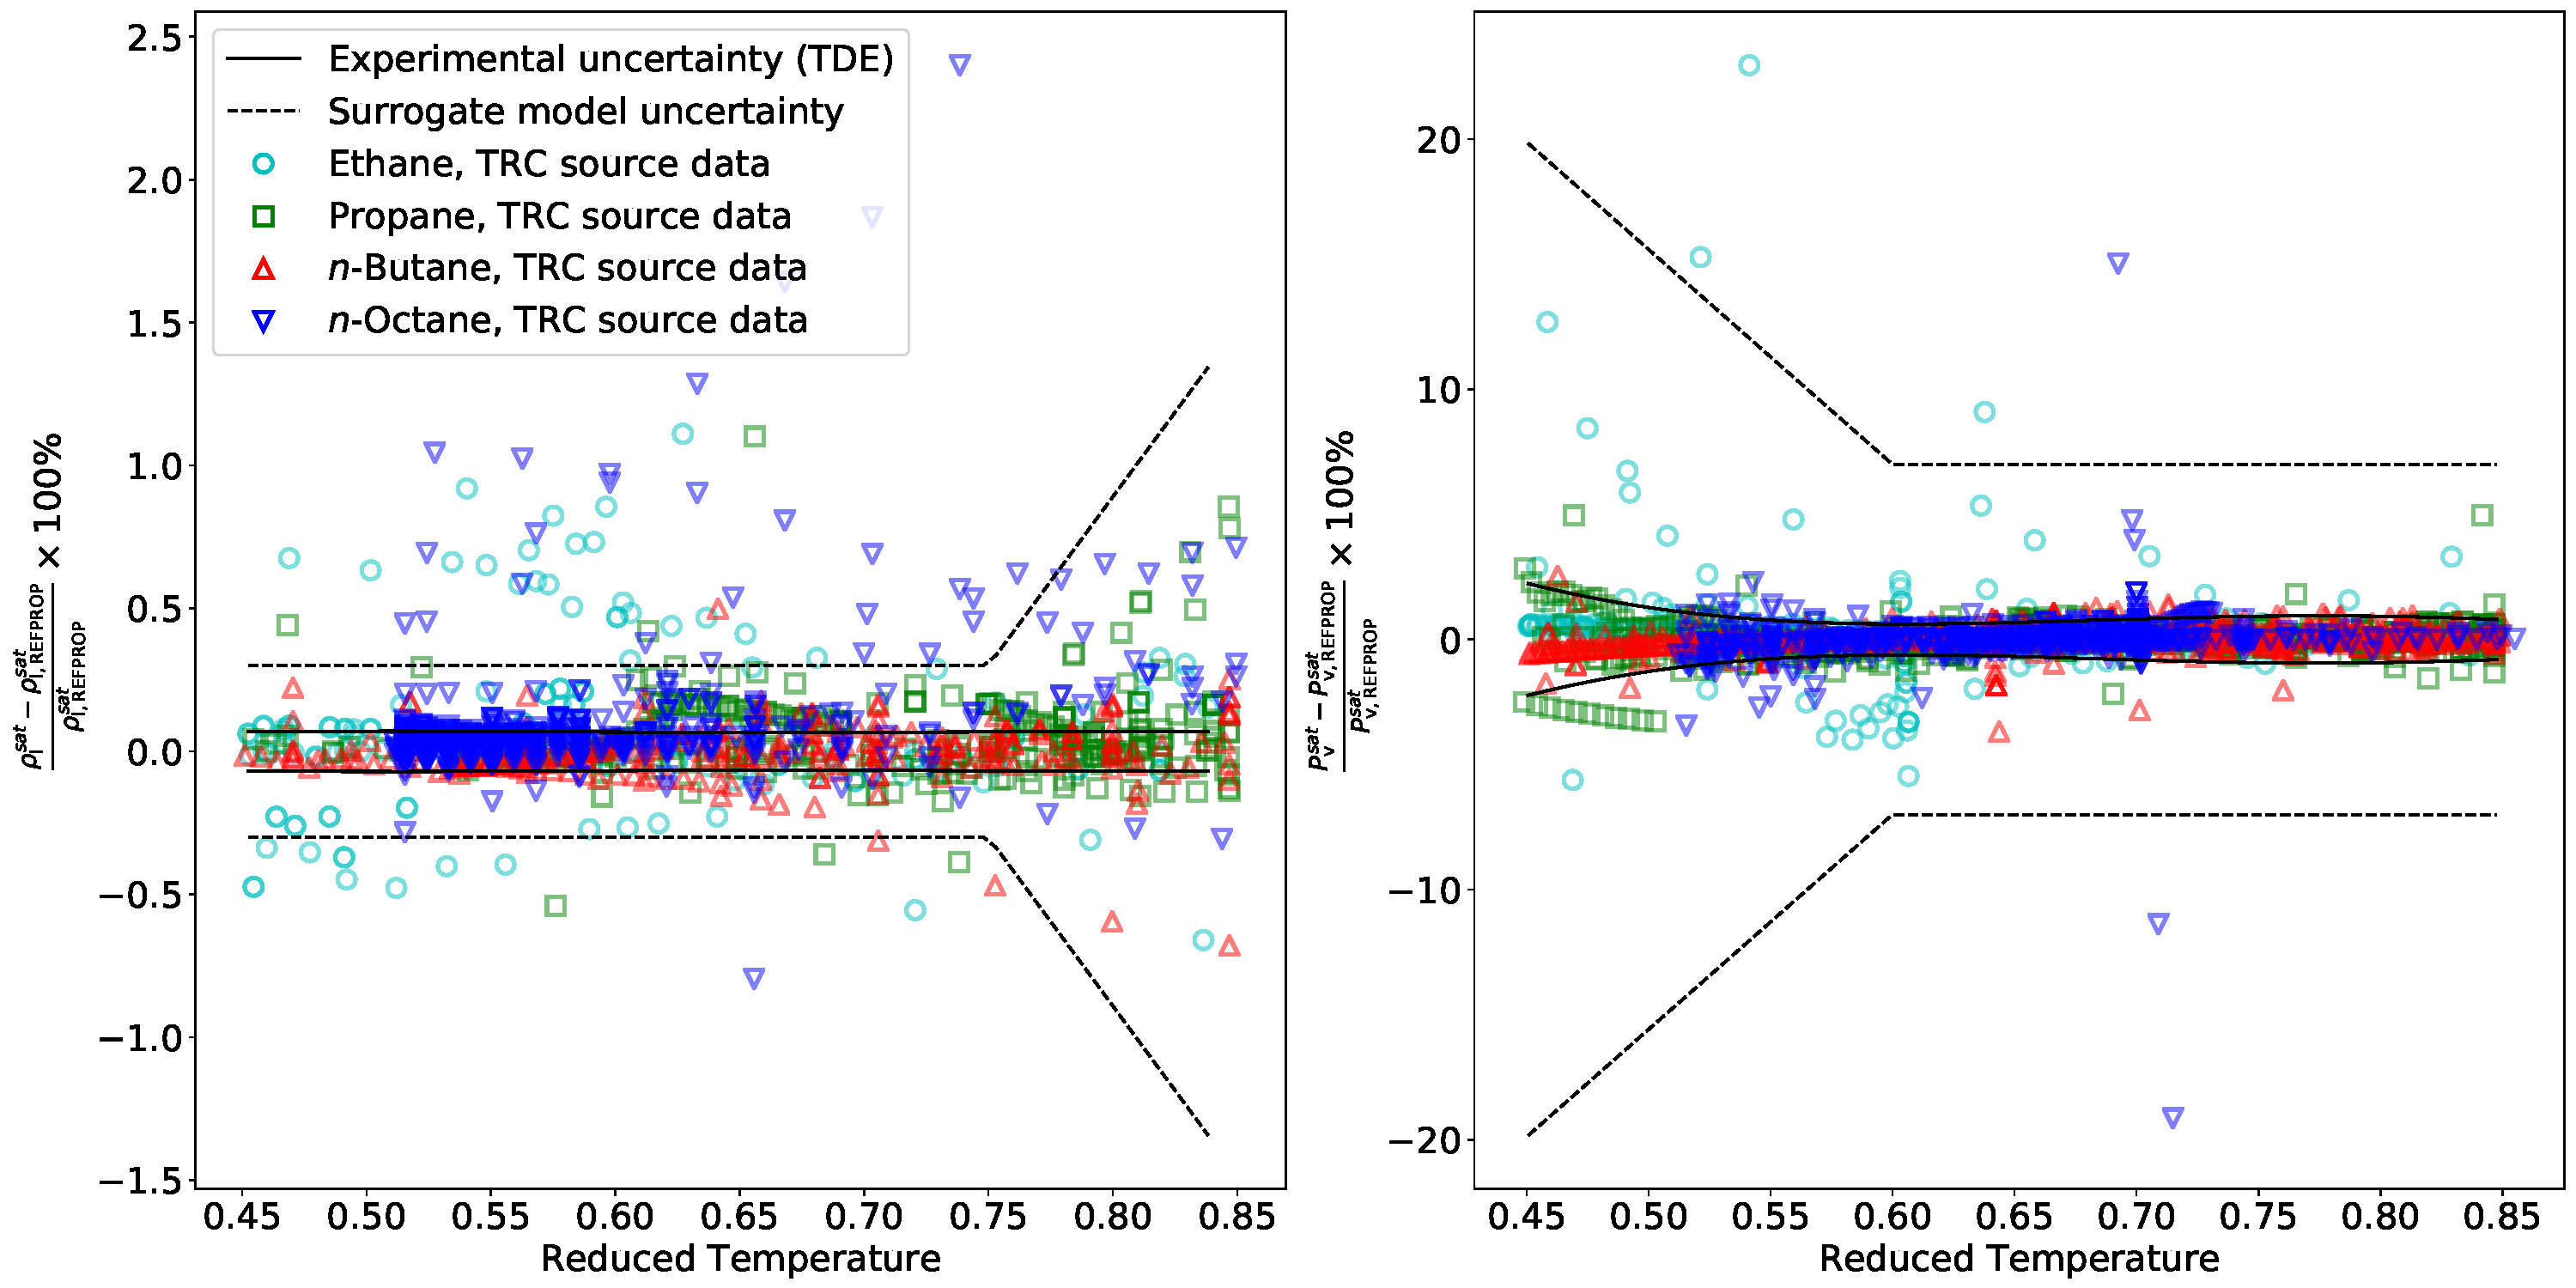
\includegraphics[width=6.4in]{Error_model_alkanes}
	\caption{Experimental (TDE) uncertainties are negligible compared to surrogate model uncertainties. Panels a)--b) plot the uncertainties for $\rho_{\rm l}^{\rm sat}$ and $P_{\rm v}^{\rm sat}$ with respect to reduced temperature (absolute temperature divided by the REFPROP $T_{\rm c}$). Also included are percent deviations between the experimental data for ethane, propane, \textit{n}-butane, and \textit{n}-octane relative to the REFPROP correlations.}
	\label{fig:Error_model}
\end{figure} 

%RAM2: Fixed some problems here
%The likelihood is calculated using a multi-variate normal distribution, $N(\mu, \Sigma)$, where $\mu$ are the experimental data values, and the covariance matrix $(\Sigma)$ accounts for the variances of both the experimental data and the surrogate model to estimate $\rho_{\rm l}^{\rm sat}$ and $P_{\rm v}^{\rm sat}$ for a given $\epsilon, \sigma$, and $\lambda$ (see Section \ref{Surrogate Model}). The variances 
%are assumed to be independent
%% such 
%meaning that the combined variance is the sum of the experimental and surrogate model variances \cite{Bay_MD}. The experimental data and corresponding variances were obtained through the Thermodynamics Research Center (TRC) ThermoData Engine (TDE) \cite{TDE}. The surrogate model variance is discussed in Section \ref{Surrogate Model}.
%MRS2: should be consistent on ``uncertainties'' and ``variances'' in preceeding paragraph.
%RAM2: Done


%\begin{enumerate}
%	\item By quantifying the uncertainty in epsilon and sigma for a given lambda, we can determine if the Mie potential is adequate for reproducing VLE and compressed liquid/supercritical pressures
%	\item Posterior includes saturated liquid density and vapor pressure
%	%%% RAM: Or should we compare several different posteriors? I.e. include rholsat and Pvsat, or rholsat and highP, or all three?
%        %%% MRS: which experiments to incldue are a design choice.  You either specify the experiments you require, or you could show which models are valid for predicting which proprerties.  
%	\item Markov Chain Monte Carlo is used to sample % RAM: Again, do we need to do MCMC or can we simplify things by just performing a 2-D scan
%	\item Details for MCMC are provided in supporting information (i.e. number of steps for burn-in and production, frequency that step sizes are updated, resulting acceptance percentages, etc.)
%	\item The parameter uncertainty is propagated when predicting high pressures
%	% RAM:  No longer finding the optimal lambda for high pressures \item To determine the optimal value of lambda for compressed liquid pressures, we redefine the posterior using only saturated liquid density and compressed liquid pressures  
%\end{enumerate}

\subsection{Surrogate Model} \label{Surrogate Model}

A typical Markov Chain requires $O(10^4$--$10^5)$ Monte Carlo steps, where the likelihood function must be evaluated at each step. Since $L(\theta|D,M)$ depends on the force field parameters $(\epsilon, \sigma, $ and $\lambda)$, an MCMC approach is computationally infeasible if computing $L(\theta|D,M)$ requires performing direct molecular simulations for every proposed parameter set. Furthermore, propagation of uncertainty with robust posterior prediction may require $O(10^2$--$10^3)$ $\theta_{\rm MCMC}$ parameter sets for adequate representations of $Pr(QoI|D,M)$ (see Equations \ref{Posterior Prediction} and \ref{Posterior Prediction Z}). For these reasons, surrogate models to estimate $\rho_{\rm l, MCMC}^{\rm sat}$, $P_{\rm v, MCMC}^{\rm sat}$ and $Z_{\rm MCMC}$ are essential for this study.

%Specifically, we implement surrogate models to estimate $\rho_{\rm l, MCMC}^{\rm sat}$, $P_{\rm v, MCMC}^{\rm sat}$ and $Z_{\rm MCMC}$. 

We use a configuration-sampling-based surrogate model, where configurations are sampled using a small group of reference parameter sets $(\epsilon_{\rm ref}, \sigma_{\rm ref}$, and $\lambda_{\rm ref})$ \cite{Postdoc_1}. As discussed in our previous study, we use a single value of $\epsilon_{\rm ref}$ with nine evenly spaced $\sigma_{\rm ref}$ values for a fixed value of $\lambda_{\rm ref} = \lambda$. Ensemble averages for the MCMC parameter sets $(\theta_{\rm MCMC})$ are estimated by reweighting the sampled reference configurations using Multistate Bennett Acceptance Ratio (MBAR) \cite{shirts-chodera:jcp:2008:mbar}. MBAR is a nearly exact surrogate model when there are a sufficient number of effective samples \cite{Postdoc_1}.

The properties that are estimated using MBAR are the departure internal energy $(U^{\rm dep})$ and the compressibility factor $(Z)$. 
%As discussed in Section \ref{Methods I}, 
Isothermal isochoric integration (ITIC) converts the MBAR estimated $U^{\rm dep}$ and $Z$ values at the 19 ITIC state points to saturation temperatures $(T^{\rm sat})$, saturated liquid densities $(\rho_{\rm l}^{\rm sat})$, saturated vapor densities $(\rho_{\rm v}^{\rm sat})$, and saturated vapor pressures $(P_{\rm v}^{\rm sat})$. This is important since $\rho_{\rm l}^{\rm sat}$ and $P_{\rm v}^{\rm sat}$ are the data $(D)$ included in $L(\theta|D)$. Details for the combined implementation of MBAR and ITIC (MBAR-ITIC) is discussed elsewhere \cite{Postdoc_1}. 

%The state points depicted in Figure \ref{fig:simulation_conditions} correspond to the recommended conditions for the isothermal isochoric integration (ITIC) algorithm \cite{Mostafa_Diss,Postdoc_1}. 
%ITIC converts the departure internal energies $(U^{\rm dep})$ and compressibility factors $(Z)$ obtained at the 19 state points to saturated VLE properties, namely, $\rho_{\rm l}^{\rm sat}$ and $P_{\rm v}^{\rm sat}$.
The 
%fundamental 
ITIC equations are: 
\begin{equation} \label{ITIC A}
\frac{A^{\rm dep}}{R_{\rm g}T^{\rm sat}} = \int_{0}^{\rho_{\rm l}^{\rm sat}}\frac{Z-1}{\rho} \partial \rho |_{T = T^{\rm IT}} + \int_{T^{\rm IT}}^{T^{\rm sat}}U^{\rm dep}\partial\left(\frac{1}{R_{\rm g}T}\right)|_{\rho=\rho_{\rm l}^{\rm sat}}
\end{equation}
\begin{equation} \label{ITIC rhov}
\rho_{\rm v}^{\rm sat} \approx \rho_{\rm l}^{\rm sat} \exp \left( \frac{A^{\rm dep}}{R_{\rm g}T^{\rm sat}} + Z_{\rm l}^{\rm sat} - 1 - 2 B_2 \rho_{\rm v}^{\rm sat} - 1.5 B_3 (\rho_{\rm v}^{\rm sat})^2 \right)
\end{equation}
\begin{equation} \label{ITIC Pv}
P_{\rm v}^{\rm sat} \approx \left(1 + B_2 \rho_{\rm v}^{\rm sat} + B_3 (\rho_{\rm v}^{\rm sat})^2\right)\rho_{\rm v}^{\rm sat} R_{\rm g}T^{\rm sat}
\end{equation}
\begin{equation} \label{ITIC Zl}
Z_{\rm l}^{\rm sat} = \frac{P_{\rm v}^{\rm sat}}{\rho_{\rm l}^{\rm sat} R_{\rm g} T^{\rm sat}}
\end{equation}
where $A^{\rm dep} \equiv A-A^{\rm ig}$ is the Helmholtz free energy departure from ideal gas for $T = T^{\rm sat}$ and $\rho = \rho_{\rm l}^{\rm sat}$, $U^{\rm dep} \equiv U-U^{\rm ig}$ is the internal energy departure, $Z_{\rm l}^{\rm sat}$ is the saturated liquid compressibility factor, $B_2$ is the second virial coefficient, $B_3$ is the third virial coefficient, $T^{\rm IT}$ is the isothermal temperature, and $R_{\rm g}$ is the universal gas constant. For details regarding the implementation of ITIC, see References \citenum{Postdoc_1,Mostafa_Diss,Mostafa2018}. As discussed in our previous work \cite{Postdoc_1}, the $B_2$ and $B_3$ values found in Equations \ref{ITIC rhov}-\ref{ITIC Pv} are calculated using REFPROP correlations \cite{LEMMON-RP91}. The use of REFPROP correlations introduces a small bias in the resulting $\rho_{\rm l}^{\rm sat}$ and $P_{\rm v}^{\rm sat}$, which is accounted for in the surrogate model uncertainty.

The ITIC analysis provides VLE properties at only 5 saturation temperature values $(T^{\rm sat}_{\rm ITIC})$, while the experimental data set may have hundreds of saturation temperatures $(T^{\rm sat}_{\rm D})$. Although it is possible to use computed values from an empirical correlation fit to experimental data (i.e. REFPROP, ThermoData Engine (TDE)) as the data set, it is considered best practice for Bayesian inference that $D$ consist of raw experimental data.
% are preferred when performing a Bayesian analysis. 
%MRS2: this is a bit unclear.  You are using fitting the Antoine equation to the simulated ITIC to compare to experiment? Maybe make it a bit clearer. Is that error incorporated (i.e. it's not ONE set of Antoine equation parameters, but a family?) 
%RAM2: I modified the previous line and tried to make this statement a little more clear
For this reason, we instead use empirical model fits to interpolate the ITIC VLE properties $(T^{\rm sat}_{\rm ITIC}$, $\rho_{\rm l, ITIC}^{\rm sat}$, and $(P_{\rm v, ITIC}^{\rm sat})$ so that $\rho_{\rm l}^{\rm sat}$ and $P_{\rm v}^{\rm sat}$ can be estimated at any value of $T^{\rm sat}$. Specifically, we fit $P_{\rm v, ITIC}^{\rm sat}$ and $T^{\rm sat}_{\rm ITIC}$ to the Antoine equation:
\begin{equation} \label{Antoine}
\log_{\rm 10}(P_{\rm v}^{\rm sat}) = a_0 + \frac{a_1}{T^{\rm sat} + a_2}
\end{equation}
where $a_i$ are fitting parameters.
We fit $\rho_{\rm l, ITIC}^{\rm sat}$ and $T^{\rm sat}_{\rm ITIC}$ to a combined rectilinear and density scaling law expression \cite{Mess4}:
\begin{equation} \label{Rectilinear Scale}
\rho_{\rm l}^{\rm sat} = b_0 + b_1 (b_2 - T^{\rm sat}) + b_3 (b_2 - T^{\rm sat}) ^ {\beta}
\end{equation}
where $b_i$ are fitting parameters, and $\beta = 0.326$. $b_0$ and $b_2$ only provide rough estimates of the critical density $(\rho_c)$ and critical temperature $(T_{\rm c})$. More reliable estimates of the critical point require simultaneous fitting of $\rho_{\rm v, ITIC}^{\rm sat}$ to a similar expression, but this is unnecessary for our purposes since $D$ does not include the critical constants. Note that Equations \ref{Antoine}-\ref{Rectilinear Scale} are only used to interpolate ITIC values, and not to extrapolate to higher or lower $T^{\rm sat}$. These equations are reliable over the limited temperature range studied $(0.45 < T_{\rm r} < 0.85)$, whereas a wider temperature range would require more flexible models \cite{Riedel,Funke}. 

In summary, MBAR, ITIC, and Equations \ref{Antoine}-\ref{Rectilinear Scale} enable prediction of $\rho_{\rm l}^{\rm sat}$ and $P_{\rm v}^{\rm sat}$ over a range of $T^{\rm sat}$ for any $\epsilon$, $\sigma$, and $\lambda$ by performing a small number of direct NVT simulations with only a few reference parameter sets. In addition, since the Mie $\lambda$-6 potential is linear with respect to $r^{-6}$ and $r^{-\lambda}$ (see Equation \ref{eq:Mie}), we implement basis functions to efficiently recompute the energies and forces that are required for MBAR and ITIC (for details see Reference \citenum{naden:jctc:2016} and Section SI.IV of Supporting Information in Reference \citenum{Postdoc_1}). 
%MRS2: also cite one of Levi's papers here.
%RAM2: Done
In total, this methodology reduces the computational cost for computing $L(\theta|D)$ by several orders of magnitude compared to direct simulation of VLE, using Gibbs Ensemble Monte Carlo (GEMC) or Grand Canonical Monte Carlo (GCMC) histogram reweighting (HR).

Quantifying the surrogate model variance $(s^2_{\rm SM})$ 
%, i.e. the standard deviation or variance due to the MBAR, ITIC, and Equations \ref{Antoine}-\ref{Rectilinear Scale} methodology, 
is essential for evaluating $L(\theta|D)$. While only a brief description is provided here, details are found in Section \ref{Error Model} of Supporting Information. Rather than performing a rigorous statistical assessment of MBAR, ITIC, and Equations \ref{Antoine}-\ref{Rectilinear Scale}, we use an empirical approach for estimating $s^2_{\rm SM}$. Specifically, we compute the deviation between the surrogate model estimates of $\rho_{\rm l}^{\rm sat}$ and $P_{\rm v}^{\rm sat}$ for TraPPE-UA and Potoff 
%MRS2: suggest being more explicit that all calculations are using the SAME model parameters, since that is key.
%RAM2: Done
with those reported in the literature for the respective force fields obtained using Gibbs Ensemble Monte Carlo (GEMC) or Grand Canonical Monte Carlo (GCMC) histogram reweighting (HR) \cite{TraPPE,Mie}. Although this is a rough approximation for estimating $s^2_{\rm SM}$, this inter-laboratory comparison has the added benefit that it incorporates possible ``dark uncertainty'' \cite{GUM}, which can be significant \cite{RoundRobin}. These non-statistical deviations are typically associated with different simulation packages, MD instead of MC, finite-size effects, and post-simulation analysis (e.g. ITIC rather than HR).
%MRS3: Might also make it clear that THESE sources of error are greater than the MBAR error, hence why it's neglected.
%RAM3: True. I do not want to imply that our uncertainties should be attributed to MBAR or ITIC. I have tried to say that by emphasizing that these are conservative estimates, but I could probably say something more here.

%%%RAM2: Moved to implementation section
%As shown in Figure \ref{fig:Error_model}, the surrogate model uncertainty $(u_{\rm SM}$, reported at the 95\% confidence level) for $\rho_{\rm l}^{\rm sat}$ is 0.3\% up to $0.75 T_{\rm c}$ and increases linearly to 1.5\% at the maximum $T^{\rm sat}$. The surrogate model uncertainty for $P_{\rm v}^{\rm sat}$ is 20\% at the minimum $T_{\rm sat}$ and decreases linearly to 7\% at $0.6 T_{\rm c}$, where it remains constant for higher temperatures. Note that these are conservative estimates of $u_{\rm SM}$, where other studies suggest ITIC can have significantly smaller uncertainties \cite{Mostafa_Diss}. In fact, for the compounds investigated in this study, these uncertainties are much larger than the experimental uncertainties $(u_{\rm D})$ and, therefore, the size of the parameter space sampled by MCMC depends almost entirely on $u_{\rm SM}$. The use of a conservative $u_{\rm SM}$ model is intentional in this regard, namely, so that the $\theta_{\rm MCMC}$ sampled points represent practically all of the feasible values of $\epsilon$ and $\sigma$ for optimizing $\rho_{\rm l}^{\rm sat}$ and $P_{\rm v}^{\rm sat}$. 


%Quantifying the surrogate model uncertainty $(u_{\rm SM})$ 
%%, i.e. the standard deviation or variance due to the MBAR, ITIC, and Equations \ref{Antoine}-\ref{Rectilinear Scale} methodology, 
%is essential for evaluating $L(\theta|D)$. Rather than performing a rigorous statistical assessment of MBAR, ITIC, and Equations \ref{Antoine}-\ref{Rectilinear Scale}, we use an empirical approach for estimating the surrogate model uncertainty. Specifically, we compute the percent deviation between the surrogate model estimates for $\rho_{\rm l}^{\rm sat}$ and $P_{\rm v}^{\rm sat}$ values for TraPPE and Potoff 
%%MRS2: suggest being more explicit that all calculations are using the SAME model parameters, since that is key.
%%RAM2: Done
%with those reported in the literature for the respective force fields obtained using Gibbs Ensemble Monte Carlo (GEMC) or Grand Canonical Monte Carlo (GCMC) histogram reweighting (HR). Although this is a rough approximation for estimating uncertainties, this comparison has the added benefit that it incorporates possible deviations associated with the simulation package, and post-simulation analysis, which can be significant \cite{RoundRobin}.
%
%The surrogate model uncertainty for $\rho_{\rm l}^{\rm sat}$ is 0.3\% up to $0.75 T_{\rm c}$ and increases linearly to 1.5\% at the maximum $T^{\rm sat}$. The surrogate model uncertainty for $P_{\rm v}^{\rm sat}$ is 20\% at the minimum $T_{\rm sat}$ and decreases linearly to 7\% at $0.6 T_{\rm c}$, where it remains constant for higher temperatures. Note that these are conservative estimates of $u_{\rm SM}$, where other studies suggest ITIC can have significantly smaller uncertainties \cite{Mostafa_Diss}. In fact, for the compounds investigated in this study, these uncertainties are much larger than the experimental uncertainties $(u_{\rm D})$ and, therefore, the size of the parameter space sampled by MCMC depends almost entirely on $u_{\rm SM}$. The use of a conservative $u_{\rm SM}$ model is intentional in this regard, namely, so that the $\theta_{\rm MCMC}$ sampled points represent the only feasible values of $\epsilon$ and $\sigma$ for optimizing $\rho_{\rm l}^{\rm sat}$ and $P_{\rm v}^{\rm sat}$. Figure \ref{fig:Error_model} demonstrates that the experimental uncertainties are negligible compared to the surrogate model uncertainties for $\rho_{\rm l}^{\rm sat}$ and $P_{\rm v}^{\rm sat}$.
%
%\begin{figure}[htb!]
%	\centering
%	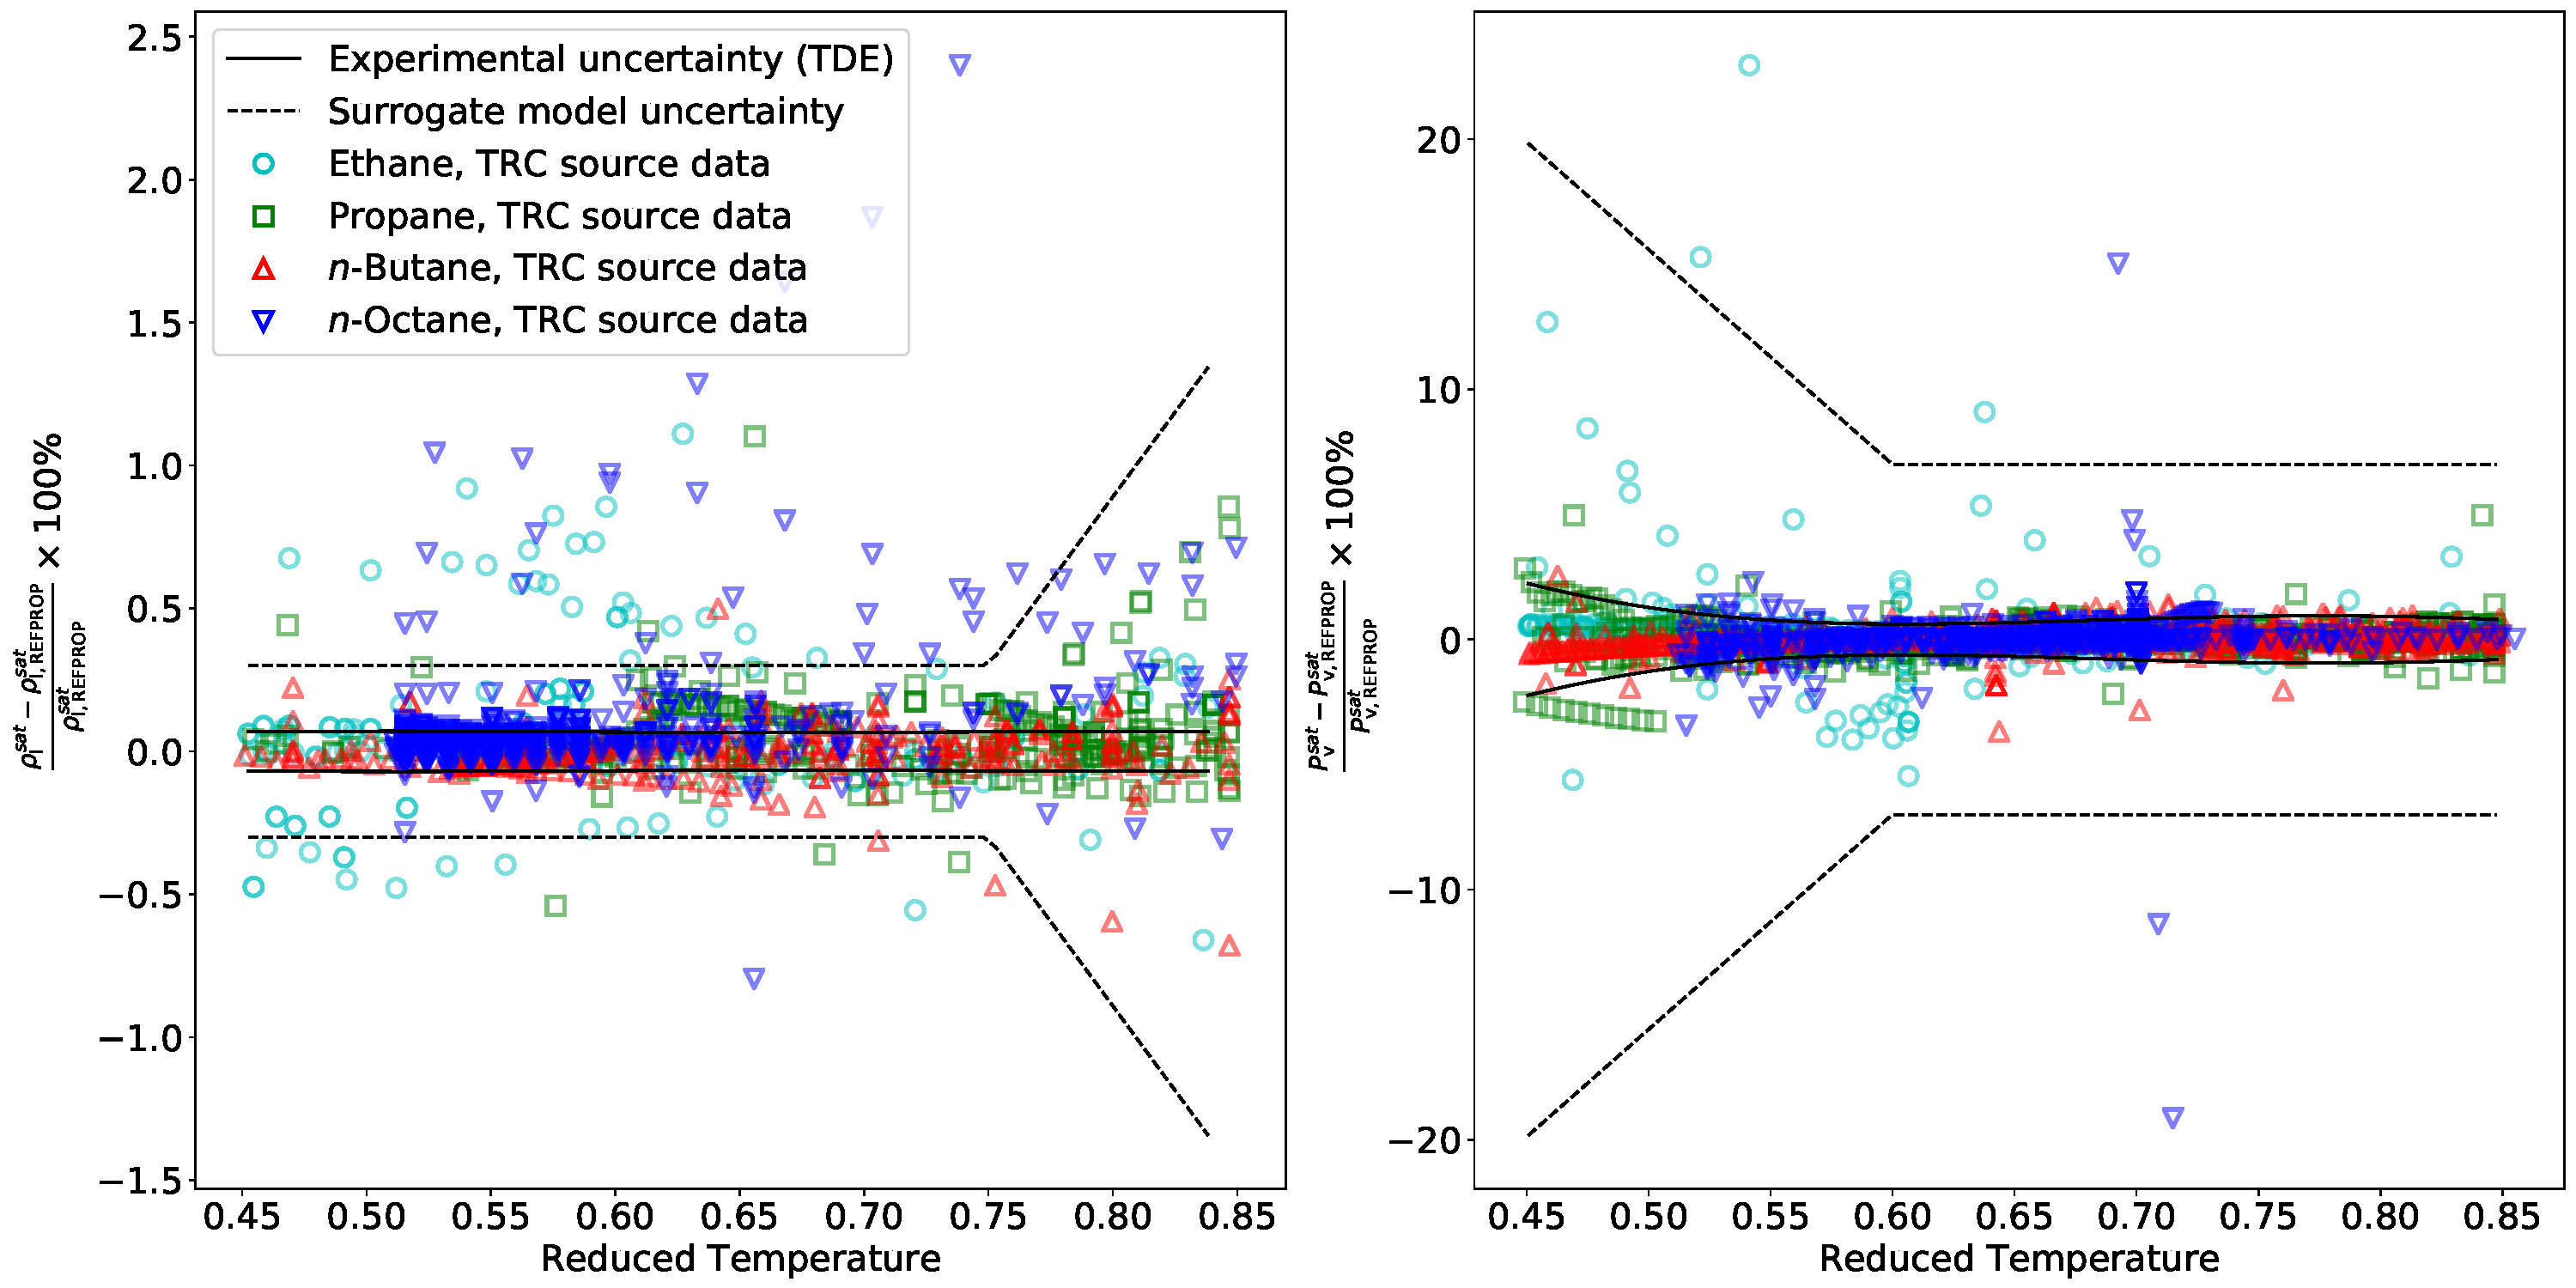
\includegraphics[width=6.4in]{Error_model_alkanes}
%	\caption{Surrogate model uncertainties are larger than experimental (TDE) uncertainties by at least a factor of five. Panel a) and b) plot the uncertainties for $\rho_{\rm l}^{\rm sat}$ and $P_{\rm v}^{\rm sat}$ with respect to reduced temperature (absolute temperature divided by the REFPROP $T_{\rm c}$). Also included are percent deviations between the experimental data for ethane, propane, \textit{n}-butane, and \textit{n}-octane relative to the REFPROP correlations.}
%	\label{fig:Error_model}
%\end{figure} 

%for any experimental saturation temperature $(T^{\rm sat}_{\rm exp})$. 
%
%Since the data $(D)$ included in $L(\theta|D)$ are saturated liquid densities $(\rho_{\rm l}^{\rm sat})$ and vapor pressures $(P_{\rm v}^{\rm sat})$, Isothermal Isochoric Integration (ITIC) converts $U^{\rm dep}$ and $Z$ to $\rho_{\rm l}^{\rm sat}$ and $P_{\rm v}^{\rm sat}$.
%
% There are three layers for the surrogate model implemented in this study: Multistate Bennett Acceptance Ratio, Isothermal Isochoric Integration, and Empirical Correlations. The fundamental layer, Multistate Bennett Acceptance Ratio (MBAR), reweights configurations that are sampled from a set of reference parameter sets $(\epsilon_{\rm ref}, \sigma_{\rm ref})$ 
%
%\begin{enumerate}
%	\item A Bayesian analysis is computationally too expensive if direct molecular simulations are performed for every MCMC step
%	\item As demonstrated in a previous publication, MBAR can reweight the configurations that are sampled from different force fields without direct simulation
%	\item In other words, a set of reference force fields are simulated for each molecule and MBAR is used instead of direct simulation for each MCMC step
%	\item As demonstrated in a previous publication, MBAR is used to predict Udep and Z while ITIC is used to convert Udep and Z to rholsat and Pvsat
%	\item ITIC state points are fit to rectilinear and Antoine equation to interpolate rholsat and Pvsat, this allows for comparison with experimental data at hundreds of temperatures
%	\item The likelihood includes the experimental uncertainties but, more importantly, the numerical uncertainties. In other words, the numerical uncertainties account for the uncertainties that arise from the simulations themselves, the MBAR reweighting, the ITIC algorithm, and fitting to rectilinear and Antoine.
%	\item To leave no room for doubt in our conclusions, we use very conservative (and empirical) estimates of numerical uncertainty for rholsat and Pvsat (see Supporting Information)
%\end{enumerate}

%\subsection{Propagation of Uncertainty}
%%RAM: I think we should move this inside the Bayesian analysis section.
%%MRS: not sure what you mean by propagation of uncertainty here. Uncertainty in credible region? 
%\begin{enumerate}
%	\item From the MCMC parameter sets, we randomly sample a subset of 100-1000 parameter sets
%	\item We use MBAR to predict Z for each of those parameter sets
%	\item We plot these results as a histogram to determine the 95\% credible interval for Z at each state point
%\end{enumerate}

\section{Results} \label{Results}

%\subsection{VLE and Compressed}

%\subsection{Parameter uncertainties}

%CH3 Results:
%
%Figure: Ethane CH3 uncertainties. Panel a) 14-6, 15-6, 16-6. Panel b) Z plots for each exponent
%Figure: Evidence for 14-6, 15-6, 16-6 based on VLE
%
%CH2 results:
%
%Combine these into one figure
%Figure: CH2 uncertainties. Panel a) 16-6 Panel b) 14-6

%MRS2: how hard would it be to do the full 4 parameter model?  I'm guessing it's because doing all the basis functions is harder?  Maybe be more explicit as to 1) the cost and 2) why you think it doesn't matter (i.e. it's OK to force the other models to use ethane parameters).  From my perspective, the difference between the 4 parameter and 2,2 parameter model is extremely interesting and may show us when we get results we don't expect. 
%RAM2: It would not be too difficult, but I don't think it is necessary considering the primary purpose of this text. 
In this section, we use MCMC and the aforementioned surrogate models to determine the parameter uncertainty in CH$_3$ and CH$_2$ interaction sites of \textit{n}-alkanes. Since the common practice is to limit $\lambda$ to integer values (see Section \ref{Force Field}), we perform several independent MCMC runs using a single, fixed, integer value of $\lambda$. The Bayesian inference analysis for CH$_3$ and CH$_2$ sites is performed sequentially. Specifically, rather than sampling from a four-dimensional parameter space (i.e. $\epsilon_{\rm CH_3}$, $\epsilon_{\rm CH_2}$, $\sigma_{\rm CH_3}$, and $\sigma_{\rm CH_2}$ for a given value of $\lambda_{\rm CH_3}$ and $\lambda_{\rm CH_2}$), we implement a pair of two-dimensional MCMC runs by assuming the CH$_3$ parameters from ethane are transferable to propane, \textit{n}-butane, and \textit{n}-octane. 
%MRS3: may need to remind people later that this second run is done, and that it's done with fixed CH3.  That gets a little lost later in the paper. 
%RAM3: OK. I will try to make that clear later on.

%As mentioned in Section \ref{Force Field}, it is common to limit $\lambda$ to integer values. 
%MRS2: Is the next section needed?  If there are only a few choices of lambda that are reasonable, just treating them as separate models seems to be fine. You don't need to justify not doing MCMC between models, I don't think.
%RAM2: Hopefully the new version is clearer
%Due to the strong correlation between $\epsilon$ and $\lambda$, advanced sampling methods would be required to achieve good acceptance ratios when sampling from discrete values of $\lambda$. For this reason, we perform several independent MCMC runs using fixed values of $\lambda$. This approach is computationally more efficient since we are only concerned with a few values of $\lambda$ (i.e. $12$-$18$).    
%MRS2: the only thing that is needed if you can't jump between lambda-labeled distributions/models is explicitly calculate the normalizing constant between them, which I think you can do with explicit integration (though we will need to check that is done correctly).  I think it should be P(lambda|D)?
%RAM2: This is what we do to compute the Bayes factor
\subsection{Ethane} \label{Ethane}

%MRS2: here's a thought.  I think most of this paragraph actually should go in the caption (it should still start with a thesis sentence!). Right now, the figure isn't self contained.  I think it would read smoother if the TEXT focused on interpretationand analysis of the figures (what does it mean?) and the caption focused on what the data was. 
%RAM2: I agree. Most of this was originally in the caption, but I have been trying to shorten my figure captions.

%Figure \ref{fig:MCMC_Mie_13_14_15_16_17_18_ethane} presents the MCMC results for ethane with $\lambda_{\rm CH_3} =13$-$18$. Panel a) in Figure \ref{fig:MCMC_Mie_13_14_15_16_17_18_ethane} demonstrates that the feasible region of $\epsilon_{\rm CH_3}$ depends strongly on $\lambda_{\rm CH_3}$, namely, larger values of $\lambda_{\rm CH_3}$ require larger values of $\epsilon_{\rm CH_3}$. By contrast, we observe a much smaller shift towards larger values of $\sigma_{\rm CH_3}$ with increasing $\lambda_{\rm CH_3}$. This observation is consistent with the literature \cite{Mie}.

%Figure \ref{fig:MCMC_Mie_13_14_15_16_17_18_ethane} presents the MCMC results for ethane with $\lambda_{\rm CH_3} =13$-$18$. Panel a) plots the MCMC sampled parameter sets for different values of $\lambda_{\rm CH_3}$ ($\epsilon_{\rm CH_3, MCMC}$ and $\sigma_{\rm CH_3, MCMC}$). The inset of Panel a) plots the mean absolute percent deviation (MAPD\%) of the MCMC predicted VLE properties ($\rho_{\rm l, MCMC}^{\rm sat}$ and $P_{\rm v, MCMC}^{\rm sat}$). Panels b) and d) plot the percent deviation from REFPROP correlations for $\rho_{\rm l, MCMC}^{\rm sat}$ and $P_{\rm v, MCMC}^{\rm sat}$, respectively. Specifically, the upper and lower lines correspond to the uncertainty for each $\lambda$, which are determined at the 95\% credible level. The insets of Panels b) and d) are histograms of the MAPD\% in $\rho_{\rm l, MCMC}^{\rm sat}$ and $P_{\rm v, MCMC}^{\rm sat}$, respectively. Panel c) plots $Z$ with respect to inverse temperature for the two highest isochores $(\rho_0$ and $\rho_1$ in Panel a) of Figure \ref{fig:IC_normal_alkanes}). The inset of Panel c) plots the distribution of average deviation (AD\%) in pressure for the two highest densities along the supercritical isotherm $(P^{\rm high})$. The AD\% is chosen to demonstrate the positive bias in $P^{\rm high}$, while the MAPD\% is used when quantifying the goodness of fit in VLE data.
%MRS2: I'm having a hard time processing the entire figure, since it really is 8 figures in one.   Is there a good way to split it into 2? Obvously b and d go together well.  Perhaps a and c should be a separate figure? Too much information in too small a space.
%RAM2: I was considering this also. I combined this all into one figure because all of the data are closely related.
%Panel a) plots the MCMC sampled $\epsilon_{\rm CH_2}$ and $\sigma_{\rm CH_2}$ parameter sets for the different values of $\lambda_{\rm CH_3}$. The inset of Panel a) plots the AD\% of $\rho_{\rm l, MCMC}^{\rm sat}$ and $P_{\rm v, MCMC}^{\rm sat}$. Panels b) and d) plot the percent deviation from REFPROP correlations for $\rho_{\rm l, MCMC}^{\rm sat}$ and $P_{\rm v, MCMC}^{\rm sat}$, respectively. The insets of Panels b) and d) are histograms of the MCMC sampled distribution of AD\% for $\rho_{\rm l, MCMC}^{\rm sat}$ and $P_{\rm v, MCMC}^{\rm sat}$, respectively. Panel c) plots $Z$ with respect to inverse temperature for the two highest isochores $(\rho_0$ and $\rho_1$ in Panel a) of Figure \ref{fig:IC_normal_alkanes}). The inset of Panel c) plots the distribution of AD\% in pressure for the two highest densities along the supercritical isotherm $(P^{\rm high})$.

   
   %%%%% This is what I previously had when the Pareto front was an inset 
%
%\begin{figure}[p!]
%	\centering
%	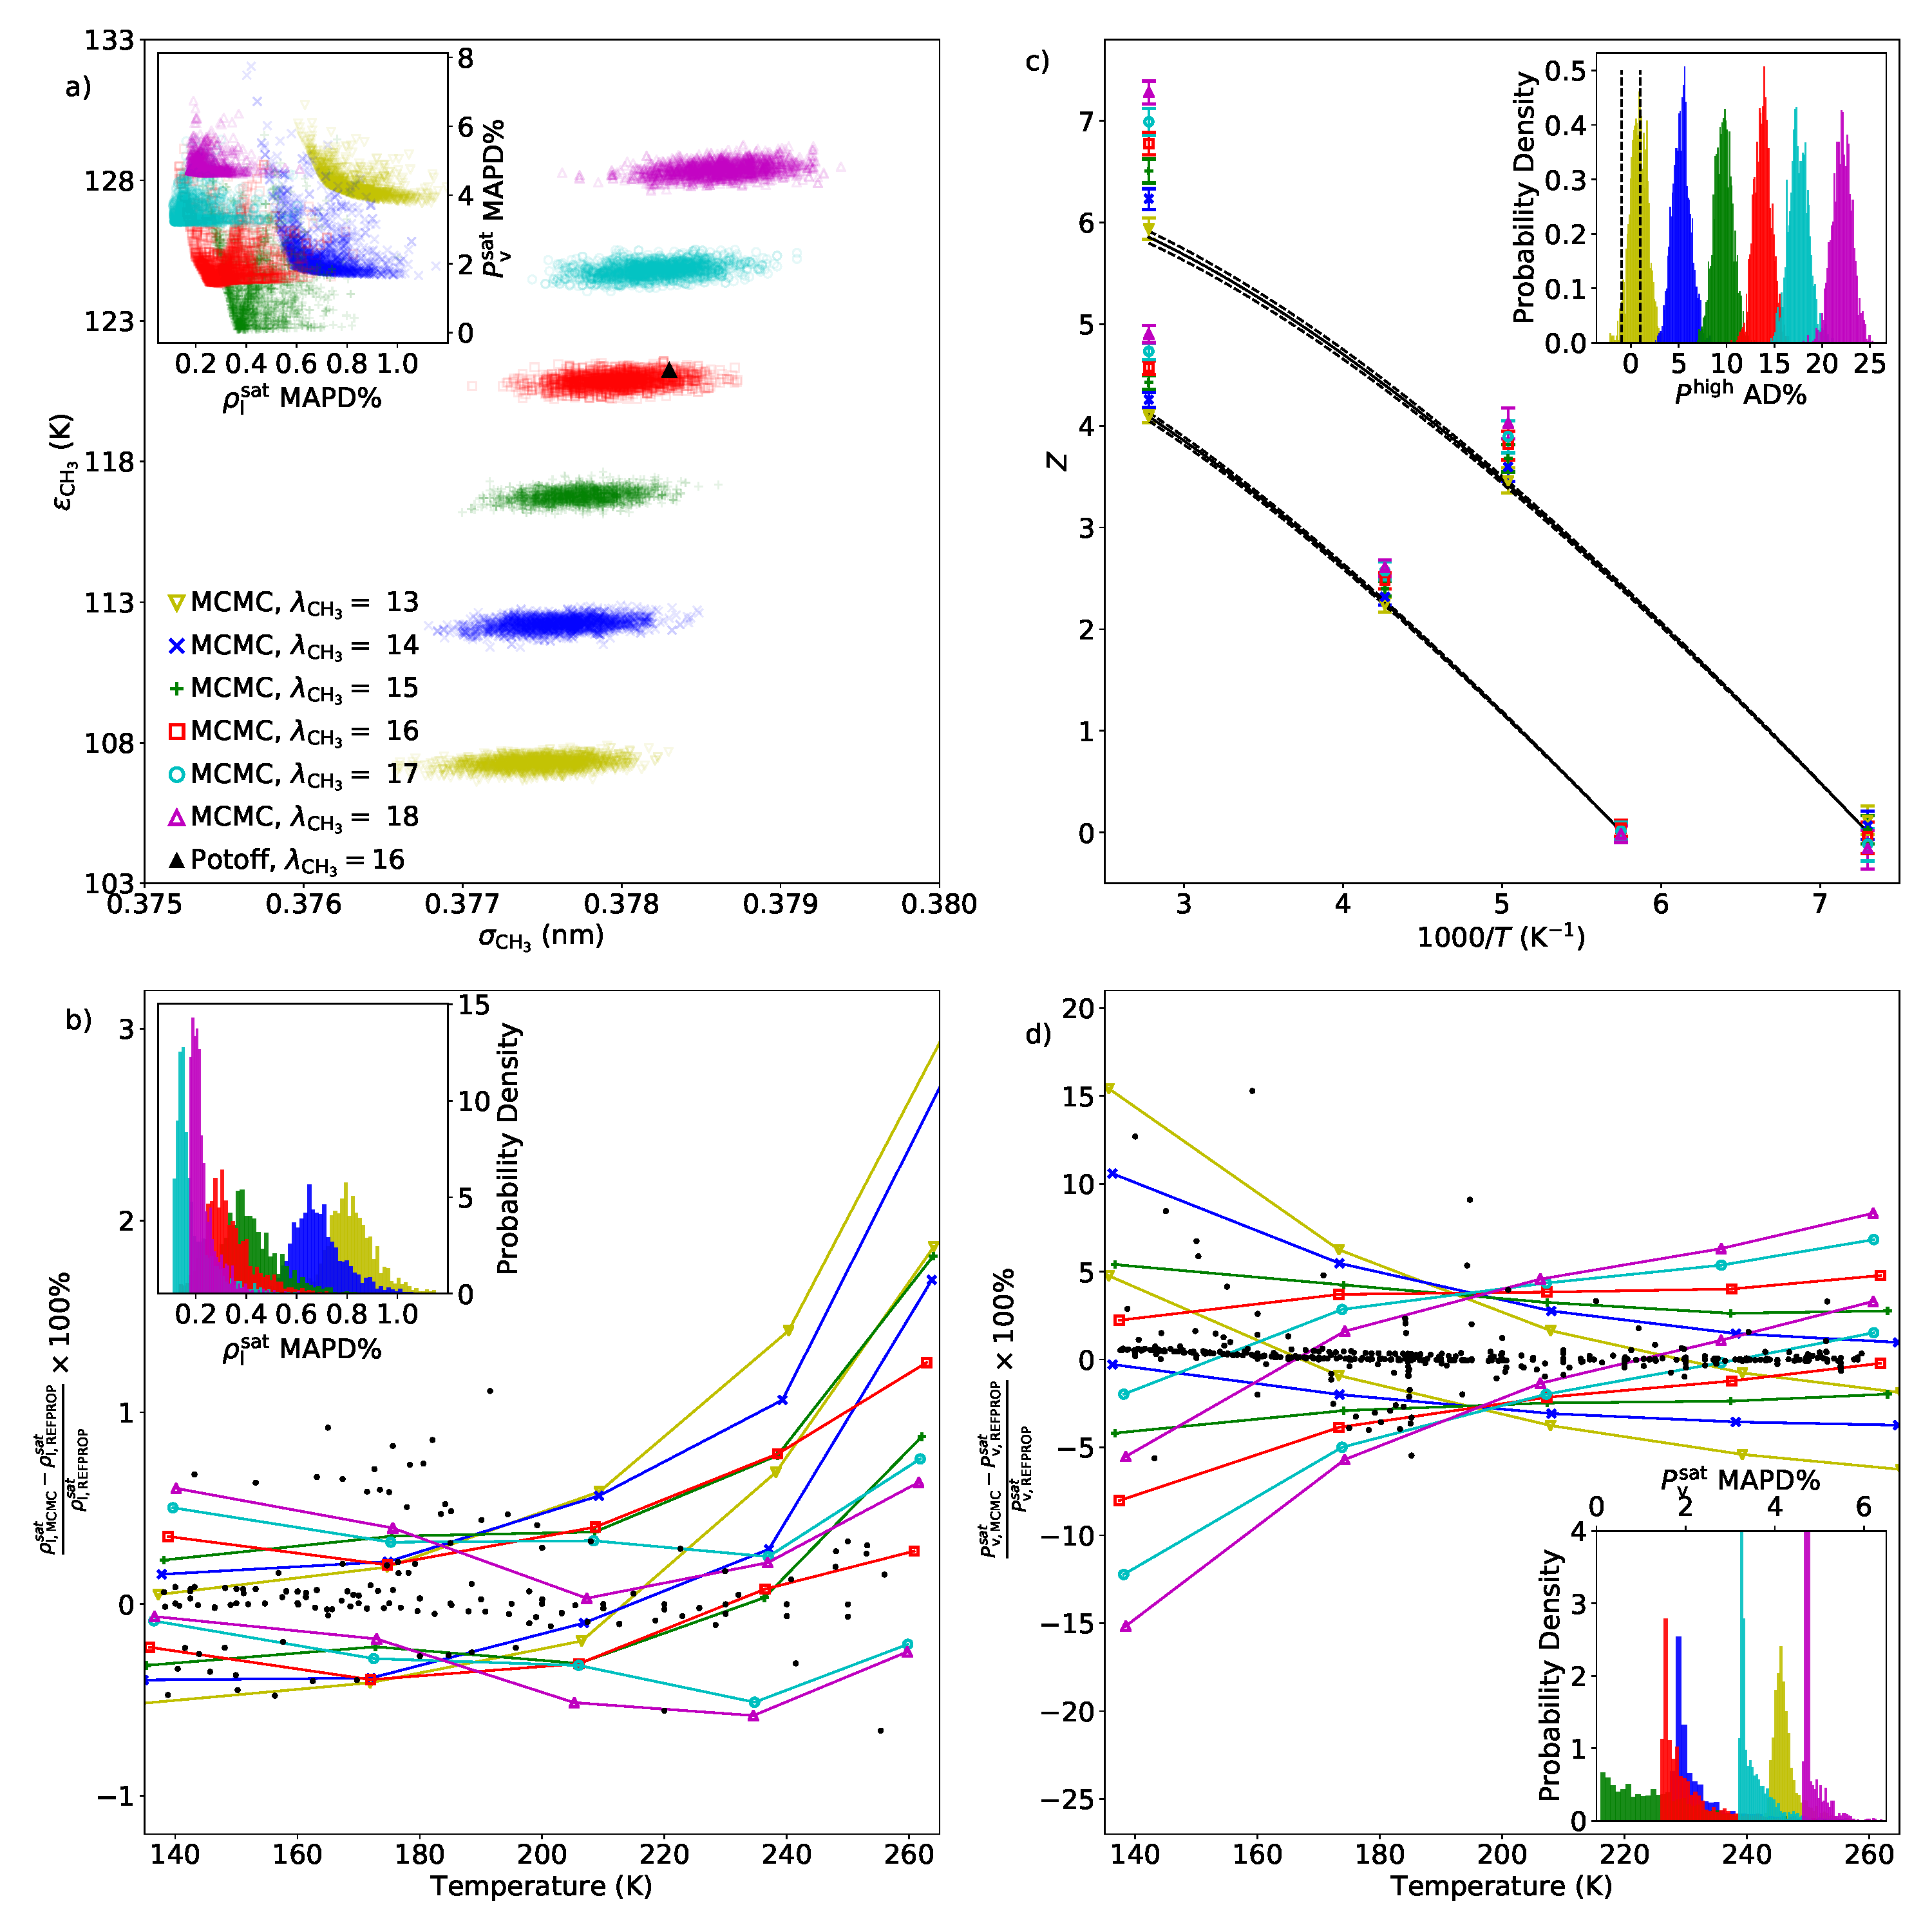
\includegraphics[width=6.1in]{MCMC_Mie_13_14_15_16_17_18_ethane}
%	\caption{MCMC results confirm that the UA Mie $\lambda$-6 potential cannot adequately predict both VLE and high pressures for supercritical fluids and compressed liquids. Panel a) plots the MCMC sampled parameter sets for different values of $\lambda_{\rm CH_3}$ ($\epsilon_{\rm CH_3, MCMC}$ and $\sigma_{\rm CH_3, MCMC}$) and the Potoff parameter set as a reference. Inset of Panel a) plots the mean absolute percent deviation (MAPD\%) of $\rho_{\rm l, MCMC}^{\rm sat}$ and $P_{\rm v, MCMC}^{\rm sat}$. Panels b) and d) plot the percent deviation from REFPROP correlations for $\rho_{\rm l, MCMC}^{\rm sat}$ and $P_{\rm v, MCMC}^{\rm sat}$, respectively, where the upper and lower lines correspond to the 95\% credible level for each $\lambda$. Insets of Panels b) and d) are histograms of the MAPD\% in $\rho_{\rm l, MCMC}^{\rm sat}$ and $P_{\rm v, MCMC}^{\rm sat}$, respectively. Experimental data used to compute the likelihood are included in Panels b) and d) as black dots. Panel c) plots $Z$ with respect to inverse temperature for the two highest isochore densities $(\rho_3$ and $\rho_4)$. Inset of Panel c) plots the distribution of average deviation (AD\%) in $P^{\rm high}$, i.e. pressure for $\rho_3$--$\rho_4$ and $T = T^{\rm IT}$. REFPROP uncertainty in $P^{\rm high}$ is $\pm 1$\%.}
%%MRS2: is the spread in exprimental data at each T the experimental uncertainty? I'm not entirely sure only one property is being predicted, meaning the spread is noise in a single obserbable.
%%RAM2: The experimental data are just included to give a sense for the goodness of fit. Is your point that I should not include them? 
%	\label{fig:MCMC_Mie_13_14_15_16_17_18_ethane}
%\end{figure} 
%
%% in Panel a) of Figure \ref{fig:IC_normal_alkanes})
%
%%MRS: suggest breaking up important points to separate paragraphs.
%
%The results depicted in Figure \ref{fig:MCMC_Mie_13_14_15_16_17_18_ethane} are useful for comparing the performance of different values of $\lambda$. Notice that the insets in Panels a), b), and d) plot the mean absolute percent deviation (MAPD\%) to quantify the goodness of fit to VLE data, while the inset in Panel c) plots the average deviation (AD\%) to demonstrate the positive bias in $P^{\rm high}$. Note that MAPD\% and AD\% are not directly related to the posterior distribution since our likelihood is a normal distribution, which is based on the squared deviations, while MAPD\% and AD\% are percent deviations. However, we plot MAPD\% and AD\% as these are easier to conceptualize and quantify. 
%
%Panel b) with the corresponding inset demonstrates that the best prediction of $\rho_{\rm l}^{\rm sat}$ is obtained for higher values of $\lambda_{\rm CH_3}$. However, while the $\rho_{\rm l}^{\rm sat}$ MAPD\% for $\lambda_{\rm CH_3} = 15$--$18$ are similar, $\lambda_{\rm CH_3} = 13$--$14$ have significantly higher $\rho_{\rm l}^{\rm sat}$ MAPD\%. 
%
%Panel d) demonstrates that $\lambda_{\rm CH_3} = 13$--$14$ and $\lambda_{\rm CH_3} = 17$--$18$ over- and under-predict $P_{\rm v}^{\rm sat}$ at low temperatures, respectively, 
%%MRS2: eyeballing, 14 looks consistent to me.  What quantitive measure can you use for what it means to over or underpredict?
%%RAM2: The MAPD histogram is intended to quantify this statement. Also, I just realized that I had an error in panels b,c, and d. Specifically, the errorbars and uncertainty regions represented the estimated 100% confidence region, i.e. all of the MCMC sampled values. I have now converted these to the 95% credible regions by integrating the histograms with equal areas. The results are much more conclusive now.
%while $\lambda_{\rm CH_3} = 15$--$16$ are the most reliable. $\lambda_{\rm CH_3} = 15$ has the least amount of bias and the lowest MAPD\% in $P_{\rm v}^{\rm sat}$ (see inset). 
%
%The inset of Panel a), helps to visualize the overall performance of different values of $\lambda_{\rm CH_3}$. 
%%MRS2: be more precise about noticing the pareto front.  You mean in Panel a?) Can you draw a line indicating it? Some people might not have a sense of what they would be looking for.
%Notice the trade-off between the MAPD\% of $\rho_{\rm l}^{\rm sat}$ and $P_{\rm v}^{\rm sat}$. This compromise between two competing properties included in the objective function, namely, $\rho_{\rm l}^{\rm sat}$ and $P_{\rm v}^{\rm sat}$, is known as a Pareto front \cite{Pareto_Deriv,Pareto_LJPQ,Pareto_ST}. The optimal location for a Pareto front is the bottom left region of the plot (low MAPD\% for both $\rho_{\rm l}^{\rm sat}$ and $P_{\rm v}^{\rm sat}$) while the worst location is the top right region (high MAPD\% for both $\rho_{\rm l}^{\rm sat}$ and $P_{\rm v}^{\rm sat}$). Note that the inset of Panel a) includes an approximate ``overall'' Pareto front that combines the results for all values of $\lambda_{\rm CH_3}$. Although not depicted for visual clarity, the ``L'' shaped frontier for different colors/symbols demonstrates that each $\lambda_{\rm CH_3}$ value also has its own Pareto front. Because the overall Pareto front consists of points from the $\lambda_{\rm CH_3} = 15$--$17$ Pareto fronts, the Pareto optimal $\lambda_{\rm CH_3}$ value is either $15$, $16$, or $17$, depending on the relative weight assigned to $\rho_{\rm l}^{\rm sat}$ and $P_{\rm v}^{\rm sat}$. By contrast, since the $\lambda_{\rm CH_3} = 13$, $14$, and $18$ Pareto fronts are completely inside the overall Pareto front, these $\lambda_{\rm CH_3}$ values are not optimal, regardless of the weighting.   
%
%% By comparing the Pareto fronts for different values of $\lambda_{\rm CH_3}$ with the overall Pareto front, $\lambda_{\rm CH_3} = 15$, $16$, or $17$ are the optimal choices, depending on the relative weight assigned to $\rho_{\rm l}^{\rm sat}$ and $P_{\rm v}^{\rm sat}$. The $\lambda_{\rm CH_3} = 13$, $14$, and $18$ Pareto fronts are completely inside the overall Pareto front, suggesting that these values are not optimal, regardless of the weighting assignment.
%
%% A Pareto front represents a compromise between the MAPD\% of $\rho_{\rm l}^{\rm sat}$ and $P_{\rm v}^{\rm sat}$ two competing contributions to the objective function. 
%
%%Notice the trade-off, i.e. the Pareto front, between the two properties included in the objective function, namely, $\rho_{\rm l}^{\rm sat}$ and $P_{\rm v}^{\rm sat}$ \cite{Pareto_Deriv,Pareto_LJPQ,Pareto_ST}. A Pareto front represents a compromise between the MAPD\% of $\rho_{\rm l}^{\rm sat}$ and $P_{\rm v}^{\rm sat}$ two competing contributions to the objective function. 
%
%%Consistent with the insets of Panels b) and d), the 15-6 potential has the lowest MAPD\% in $P_{\rm v}^{\rm sat}$, while the 16-6, 17-6, and 18-6 have slightly lower MAPD\% in $\rho_{\rm l}^{\rm sat}$ and the 13-6 and 14-6 have significantly higher MAPD for $\rho_{\rm l}^{\rm sat}$.
%
%Finally, and most importantly for our purposes, Panel c) demonstrates that all of the sampled $\epsilon_{\rm CH_3, MCMC}$ and $\sigma_{\rm CH_3, MCMC}$ parameter sets for $\lambda_{\rm CH_3} \ge 14$ over-predict $Z$ at high temperatures and densities $(P^{\rm high})$. As expected, the larger the value of $\lambda_{\rm CH_3}$, the 
%more 
%%greater 
%the force field over-predicts $P^{\rm high}$. For example, although $\lambda_{\rm CH_3} = 15$ and $16$ are the best values based on VLE data, they over-predict $P^{\rm high}$ by around 10 and 15\%, respectively. This supports the fundamental claim of this work, namely, that the UA Mie $\lambda$-6 potential cannot adequately predict both VLE and high pressures for supercritical fluids and compressed liquids.  
%
%While $\lambda_{\rm CH_3} = 13$ is quite reliable for $P^{\rm high}$, it performs significantly worse for VLE. The Bayes factor, based on VLE data, quantifies the evidence for different values of $\lambda_{\rm CH_3}$. Figure \ref{fig:Bayes_Factors} shows that for ethane the UA Mie 15-6 and 16-6 potentials are equally justified while the evidence for 14-6 and 17-6 is much less and the evidence for 13-6 and 18-6 is negligible. 


%%%% New discussion with Pareto front as its own figure
%%%% Separated into three figures
%\begin{figure}[p!]
%	\centering
%	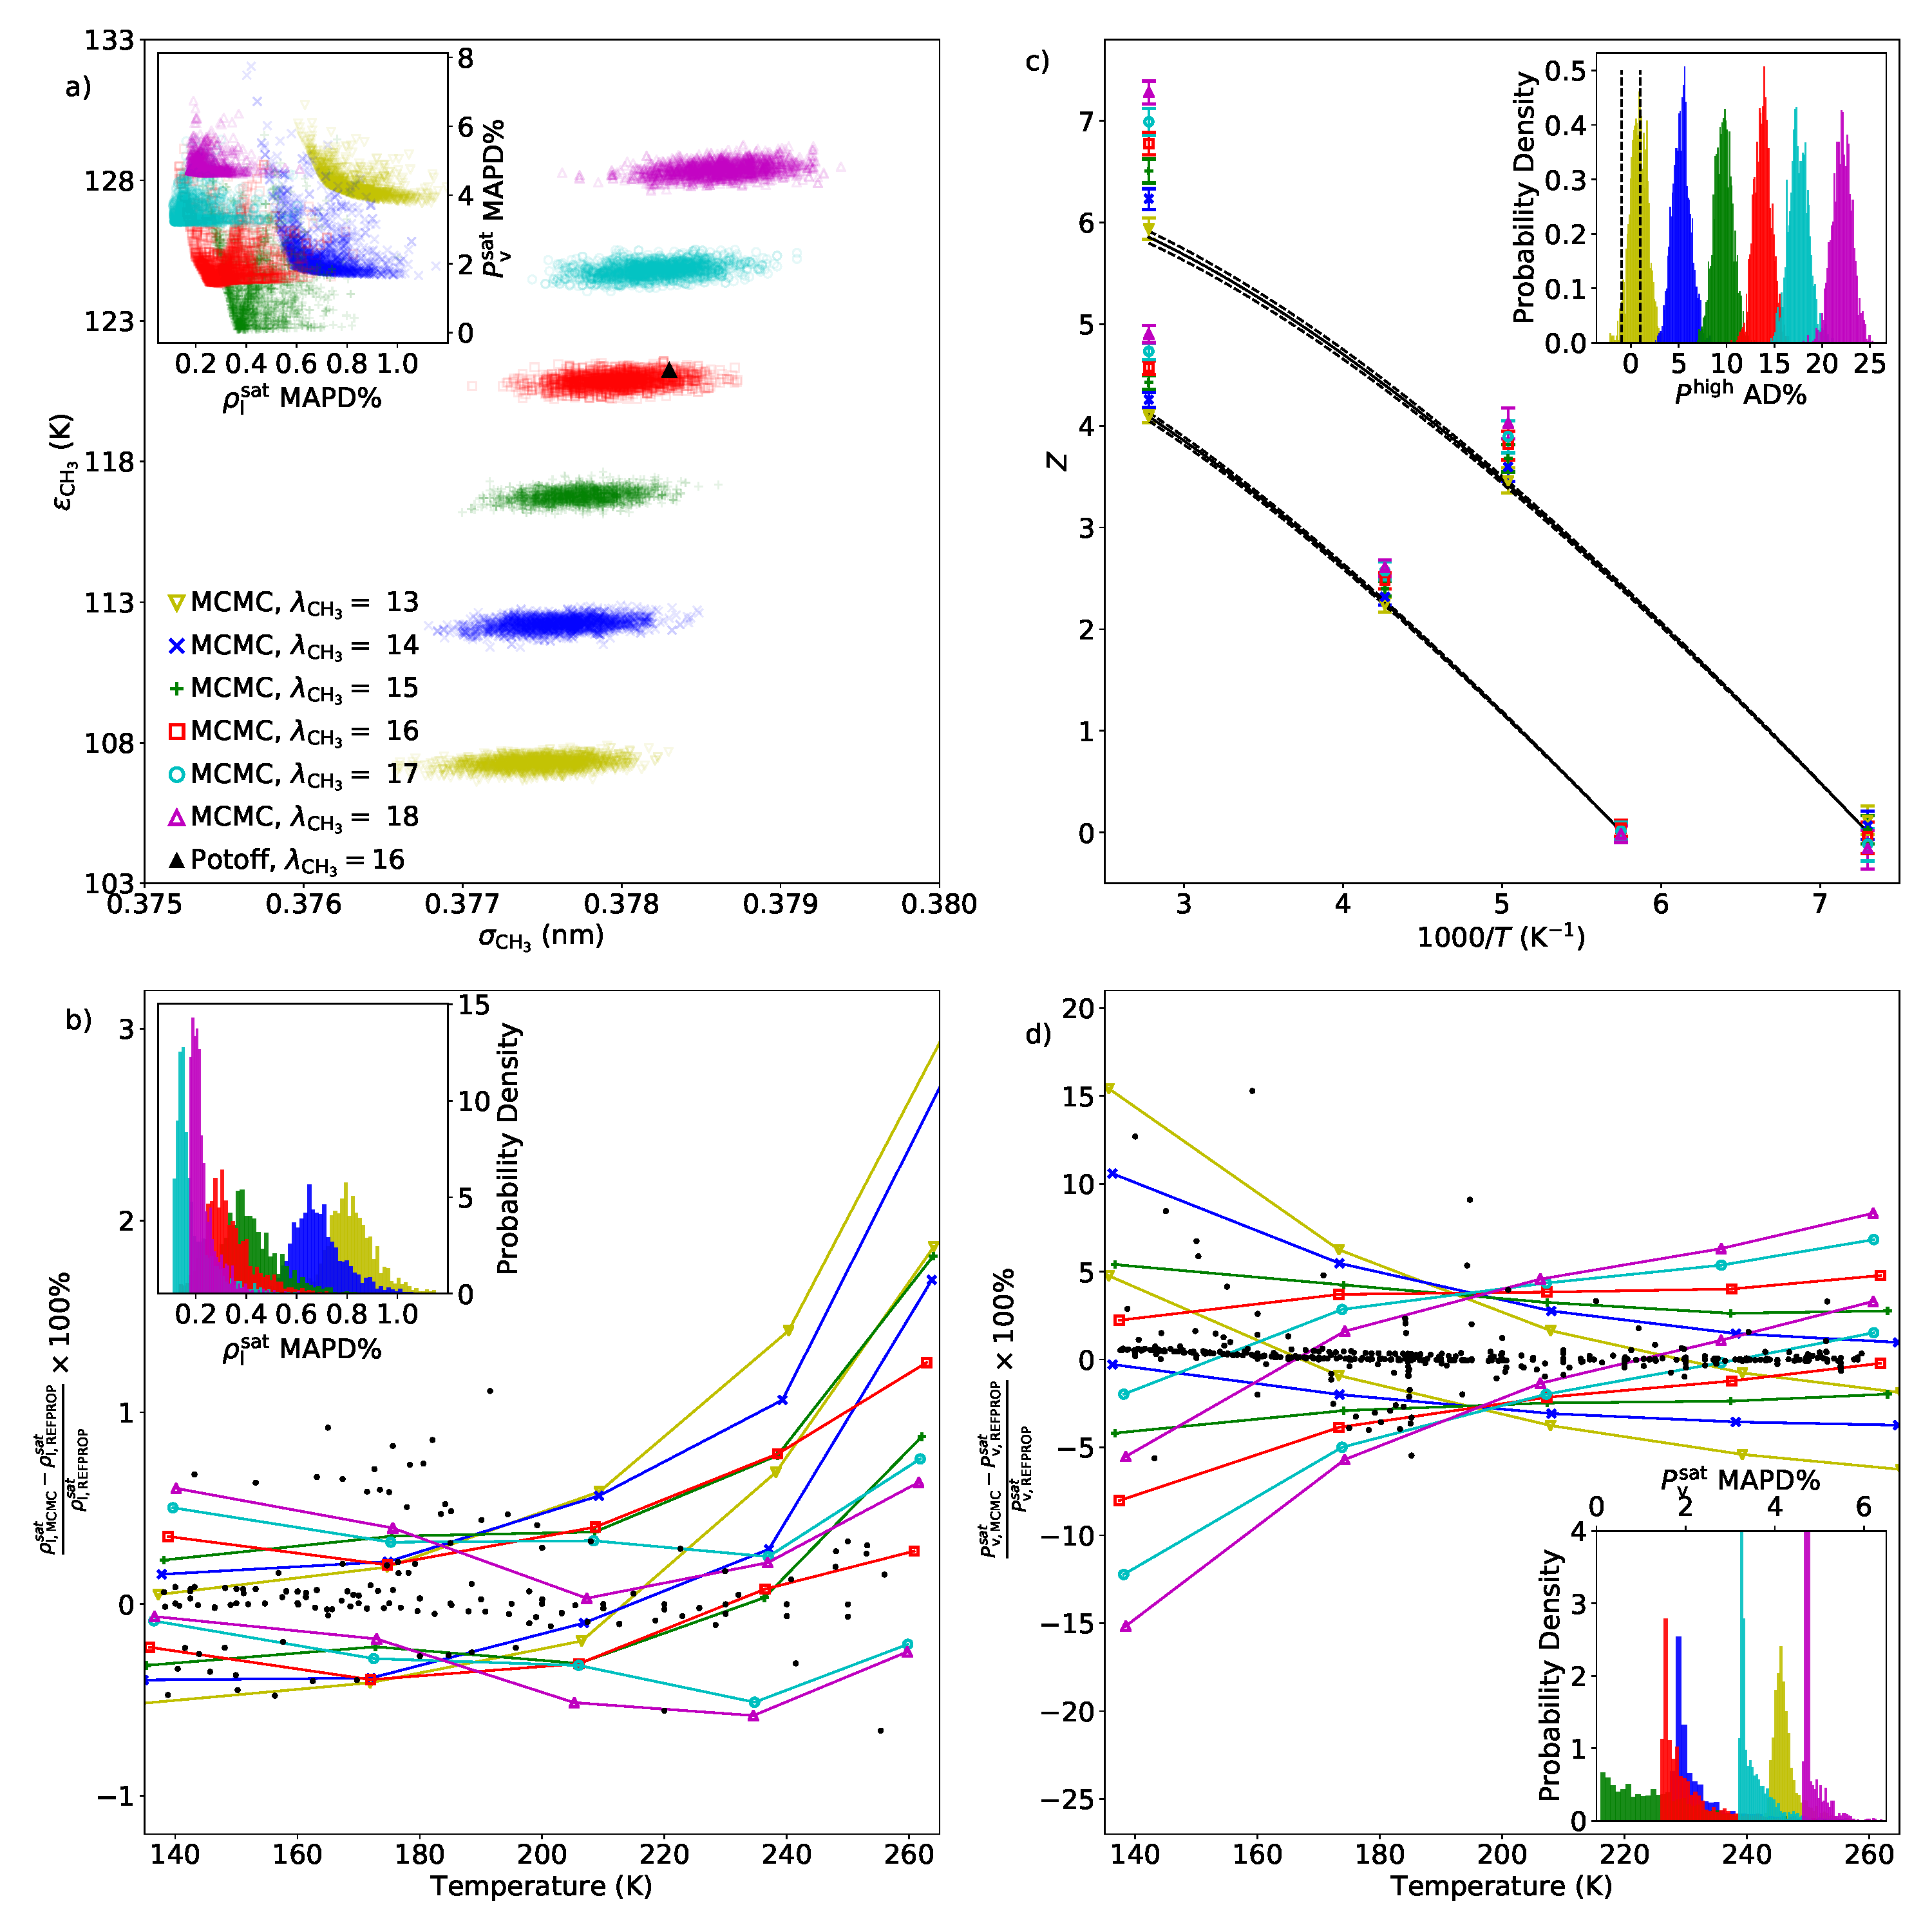
\includegraphics[width=6.4in]{MCMC_Mie_13_14_15_16_17_18_ethane}
%	\caption{MCMC results quantify the uncertainty in $\epsilon_{\rm CH_3}$--$\sigma_{\rm CH_3}$ and how these uncertainties propagate for $\rho_{\rm l}^{\rm sat}$, $P_{\rm v}^{\rm sat}$, and $Z$. Panel a) plots the MCMC sampled parameter sets for different values of $\lambda_{\rm CH_3}$ ($\epsilon_{\rm CH_3, MCMC}$ and $\sigma_{\rm CH_3, MCMC}$) and the Potoff parameter set as a reference.  Panels b) and d) plot the percent deviation from REFPROP correlations for $\rho_{\rm l, MCMC}^{\rm sat}$ and $P_{\rm v, MCMC}^{\rm sat}$, respectively, where the upper and lower lines correspond to the 95\% credible level for each $\lambda$. Insets of Panels b) and d) are histograms of the MAPD\% in $\rho_{\rm l, MCMC}^{\rm sat}$ and $P_{\rm v, MCMC}^{\rm sat}$, respectively. Experimental data used to compute the likelihood are included in Panels b) and d) as black dots. Panel c) plots $Z$ with respect to inverse temperature for the two highest isochore densities $(\rho_3$ and $\rho_4)$. Inset of Panel c) plots the distribution of average deviation (AD\%) in $P^{\rm high}$, i.e. pressure for $\rho_3$--$\rho_4$ and $T = T^{\rm IT}$. REFPROP uncertainty in $P^{\rm high}$ is $\pm 1$\%.}
%	%MRS2: is the spread in exprimental data at each T the experimental uncertainty? I'm not entirely sure only one property is being predicted, meaning the spread is noise in a single obserbable.
%	%RAM2: The experimental data are just included to give a sense for the goodness of fit. Is your point that I should not include them? 
%	\label{fig:MCMC_Mie_13_14_15_16_17_18_ethane}
%\end{figure} 
%
%The results depicted in Figure \ref{fig:MCMC_Mie_13_14_15_16_17_18_ethane} Panels b)-d) are useful for comparing the performance of different values of $\lambda$ for $\rho_{\rm l}^{\rm sat}$, $P_{\rm v}^{\rm sat}$, and $Z$, respectively. Notice that the insets in Panels b) and d) plot the mean absolute percent deviation (MAPD\%) to quantify the goodness of fit to VLE data, while the inset in Panel c) plots the average deviation (AD\%) to demonstrate the positive bias in $P^{\rm high}$. Note that because MAPD\% and AD\% are percent deviations they are not directly related to the posterior distribution since our likelihood is a normal distribution, which is based on squared deviations. However, we plot MAPD\% and AD\% as these are easier to conceptualize and quantify. 
%
%Panel b) with the corresponding inset demonstrates that the best prediction of $\rho_{\rm l}^{\rm sat}$ is obtained for higher values of $\lambda_{\rm CH_3}$. However, while the $\rho_{\rm l}^{\rm sat}$ MAPD\% for $\lambda_{\rm CH_3} = 15$--$18$ are similar, $\lambda_{\rm CH_3} = 13$--$14$ have significantly higher $\rho_{\rm l}^{\rm sat}$ MAPD\%. 
%
%Panel d) demonstrates that $\lambda_{\rm CH_3} = 13$--$14$ and $\lambda_{\rm CH_3} = 17$--$18$ over- and under-predict $P_{\rm v}^{\rm sat}$ at low temperatures, respectively, 
%%MRS2: eyeballing, 14 looks consistent to me.  What quantitive measure can you use for what it means to over or underpredict?
%%RAM2: The MAPD histogram is intended to quantify this statement. Also, I just realized that I had an error in panels b,c, and d. Specifically, the errorbars and uncertainty regions represented the estimated 100% confidence region, i.e. all of the MCMC sampled values. I have now converted these to the 95% credible regions by integrating the histograms with equal areas. The results are much more conclusive now.
%while $\lambda_{\rm CH_3} = 15$--$16$ are the most reliable. $\lambda_{\rm CH_3} = 15$ has the least amount of bias and the lowest MAPD\% in $P_{\rm v}^{\rm sat}$ (see inset). 
%
%Finally, Panel c) demonstrates that all of the sampled $\epsilon_{\rm CH_3, MCMC}$ and $\sigma_{\rm CH_3, MCMC}$ parameter sets for $\lambda_{\rm CH_3} \ge 14$ over-predict $Z$ at high temperatures and densities $(P^{\rm high})$. As expected, the larger the value of $\lambda_{\rm CH_3}$, the 
%more 
%%greater 
%the force field over-predicts $P^{\rm high}$.

Figures \ref{fig:MCMC_ethane_parameter_space}-\ref{fig:MCMC_Mie_13_14_15_16_17_18_ethane_Pareto} present the MCMC results for ethane with $\lambda_{\rm CH_3} =13$-$18$. Figure \ref{fig:MCMC_ethane_parameter_space} demonstrates that the feasible region of $\epsilon_{\rm CH_3}$ depends strongly on $\lambda_{\rm CH_3}$, namely, larger values of $\lambda_{\rm CH_3}$ require larger values of $\epsilon_{\rm CH_3}$. By contrast, we observe a much smaller shift towards larger values of $\sigma_{\rm CH_3}$ with increasing $\lambda_{\rm CH_3}$. This observation is consistent with Reference \citenum{Mie}.
% the literature \cite{Mie}.

\begin{figure}[htb!]
	\centering
	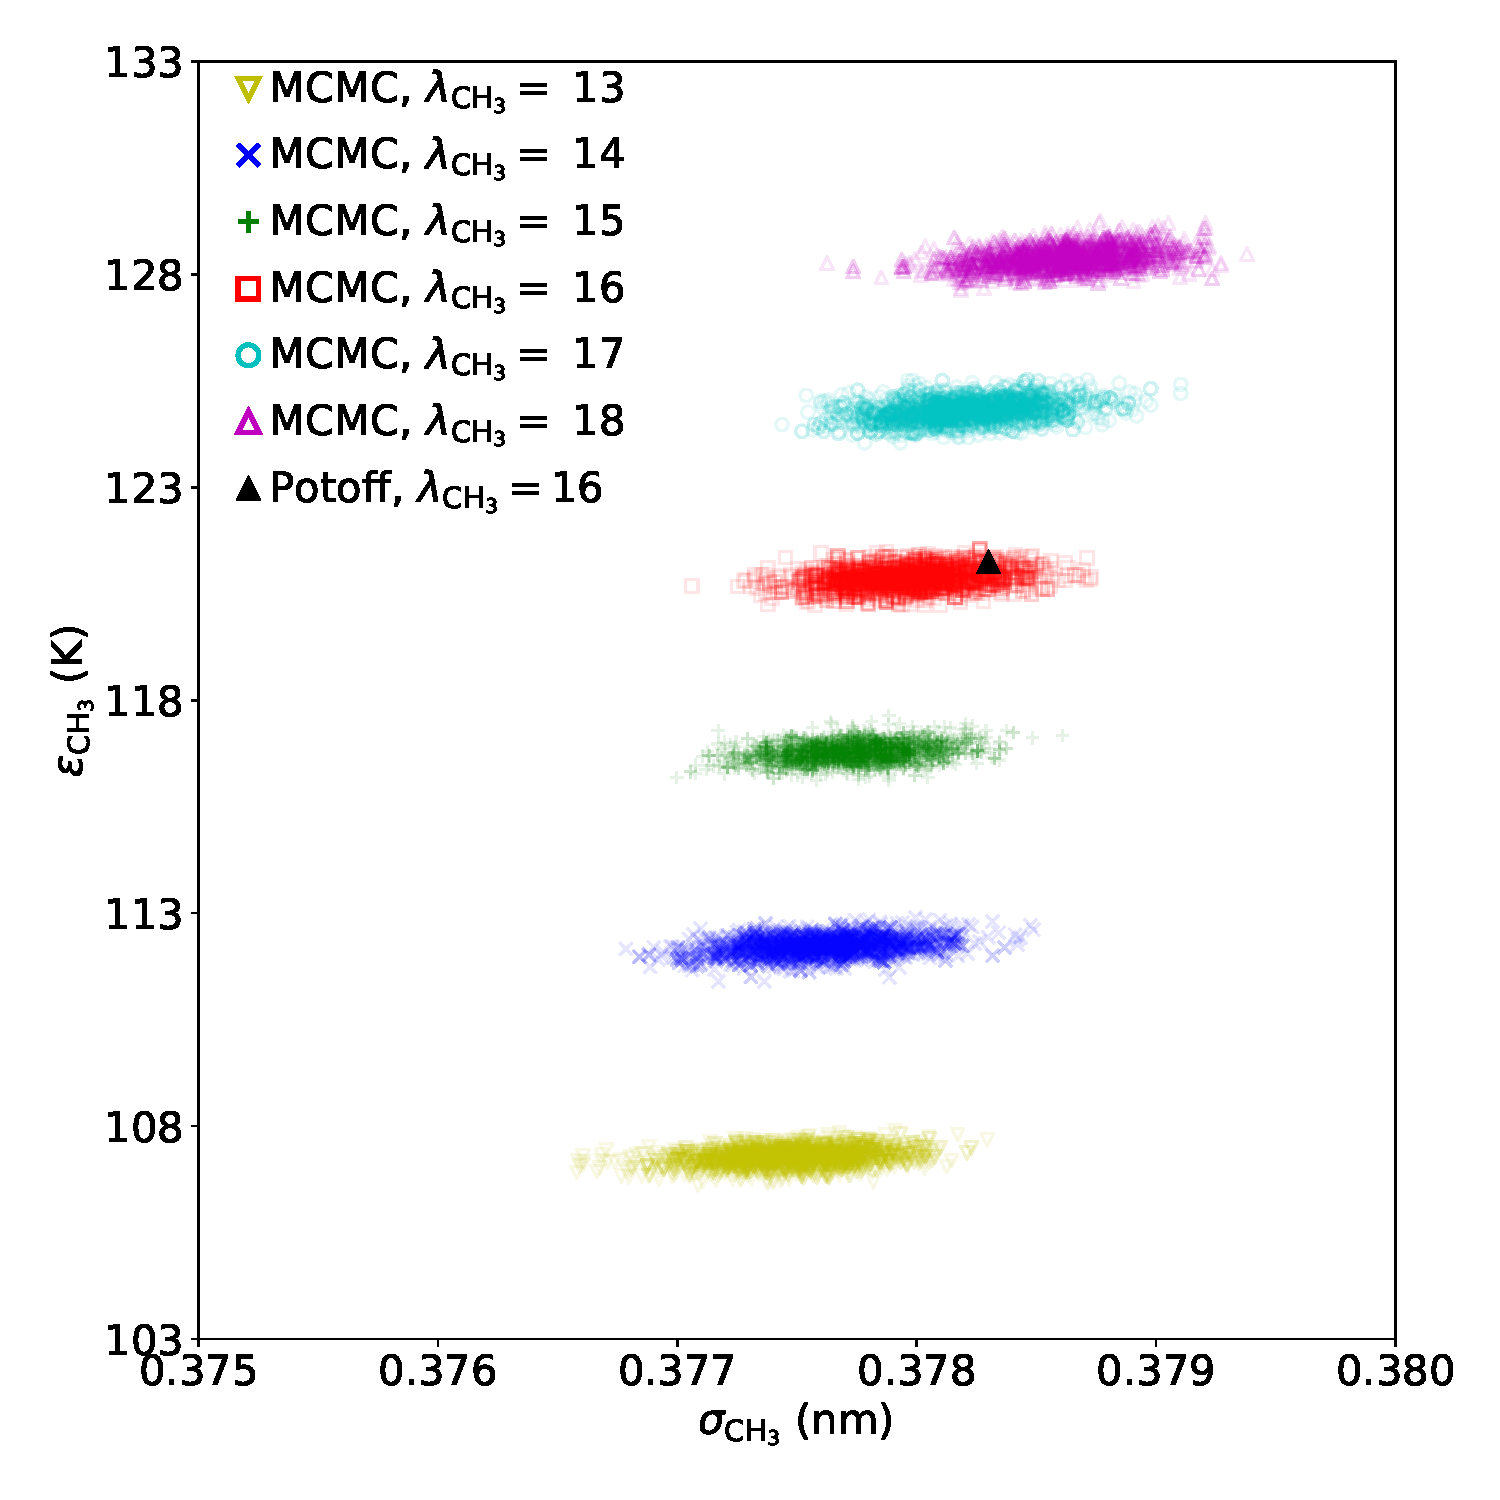
\includegraphics[width=3.2in]{MCMC_ethane_parameter_space}
	\caption{MCMC sampled parameter sets for different values of $\lambda_{\rm CH_3}$ ($\epsilon_{\rm CH_3, MCMC}$ and $\sigma_{\rm CH_3, MCMC}$) quantify the uncertainty in $\epsilon_{\rm CH_3}$--$\sigma_{\rm CH_3}$. The Potoff parameter set is included as a reference for $\lambda_{\rm CH_3} = 16$.} 
	\label{fig:MCMC_ethane_parameter_space}
\end{figure}
%MRS3: are useful isn't a good topic sentence, because it doesn't say what they are useful for.  Better to say what they are useful for.
%RAM3: Done
%The results depicted in 
Figures \ref{fig:MCMC_ethane_VLE}-\ref{fig:MCMC_ethane_Phigh} compare the performance of different values of $\lambda$ for $\rho_{\rm l}^{\rm sat}$, $P_{\rm v}^{\rm sat}$, and $Z$. Notice that the insets in Figure \ref{fig:MCMC_ethane_VLE} plot the mean absolute percent deviation (MAPD\%) to quantify the goodness of fit to VLE data, while the inset in Figure \ref{fig:MCMC_ethane_Phigh} plots the average deviation (AD\%) to demonstrate the positive bias in $P^{\rm high}$. Note also that because MAPD\% and AD\% are percent deviations they are not directly related to the squared deviations of the normal distribution used to compute the likelihood. We plot MAPD\% and AD\% as these are easier to conceptualize and quantify. 

\begin{figure}[htb!]
	\centering
	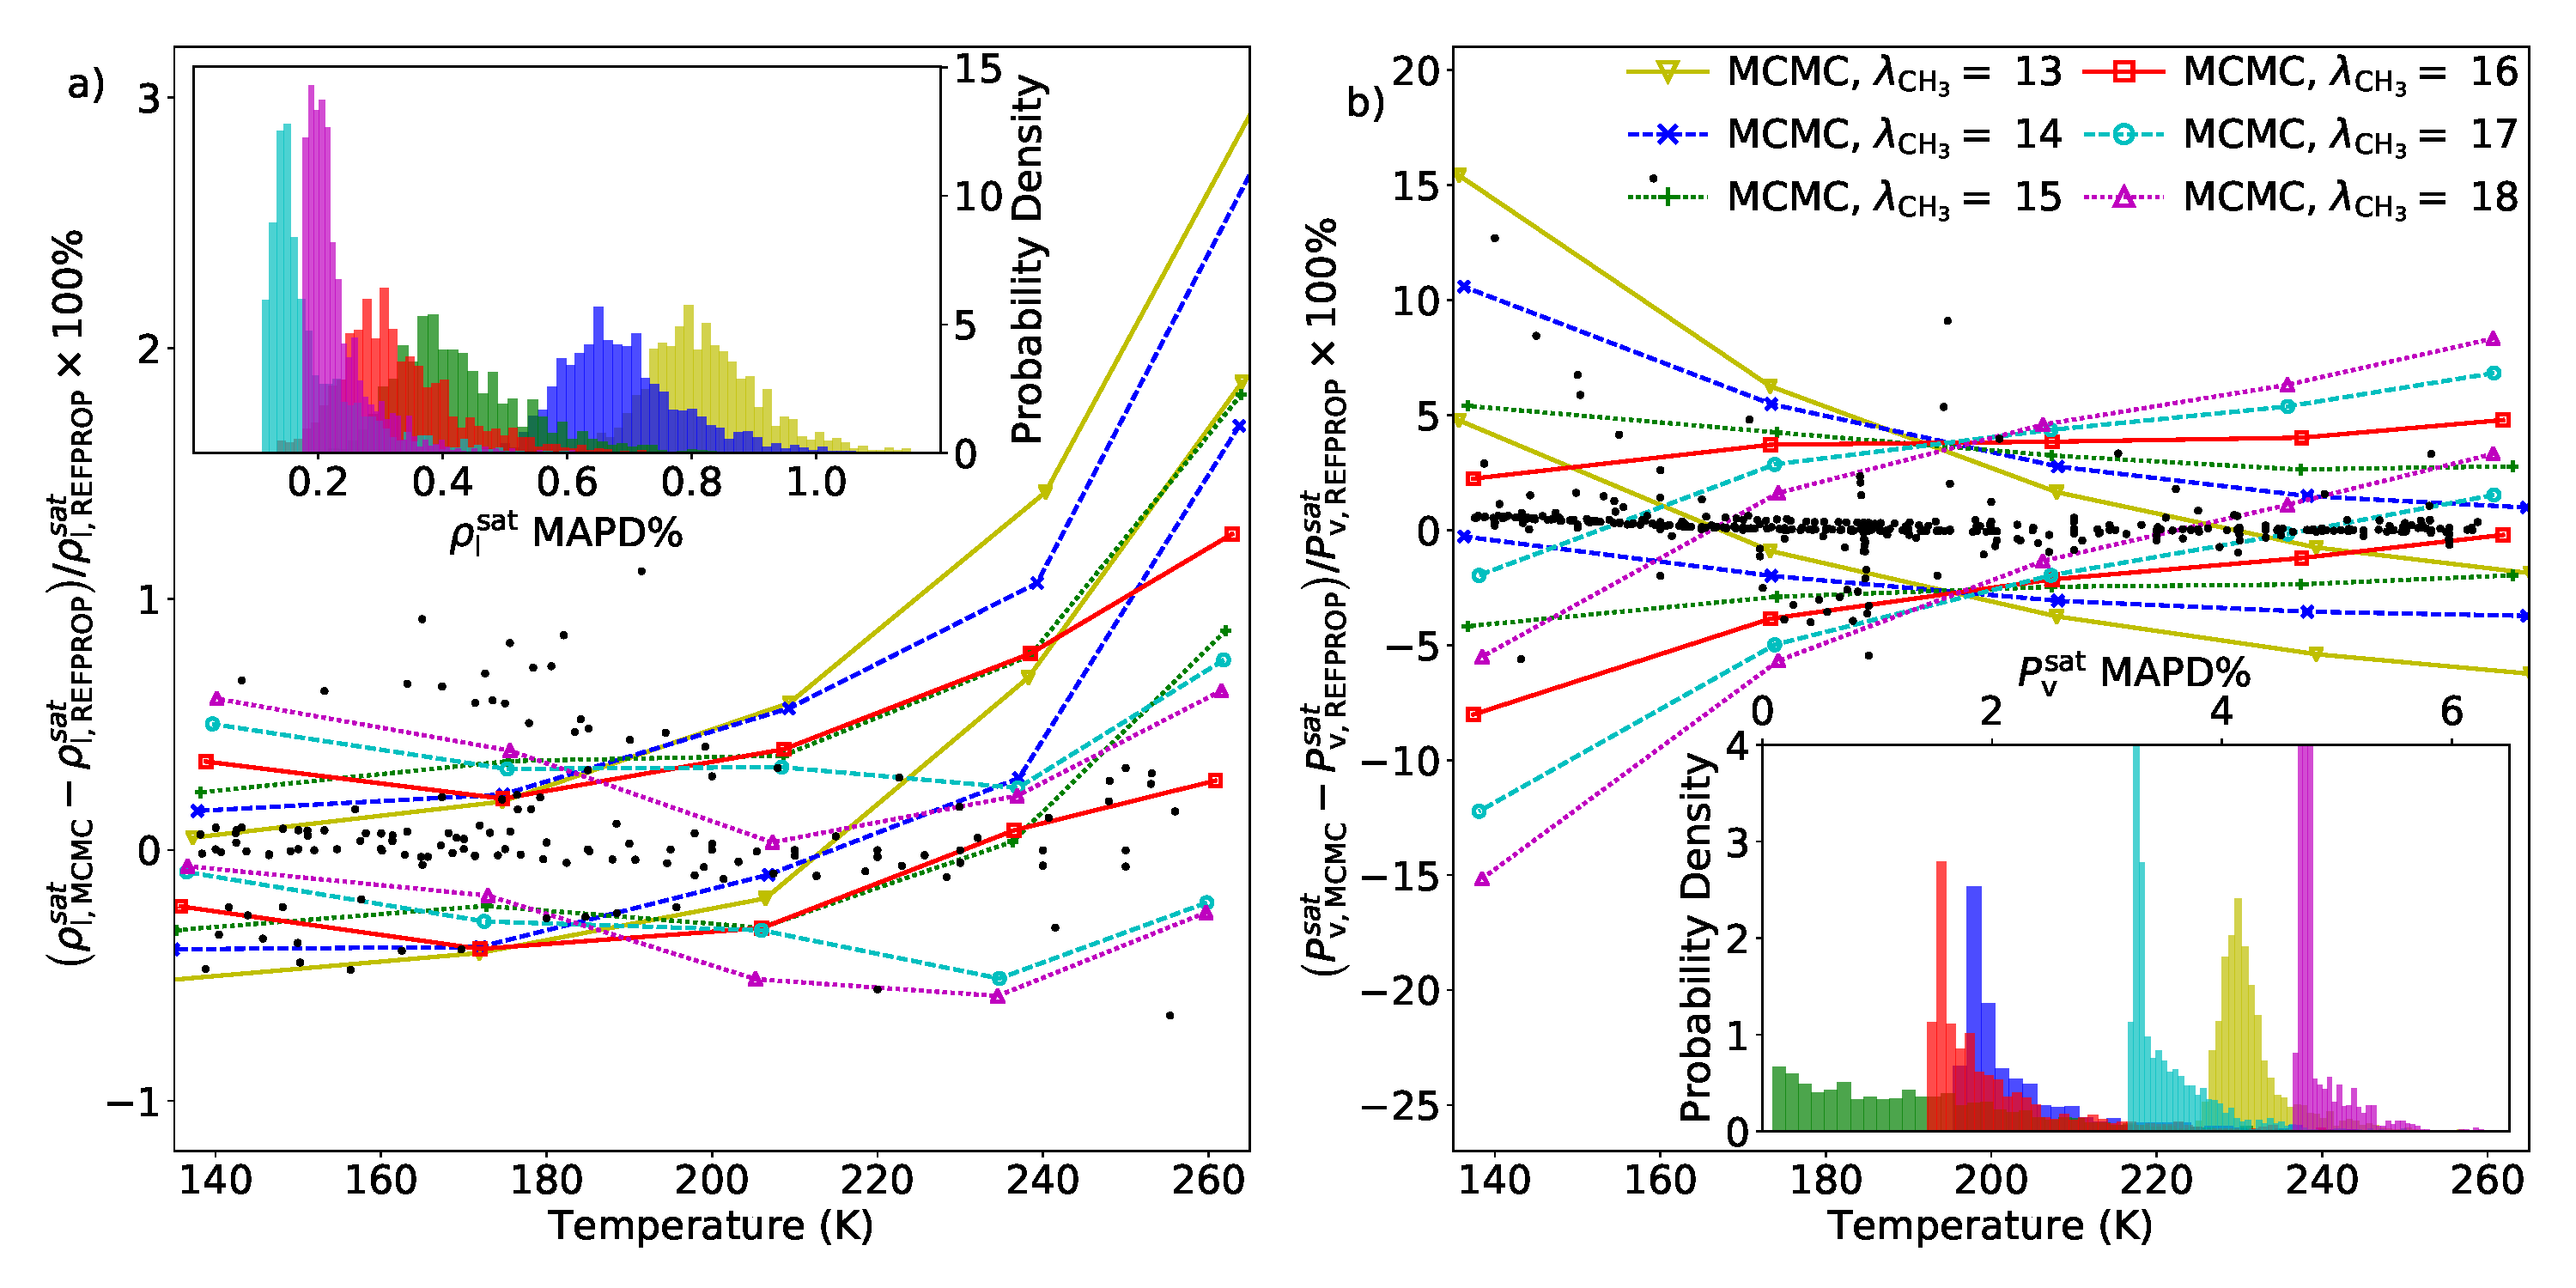
\includegraphics[width=6.4in]{MCMC_ethane_VLE}
%MRS3: this chart is still more confusing that it needs to be.  It's not immediately clear that the colors in the lines are also the colors for the histogram.  Why insets?  why not a 4 part graph? You could make the two histograms smaller by changing the aspect ratio (so just as broad, but not as high). You don't need to put everything in the same small space. It's also more typical if a legend is for two subfigures, to have the legend outside and centered, so it's clearer it belongs to both.  The histograms might benefit from some turning down opacity, so all the colors are clear.  
%MRS3: I'm also not clear that this is a great opening line to the caption. IS the main point of the graph that uncertainties propagate? 
	\caption{Robust posterior prediction propagates $\epsilon_{\rm CH_3}$--$\sigma_{\rm CH_3}$ parameter uncertainties to $\rho_{\rm l}^{\rm sat}$ and $P_{\rm v}^{\rm sat}$. Panels a)--b) plot the percent deviation from REFPROP correlations for $\rho_{\rm l, MCMC}^{\rm sat}$ and $P_{\rm v, MCMC}^{\rm sat}$, respectively. The upper and lower lines for each $\lambda$ correspond to the 95\% credible interval obtained from $QoI_{\rm MCMC}$. Insets of Panels a)--b) are histograms of the MAPD\% in $\rho_{\rm l, MCMC}^{\rm sat}$ and $P_{\rm v, MCMC}^{\rm sat}$, respectively. Experimental data used to compute the likelihood are included as black dots.}
	%MRS2: is the spread in exprimental data at each T the experimental uncertainty? I'm not entirely sure only one property is being predicted, meaning the spread is noise in a single obserbable.
	%RAM2: The experimental data are just included to give a sense for the goodness of fit. Is your point that I should not include them? 
	\label{fig:MCMC_ethane_VLE}
\end{figure}

Figure \ref{fig:MCMC_ethane_VLE} Panel a) with the corresponding inset demonstrates that the best prediction of $\rho_{\rm l}^{\rm sat}$ is obtained for higher values of $\lambda_{\rm CH_3}$. However, while the $\rho_{\rm l}^{\rm sat}$ MAPD\% for $\lambda_{\rm CH_3} = 15$--$18$ are similar, $\lambda_{\rm CH_3} = 13$--$14$ have significantly higher $\rho_{\rm l}^{\rm sat}$ MAPD\%. Figure \ref{fig:MCMC_ethane_VLE} Panel b) demonstrates that $\lambda_{\rm CH_3} = 13$--$14$ and $\lambda_{\rm CH_3} = 17$--$18$ over- and under-predict $P_{\rm v}^{\rm sat}$ at low temperatures, respectively, 
%MRS2: eyeballing, 14 looks consistent to me.  What quantitive measure can you use for what it means to over or underpredict?
%RAM2: The MAPD histogram is intended to quantify this statement. Also, I just realized that I had an error in panels b,c, and d. Specifically, the errorbars and uncertainty regions represented the estimated 100% confidence region, i.e. all of the MCMC sampled values. I have now converted these to the 95% credible regions by integrating the histograms with equal areas. The results are much more conclusive now.
while $\lambda_{\rm CH_3} = 15$--$16$ have the best trend for $P_{\rm v}^{\rm sat}$. The inset for Panel b) shows that $\lambda_{\rm CH_3} = 15$ has the lowest MAPD\% in $P_{\rm v}^{\rm sat}$.
% are the most reliable. $\lambda_{\rm CH_3} = 15$ has the least amount of bias and the lowest MAPD\% in $P_{\rm v}^{\rm sat}$ (see inset). 

\begin{figure}[htb!]
	\centering
	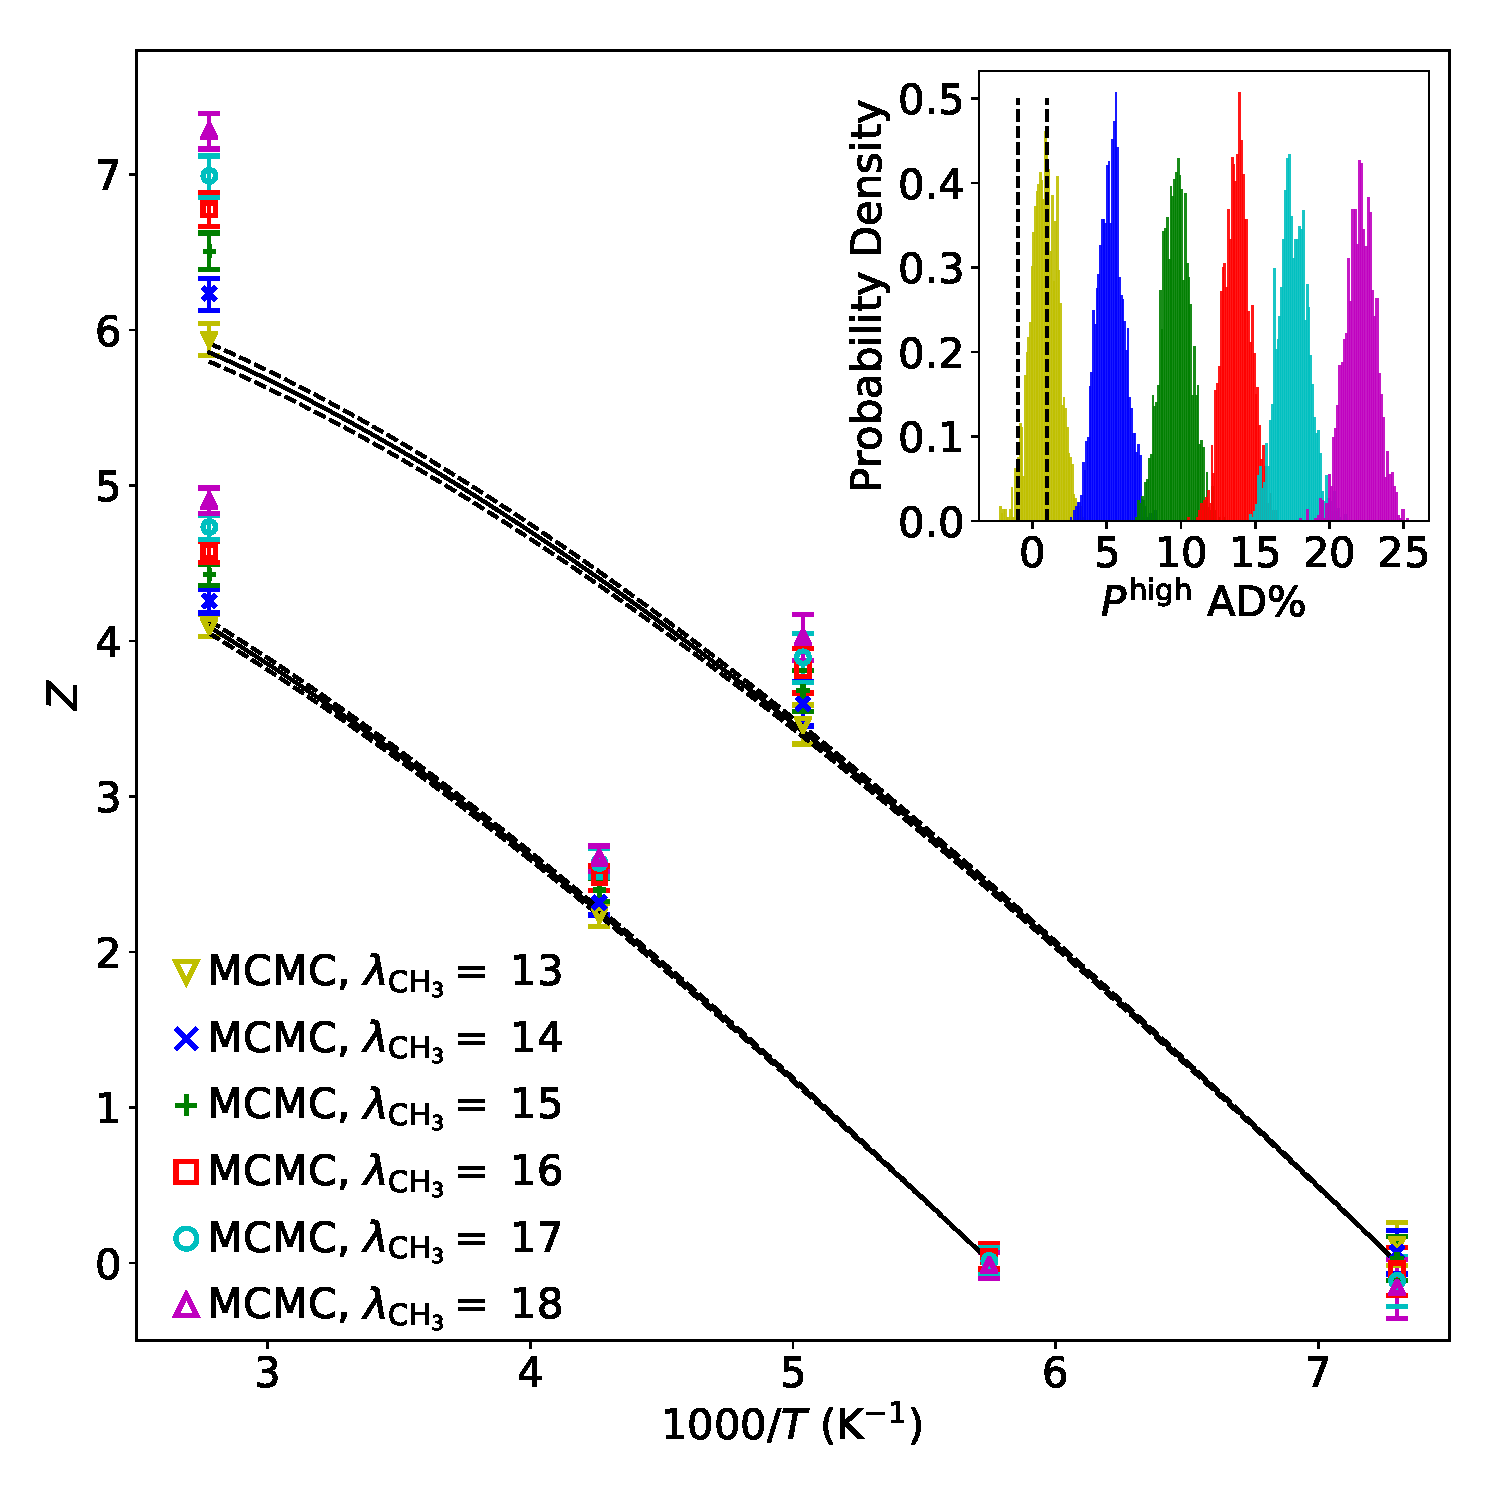
\includegraphics[width=3.2in]{MCMC_ethane_Phigh}
	\caption{Inadequacies of the UA Mie $\lambda$-6 potential are observed in $Z$ for the two highest isochore densities $(\rho_3$ and $\rho_4)$ by propagating the uncertainties in $\epsilon_{\rm CH_3}$--$\sigma_{\rm CH_3}$ for different values of $\lambda_{\rm CH_3}$. The inset plots the distribution of average deviation (AD\%) in $P^{\rm high}$, i.e. $P_{\rm MCMC}$ for $\rho = \rho_3$--$\rho_4$ and $T = T^{\rm IT}$. REFPROP uncertainty in $P^{\rm high}$ is $\pm 1$\%.}
	\label{fig:MCMC_ethane_Phigh}
\end{figure} 

Finally, Figure \ref{fig:MCMC_ethane_Phigh} demonstrates that all of the sampled $\epsilon_{\rm CH_3, MCMC}$ and $\sigma_{\rm CH_3, MCMC}$ parameter sets for $\lambda_{\rm CH_3} \ge 14$ over-predict $Z$ at high temperatures and densities $(P^{\rm high})$. As expected, the larger the value of $\lambda_{\rm CH_3}$, the 
more 
%greater 
the force field over-predicts $P^{\rm high}$.

While Figures \ref{fig:MCMC_ethane_VLE}-\ref{fig:MCMC_ethane_Phigh} plot the results for $\rho_{\rm l}^{\rm sat}$, $P_{\rm v}^{\rm sat}$, and $Z$ individually, Figure \ref{fig:MCMC_Mie_13_14_15_16_17_18_ethane_Pareto} helps to visualize the overall performance of different values of $\lambda_{\rm CH_3}$ for simultaneously predicting all three quantities of interest. 
%MRS2: be more precise about noticing the pareto front.  You mean in Panel a?) Can you draw a line indicating it? Some people might not have a sense of what they would be looking for.
In Panel a), notice the trade-off between the MAPD\% of $\rho_{\rm l}^{\rm sat}$ and $P_{\rm v}^{\rm sat}$. This compromise between two competing properties included in the objective function, namely, $\rho_{\rm l}^{\rm sat}$ and $P_{\rm v}^{\rm sat}$, is known as a Pareto front \cite{Pareto_Deriv,Pareto_LJPQ,Pareto_ST}. The optimal location for a Pareto front is the bottom left region of the plot (low MAPD\% for both $\rho_{\rm l}^{\rm sat}$ and $P_{\rm v}^{\rm sat}$) while the worst location is the top right region (high MAPD\% for both $\rho_{\rm l}^{\rm sat}$ and $P_{\rm v}^{\rm sat}$). Note that the inset of Panel a) includes an approximate ``overall'' Pareto front that combines the results for all values of $\lambda_{\rm CH_3}$. Although not depicted for visual clarity, the ``L'' shaped frontier for different colors/symbols demonstrates that each $\lambda_{\rm CH_3}$ value also has its own Pareto front. Because the overall Pareto front consists of points from the $\lambda_{\rm CH_3} = 15$--$17$ Pareto fronts, the Pareto optimal $\lambda_{\rm CH_3}$ value is either $15$, $16$, or $17$, depending on the relative weight assigned to $\rho_{\rm l}^{\rm sat}$ and $P_{\rm v}^{\rm sat}$. By contrast, since the $\lambda_{\rm CH_3} = 13$, $14$, and $18$ Pareto fronts are completely inside the overall Pareto front, these $\lambda_{\rm CH_3}$ values are not optimal, regardless of the weighting.

\begin{figure}[p!]
	\centering
	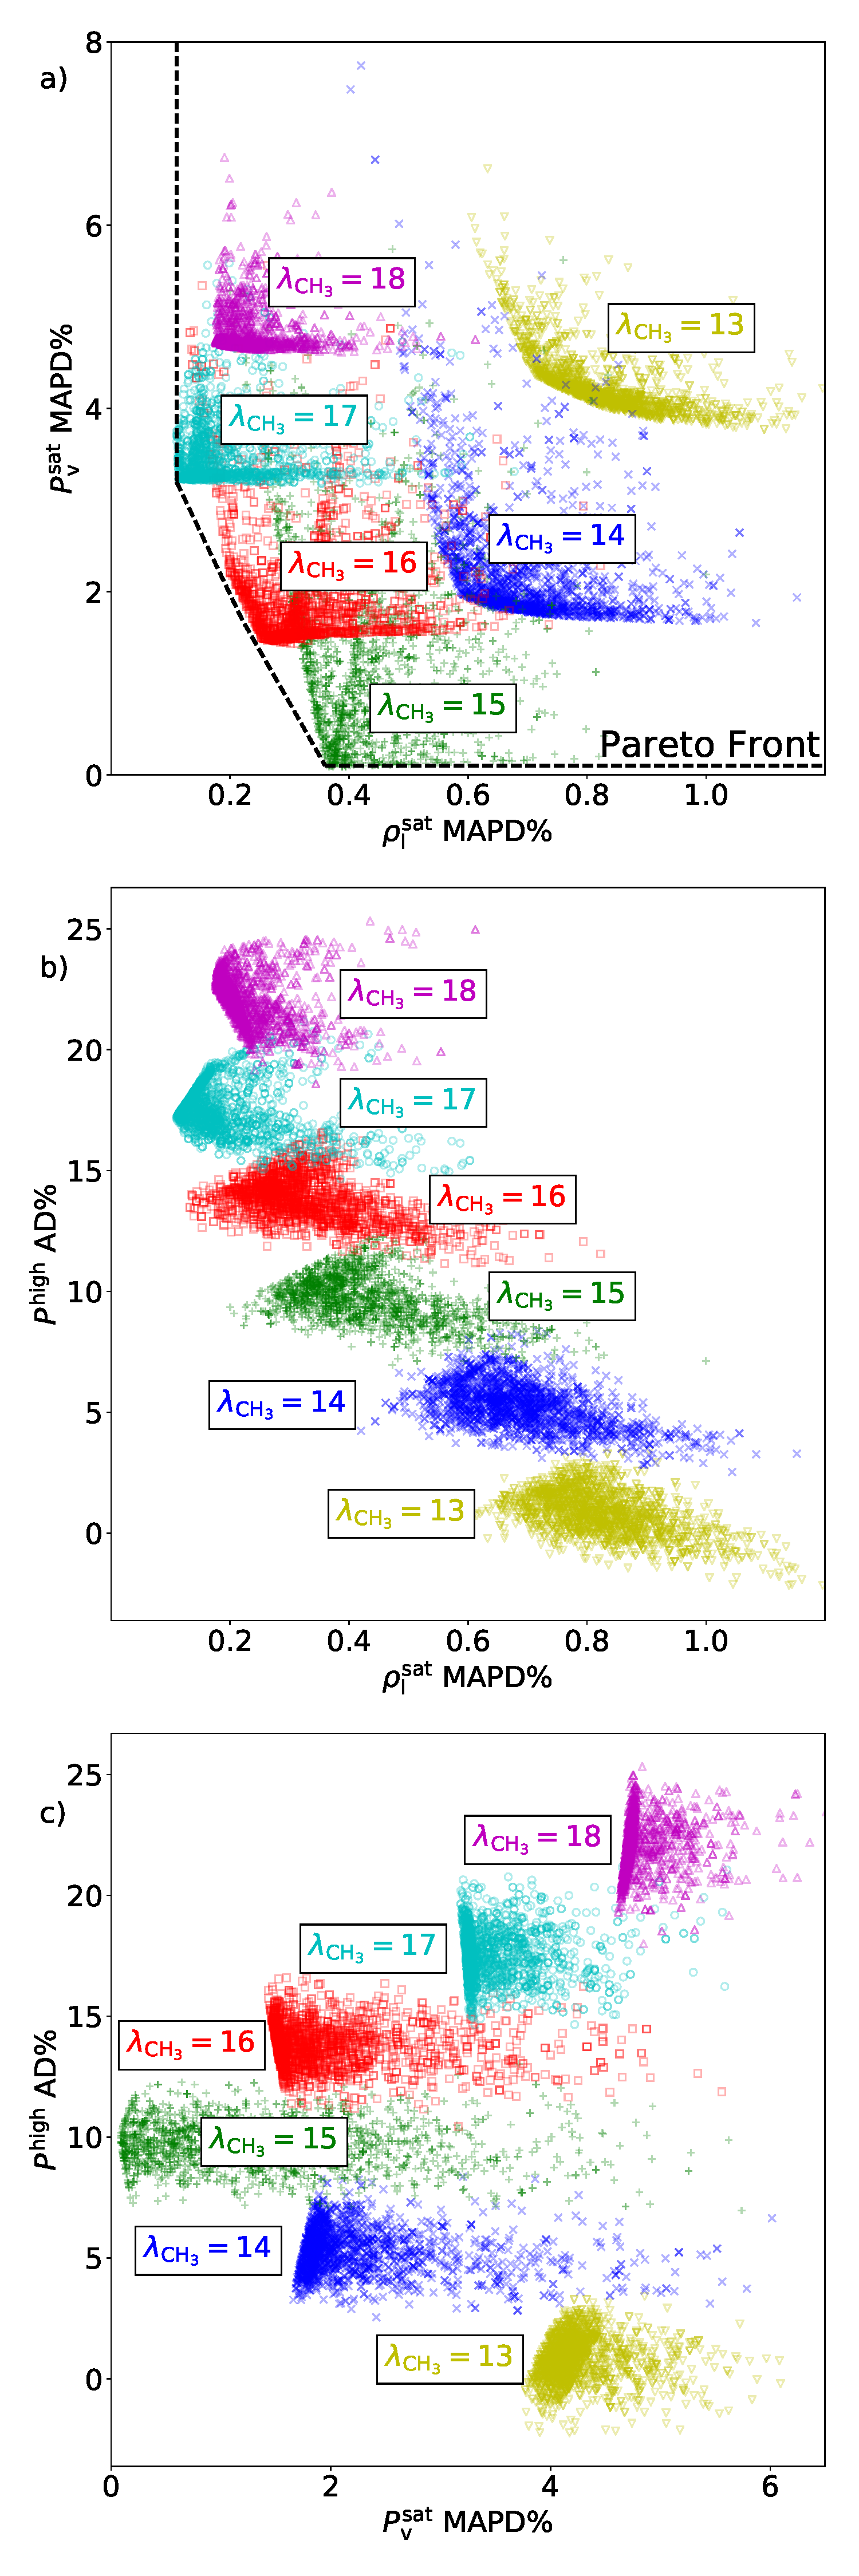
\includegraphics[width=2.5in]{MCMC_Mie_13_14_15_16_17_18_ethane_Pareto}
%MRS3: maybe a bit more specific a figure caption first sentence?  In what way do they show that?  Pareto fronts show that?
	\caption{MCMC results confirm that the UA Mie $\lambda$-6 potential cannot adequately predict both VLE and high pressures for supercritical fluids and compressed liquids. Panel a) plots the mean absolute percent deviation (MAPD\%) of $\rho_{\rm l, MCMC}^{\rm sat}$ and $P_{\rm v, MCMC}^{\rm sat}$. Panels b)-c) plot the average deviation (AD\%) in $P^{\rm high}$ with respect to MAPD\% of $\rho_{\rm l, MCMC}^{\rm sat}$ and $P_{\rm v, MCMC}^{\rm sat}$, respectively.}
	\label{fig:MCMC_Mie_13_14_15_16_17_18_ethane_Pareto}
\end{figure} 


Finally, and most importantly for our purposes, Figure \ref{fig:MCMC_Mie_13_14_15_16_17_18_ethane_Pareto} Panels b)-c) demonstrate the 
%MRS3: is depreciation the right word? Lowering in value? 
%RAM3: Reworded
increase in MAPD\% for $\rho_{\rm l}^{\rm sat}$ and $P_{\rm v}^{\rm sat}$ that accompanies more accurate prediction of $P^{\rm high}$. For example, although $\lambda_{\rm CH_3} = 15$, $16$, and $17$ are the best values based on VLE data, they over-predict $P^{\rm high}$ by around 10, 14, and 18\%, respectively. By contrast, while $\lambda_{\rm CH_3} = 13$ is the most accurate for $P^{\rm high}$, the MAPD\% for $\rho_{\rm l}^{\rm sat}$ and $P_{\rm v}^{\rm sat}$ are $4$ and $40$ factors larger than the respective minimum MAPD\%. These results support the fundamental claim of this work, namely, that the UA Mie $\lambda$-6 potential cannot adequately predict both VLE and high pressures for supercritical fluids and compressed liquids. 

%MRS:
%To statistically verify this statement, 
Figure \ref{fig:Bayes_Factors} shows that UA Mie $\lambda$-6 potentials cannot predict both VLE and high pressure properties by comparing the Bayes factor for each value of $\lambda_{\rm CH_3}$ (normalized with respect to $\lambda_{\rm CH_3} = 14$) based solely on $\rho_{\rm l}^{\rm sat}$ and $P_{\rm v}^{\rm sat}$. Bayes factors between $1$--$3.2$, $3.2$--$10$, $10$--$32$, $32$--$100$, and $>100$ are typically classified as ``not substantial'', ``substantial'', ``strong'', ``very strong'', and ``decisive'' evidence, respectively \cite{Jeffreys2004}. With $\frac{3.6}{0.02} = 180$, there is ``decisive'' evidence against the use of $\lambda_{\rm CH_3} = 13$ for predicting $\rho_{\rm l}^{\rm sat}$ and $P_{\rm v}^{\rm sat}$. As $\lambda_{\rm CH_3} = 13$ is the only value that predicts $P^{\rm high}$ within the REFPROP uncertainty, we conclude that no set of $\epsilon_{\rm CH_3}$, $\sigma_{\rm CH_3}$, and $\lambda_{\rm CH_3}$ can predict \textit{both} VLE and $P^{\rm high}$. 

%we compute the Bayes factor for $\lambda_{\rm CH_3} = 13$ based on VLE data. to demonstrate that the evidence for  to quantify evidence for different values of $\lambda_{\rm CH_3}$ .

%While it is clear that $\lambda_{\rm CH_3} = 13$ is optimal for predicting $P^{\rm high}$ Bayes factors quantify the evidence
%
%Although it is clear that the improved accuracy for $P^{\rm high}$ with $\lambda_{\rm CH_3} = 13$  is quite reliable for   
%
%While $\lambda_{\rm CH_3} = 13$ is quite reliable for $P^{\rm high}$, it performs significantly worse for VLE. The Bayes factor, based on VLE data, quantifies the evidence for different values of $\lambda_{\rm CH_3}$. Figure \ref{fig:Bayes_Factors} shows that for ethane the UA Mie 15-6 and 16-6 potentials are equally justified while the evidence for 14-6 and 17-6 is much less and the evidence for 13-6 and 18-6 is negligible. 

%Note that the values in Figure \ref{fig:Bayes_Factors} have been normalized by the 14-6 potential.

% The same is true for the 14-6 potential, which has a 5 AD\% in $P^{\rm high}$  
%While the 14-6 potential only demonstrates a 5\% disagreement in $P^{\rm high}$ (notice that the REFPROP deviation is only 1\%), the deprecation in the quality of VLE is significant. This can be quantified by determining the Bayes factor for different values of $\lambda_{\rm CH_3}$ (normalized by the 14-6 potential). Table \ref{tab:Bayes_Factors} shows that for ethane the 15-6 and 16-6 potentials are equally justified while the evidence for 14-6 and 17-6 is much less and the evidence for 18-6 is negligible.

% the UA Mie 15-6 and 16-6 potentials for ethane (CH$_3$) almost equally, while evidence in Panel b) strongly supports $\lambda_{\rm CH_2} = 16$ over $\lambda_{\rm CH_2} = 14$ for propane and \textit{n}-butane.

\begin{figure}[htb!]
	\centering
	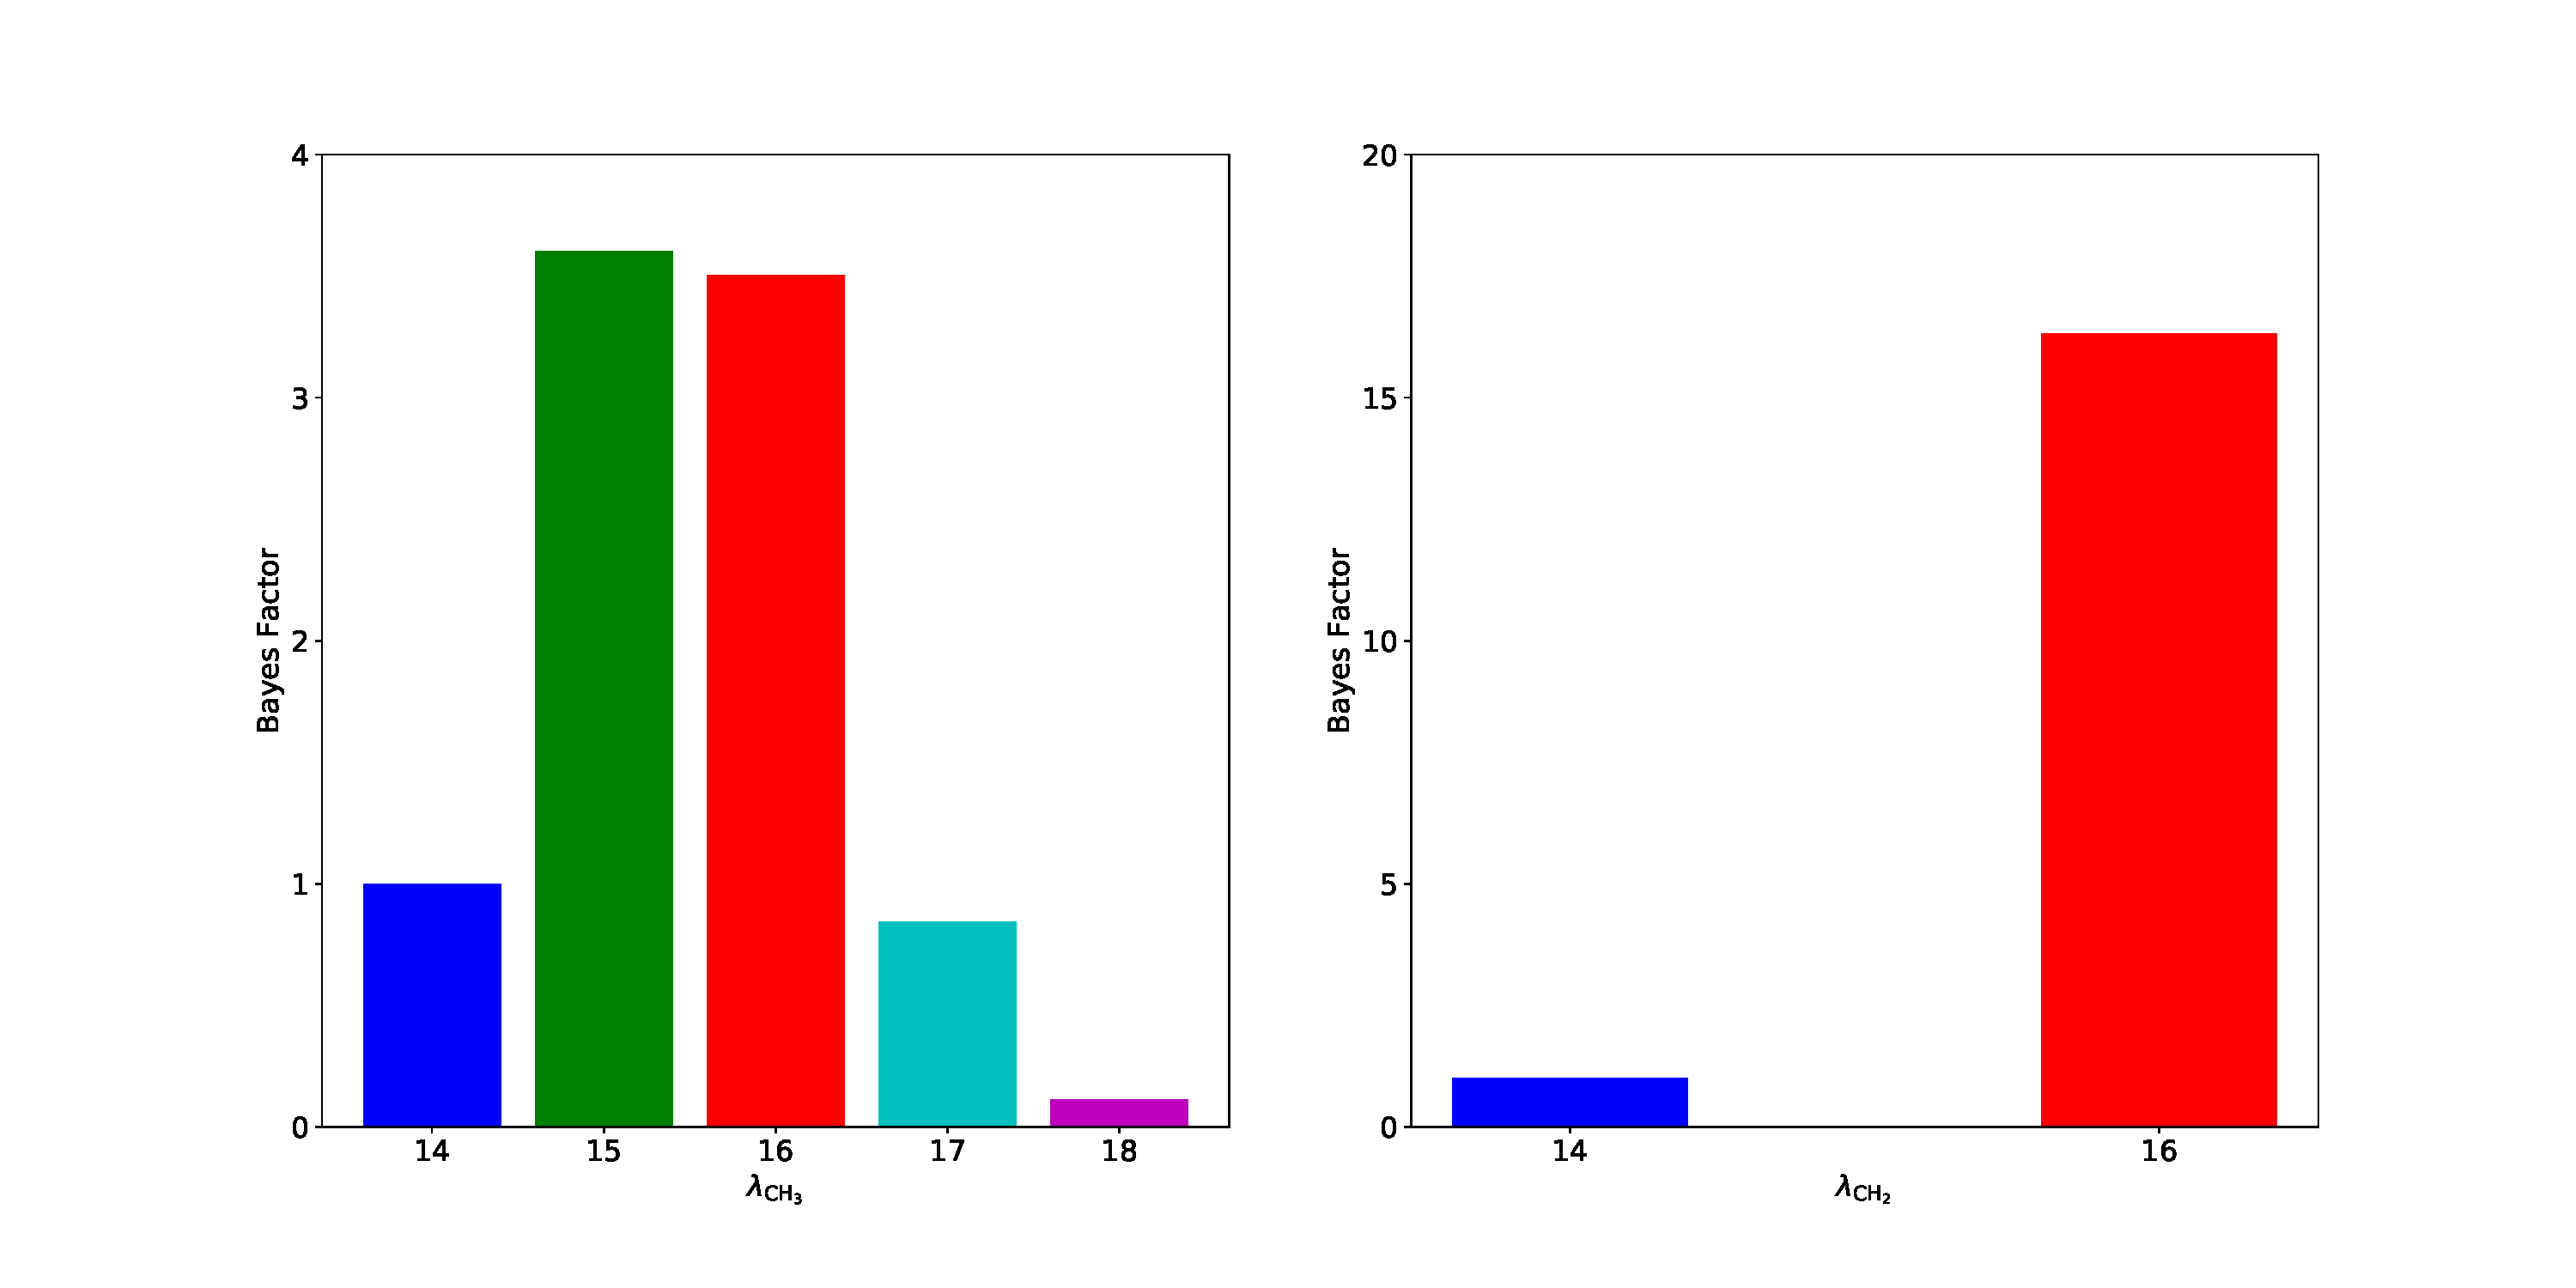
\includegraphics[width=4.8in]{Evidence_Mie_CH3_CH2}
	\caption{Evidence (Bayes factor) in Panel a) supports $\lambda_{\rm CH_3} =15 $ or $16$, while evidence in Panel b) strongly supports $\lambda_{\rm CH_2} = 16$ over $\lambda_{\rm CH_2} = 14$. CH$_3$ values depend only on ethane while CH$_2$ values are based on propane, \textit{n}-butane, and \textit{n}-octane. Note that all values are normalized with respect to $\lambda = 14$.}
	\label{fig:Bayes_Factors}
\end{figure}

%MRS2: I would suggest using a bar chart, not a table (Can put table in supporting).
%RAM2: I orginally had a figure, but I thought it might be overkill. I guess no one really cares about the exact Bayes factors. So maybe a figure would be nice.
%\begin{table}[h!]
%	\caption{Bayes factors for different values of $\lambda$ (normalized by $\lambda= 14$). CH$_3$ values depend on ethane while CH$_2$ values are based on propane and \textit{n}-butane.} \label{tab:Bayes_Factors}
%	\begin{center}
%		\begin{tabular}{|c|c|c|}
%			\hline
%			$\lambda$ & CH$_3$ & CH$_2$ \\ \hline
%			13 & 0.024 & - \\
%			14 & 1. & 1. \\ 
%			15 & 3.6 & - \\  
%			16 & 3.5 & 15.8 \\ 
%			17 & 0.84 & - \\ 
%			18 & 0.11 & - \\  
%			\hline
%		\end{tabular}
%	\end{center} 
%\end{table}

%From Table \ref{tab:Bayes_Factors} it is clear that the 13-6 potential is not justified based on VLE data. The Bayes factor for the 14-6 potential is less conclusive

%The results in Table \ref{tab:Bayes_Factors} are conclusive for the 13-6 potential, a Bayes factor around 
%Although the Bayes factor for the 13-6 potential is conclusive, the 14-6 ,
%
%Although the Bayes factor in Table \ref{tab:Bayes_Factors} is conclusive for the 13-6 potential,

%MRS2: generally, dashes expressing a number range should be --, not -.
%RAM2: Done
%The Bayes factors in Figure \ref{fig:Bayes_Factors} (normalized with respect to $\lambda_{\rm CH_3} = 14$) provide ``very strong'' evidence that the 13-6 and 18-6 potentials are not justified based on ethane VLE data. By contrast, the evidence in favor of the 15-6 and 16-6 potentials over the 14-6 and 17-6 potentials is not as definitive, although a Bayes factor between $3.2$--$10$ is typically considered ``substantial'' (but not ``strong'') evidence \cite{Jeffreys2004}. However, these values depend primarily on the VLE data and the $s^2{\rm D,SM}$ model used to compute $L(\theta|D)$. We use a very conservative error model for $\rho_{\rm l}^{\rm sat}$ and $P_{\rm v}^{\rm sat}$ (see Figure \ref{fig:Error_model}) so that our MCMC samples cover a large region of parameter space. This is done primarily to demonstrate that the UA Mie $\lambda$-6 is inadequate for predicting VLE and $P^{\rm high}$. However, a less conservative error model would provide more convincing evidence regarding the optimal $\lambda$ value based solely on VLE data. 

%The Bayes factors in Figure \ref{fig:Bayes_Factors} (normalized with respect to $\lambda_{\rm CH_3} = 14$) provide evidence for each value of $\lambda_{\rm CH_3}$ based on ethane VLE data. 

In addition, there is ``very strong'' evidence that the 18-6 potential is not justified by VLE data $\left(\frac{3.6}{0.1} = 36\right)$. The evidence in favor of the 15-6 or 16-6 potentials over the 14-6 and 17-6 potentials is not as definitive, although it is still considered ``substantial'' $\left(\frac{3.6 \text{ or } 3.5}{1.0 \text{ or } 0.8} > 3.5\right)$. By contrast, the evidence for $\lambda_{\rm CH_3} = 15$ instead of $\lambda_{\rm CH_3} = 16$ is ``not substantial'' $\left(\frac{3.6}{3.5} \approx 1.03\right)$.

It is important to mention that these Bayes factors depend primarily on the VLE data and the $s^2_{\rm D,SM}$ model used to compute $L(\theta|D)$. We use a very conservative error model for $\rho_{\rm l}^{\rm sat}$ and $P_{\rm v}^{\rm sat}$ (see Figure \ref{fig:Error_model}) so that our MCMC samples cover a large region of parameter space. This is done primarily to demonstrate that the UA Mie $\lambda$-6 is inadequate for predicting VLE and $P^{\rm high}$. However, a less conservative error model would provide more convincing evidence regarding the optimal $\lambda$ value based solely on VLE data. 

Also, ITIC is limited to $T^{\rm sat} < 0.85 T_{\rm c}$. Therefore, it is possible that the optimal value of $\lambda_{\rm CH_3}$ could be deduced (i.e. larger Bayes factors) if higher temperature VLE data were included (say from 260--290 K). Based on the observed bias in $\rho_{\rm l}^{\rm sat}$ at higher temperatures (240--260 K) for $\lambda_{\rm CH_3} = 14$, it appears that higher temperature VLE data would strengthen the counter evidence against the 14-6 potential. It is unclear whether higher temperature data would support the 15-6 or 16-6 potential, although the optimal $\lambda_{\rm CH_3}$ is likely a non-integer value between 15 and 16. 
%MRS2: could just say, some other method such as GCMC may be necessary to access the VLE range of $0.85 T_{\rm c} < T^{\rm sat} < 0.95 T_{\rm c}$.  Don't need to describe future work.
%RAM2: Done
Implementing MBAR with GCMC may be necessary to include VLE data from $0.85 < T_{\rm r}^{\rm sat} < 0.95$.
%, we are working on implementing MBAR with GCMC. 

%While a Bayes factor around 4 is typically not considered substantial evidence, these values depend strongly on the VLE data and the error model used to compute $L(\theta|D)$. We have chosen a very conservative error model to demonstrate the inadequacy in predicting $P^{\rm high}$ (see Section \ref{Surrogate Model}). However, a less conservative error model would provide more convincing evidence for the $\lambda$ Bayes factors. Also, recall that ITIC is limited to $T^{\rm sat} < 0.85 T_{\rm c}$. Therefore, it is possible that the optimal value of $\lambda_{\rm CH_3}$ could be deduced (i.e. larger Bayes factors) if higher temperature VLE data were included (say from 260-290 K). Based on the observed bias in $\rho_{\rm l}^{\rm sat}$ at higher temperatures (240-260 K) for the 14-6 potential, it appears that higher temperature data would strengthen the evidence that the 14-6 potential is not suitable for VLE. It is unclear whether higher temperature data would support the 15-6 or 16-6 potential, likely the optimal $\lambda_{\rm CH_3}$ value is some fraction between 15 and 16. In order to include VLE data from $0.85 T_{\rm c} < T^{\rm sat} < 0.95 T_{\rm c}$, we are working on implementing MBAR with GCMC.

\subsection{Larger \textit{n}-alkanes} \label{Larger_nalkanes}

%MRS2: would be really good to have strong theses here. Saying ``Here's a bunch of information'' makes it hard to read the paper.  STate a thesis, then support it with data.  Again, maybe this should be in the caption after the statement of what the graph is showing.

%MRS3: making more direct.
%This section demonstrates that 
The conclusions regarding the UA Mie $\lambda$-6 potential for ethane generalize to larger \textit{n}-alkanes. 
Specifically, we observe that improved accuracy in predicting VLE requires a larger value of $\lambda_{\rm CH_2}$. However, this improvement comes at the cost of significantly over-predicting $P^{\rm high}$. Figure \ref{fig:MCMC_Mie_14_16_propane_butane_octane} presents the MCMC sampled $\epsilon_{\rm CH_2}$ and $\sigma_{\rm CH_2}$ parameter sets with Panels a) and b) corresponding to $\lambda_{\rm CH_2} = 16$ and $\lambda_{\rm CH_2} = 14$, respectively. Note that these results were obtained using fixed values of $\epsilon_{\rm CH_3}$, $\sigma_{\rm CH_3}$, and $\lambda_{\rm CH_3}$, where $\lambda_{\rm CH_3} = \lambda_{\rm CH_2}$. The values of $\epsilon_{\rm CH_3}$ and $\sigma_{\rm CH_3}$ are the maximum likelihood parameter set from ethane for the corresponding $\lambda_{\rm CH_3}$ value.

%Panel a) contains the MCMC parameter sets for propane, \textit{n}-butane, and \textit{n}-octane, while Panel b) contains results for propane and \textit{n}-butane. Figure \ref{fig:MCMC_Mie_14_16_propane_butane_octane} also includes contours of the average percent deviations (AD\%) in $P^{\rm high}$ ($T=T^{IT}$ and $\rho = \rho_3$ or $\rho_4$) relative to the REFPROP correlations. The ``REFPROP uncertainty'' region corresponds to AD\% of $\pm 1$.

\begin{figure}[htb!]
	\centering
	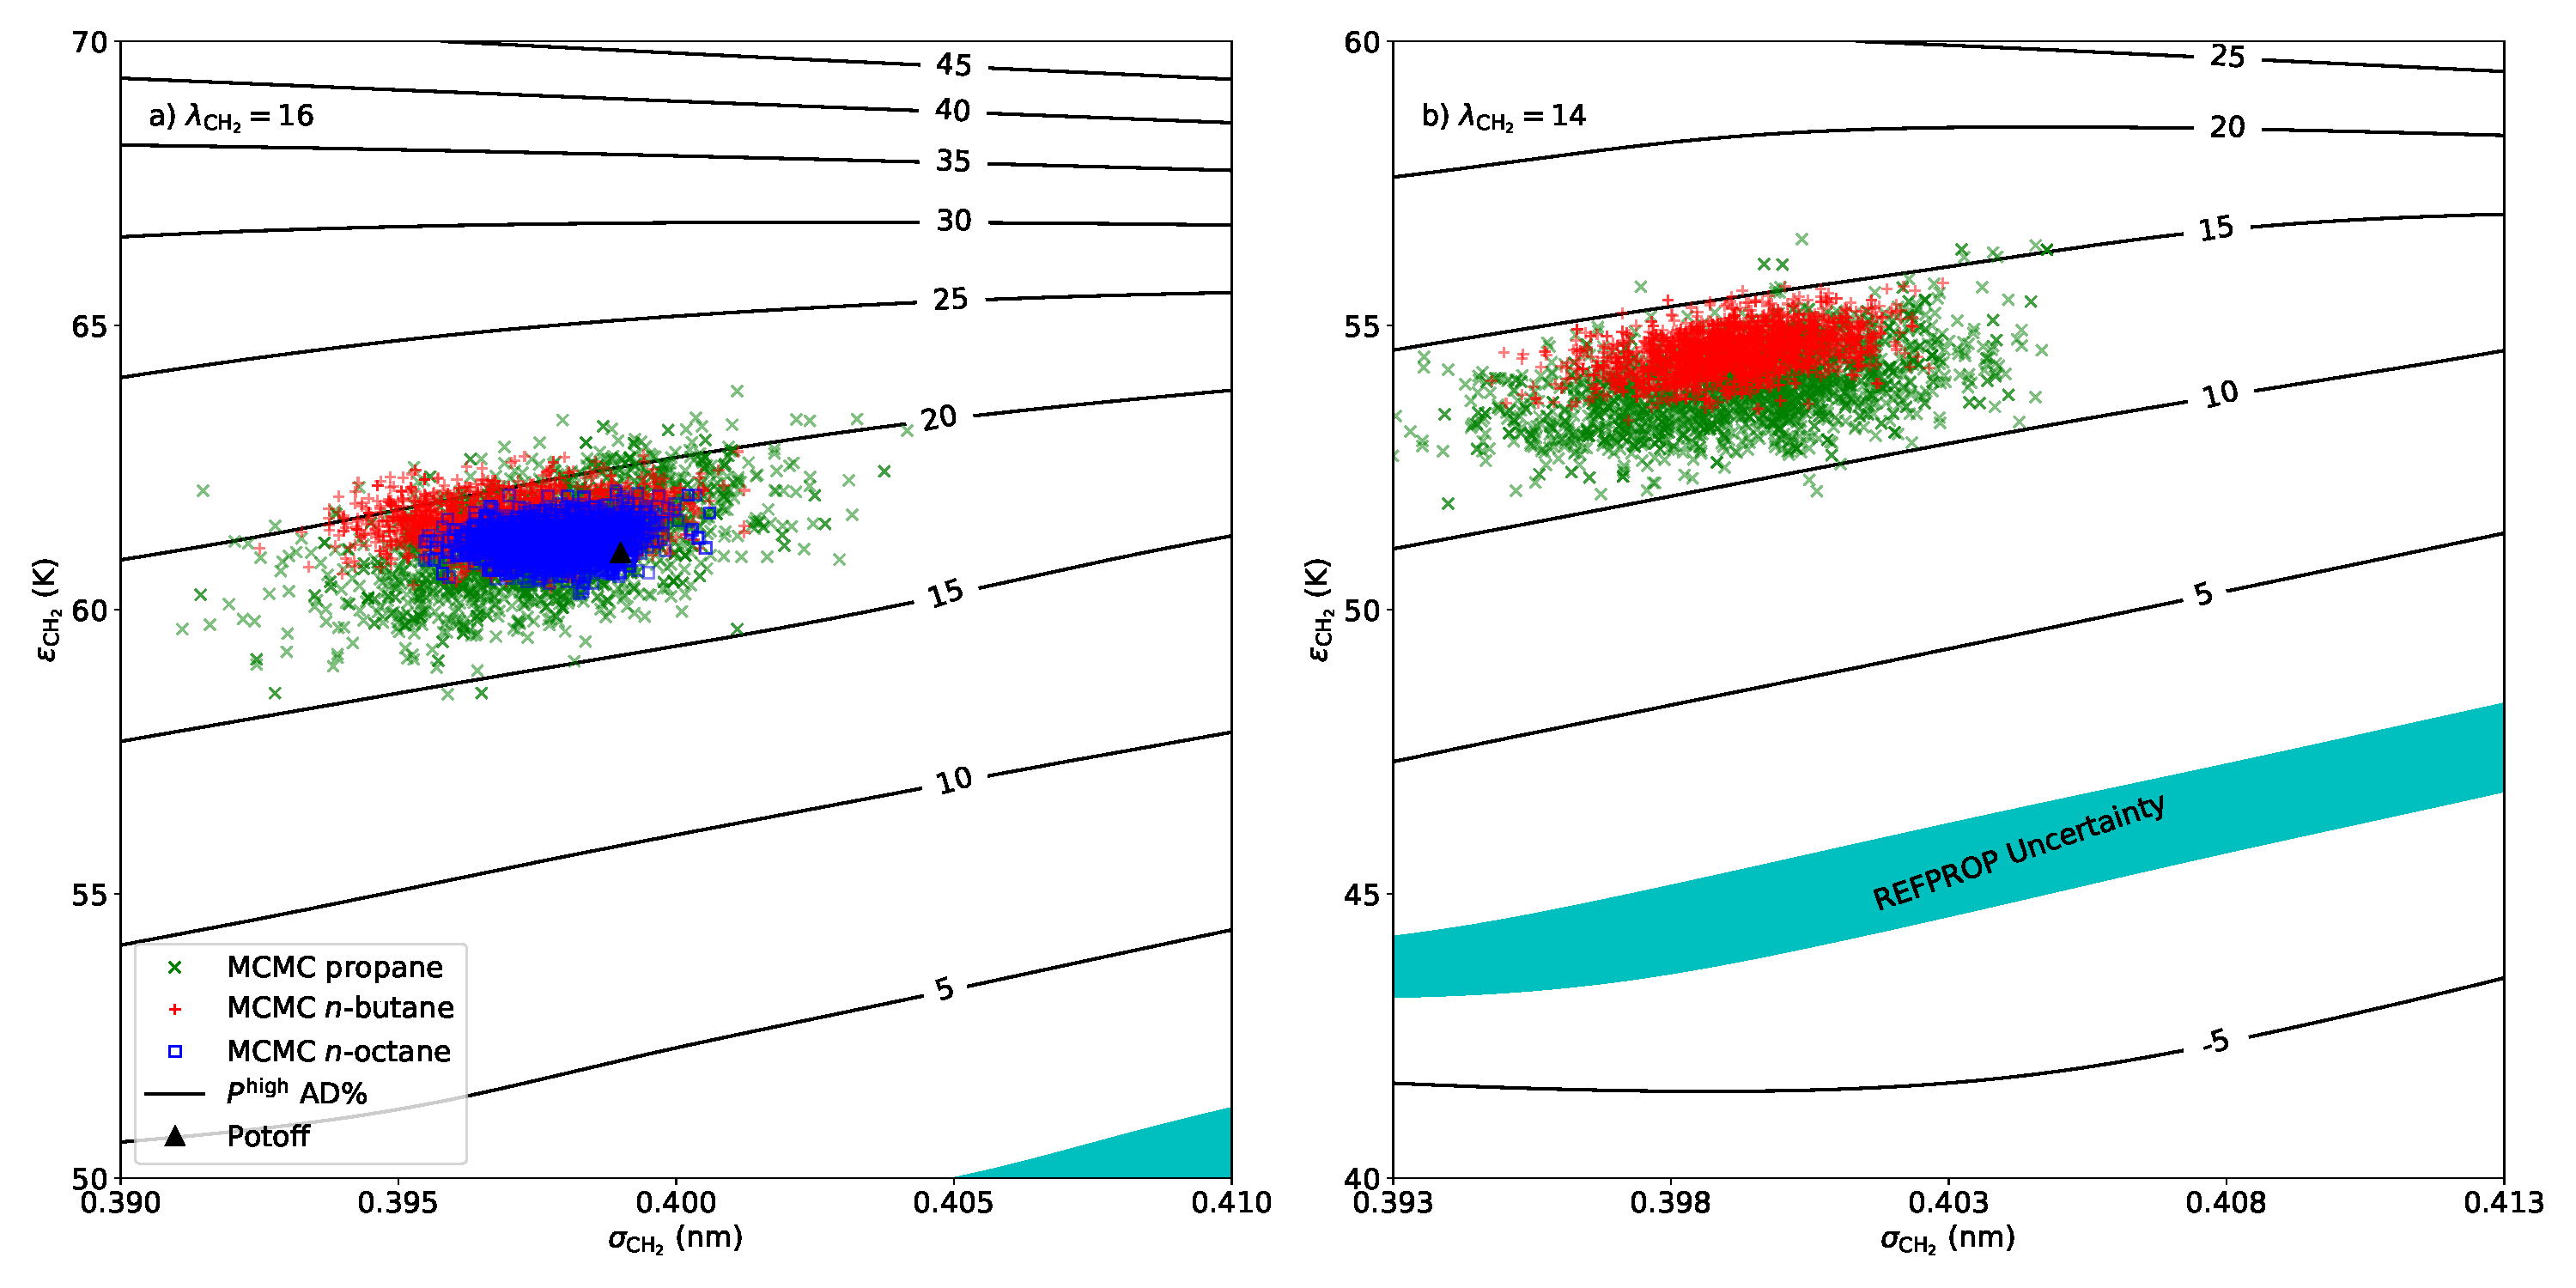
\includegraphics[width=6.4in]{MCMC_Mie_14_16_propane_butane_octane}
%MRS2: is blue missing on lam=14? Make sure in same order, maybe make more translucent.
%RAM2: lam=14 did not have results for octane yet. I have those running right now. Should be done by April 2.
	\caption{MCMC sampled $\epsilon_{\rm CH_2}$ and $\sigma_{\rm CH_2}$ parameter sets result in large AD\% for $P^{\rm high}$. Panels a) and b) correspond to $\lambda_{\rm CH_2} = 16$ and $\lambda_{\rm CH_2} = 14$, respectively. Contours are the AD\% in $P^{\rm high}$ relative to the REFPROP correlations, where the ``REFPROP uncertainty'' region represents $\pm 1$\% deviation. Panel a) includes the Potoff parameter set as a reference for $\lambda_{\rm CH_2} = 16$.}
	\label{fig:MCMC_Mie_14_16_propane_butane_octane}
\end{figure} 

%Figure \ref{fig:MCMC_Mie16_propane_butane_octane} presents the MCMC sampled $\epsilon_{\rm CH_2}$ and $\sigma_{\rm CH_2}$ parameter sets with $\lambda_{\rm CH_2} = 16$. Notice that the MCMC sampled $\epsilon_{\rm CH_2}$ and $\sigma_{\rm CH_2}$ parameter sets overlap considerably for propane, \textit{n}-butane, and \textit{n}-octane. This supports the common assumption of transferability of CH$_2$ parameters between different \textit{n}-alkanes. Note that the uncertainty in the parameters is largest for propane and smallest for \textit{n}-octane. This suggests that, as expected, the sensitivity of $\rho_{\rm l}^{\rm sat}$ and $P_{\rm v}^{\rm sat}$ with respect to the CH$_2$ parameters increases with increasing number of CH$_2$ interaction sites. Also, notice that the Potoff parameter set is within the MCMC sample region. More importantly, for the purposes of this manuscript, the MCMC sampled $\epsilon_{\rm CH_2}$ and $\sigma_{\rm CH_2}$ parameter sets have $P^{\rm high}$ AAD\% $\approx 16$-$23$, while the REFPROP uncertainty in $P^{\rm high}$ is estimated to be around $1$\%.

%\begin{figure}[htb!]
%	\centering
%	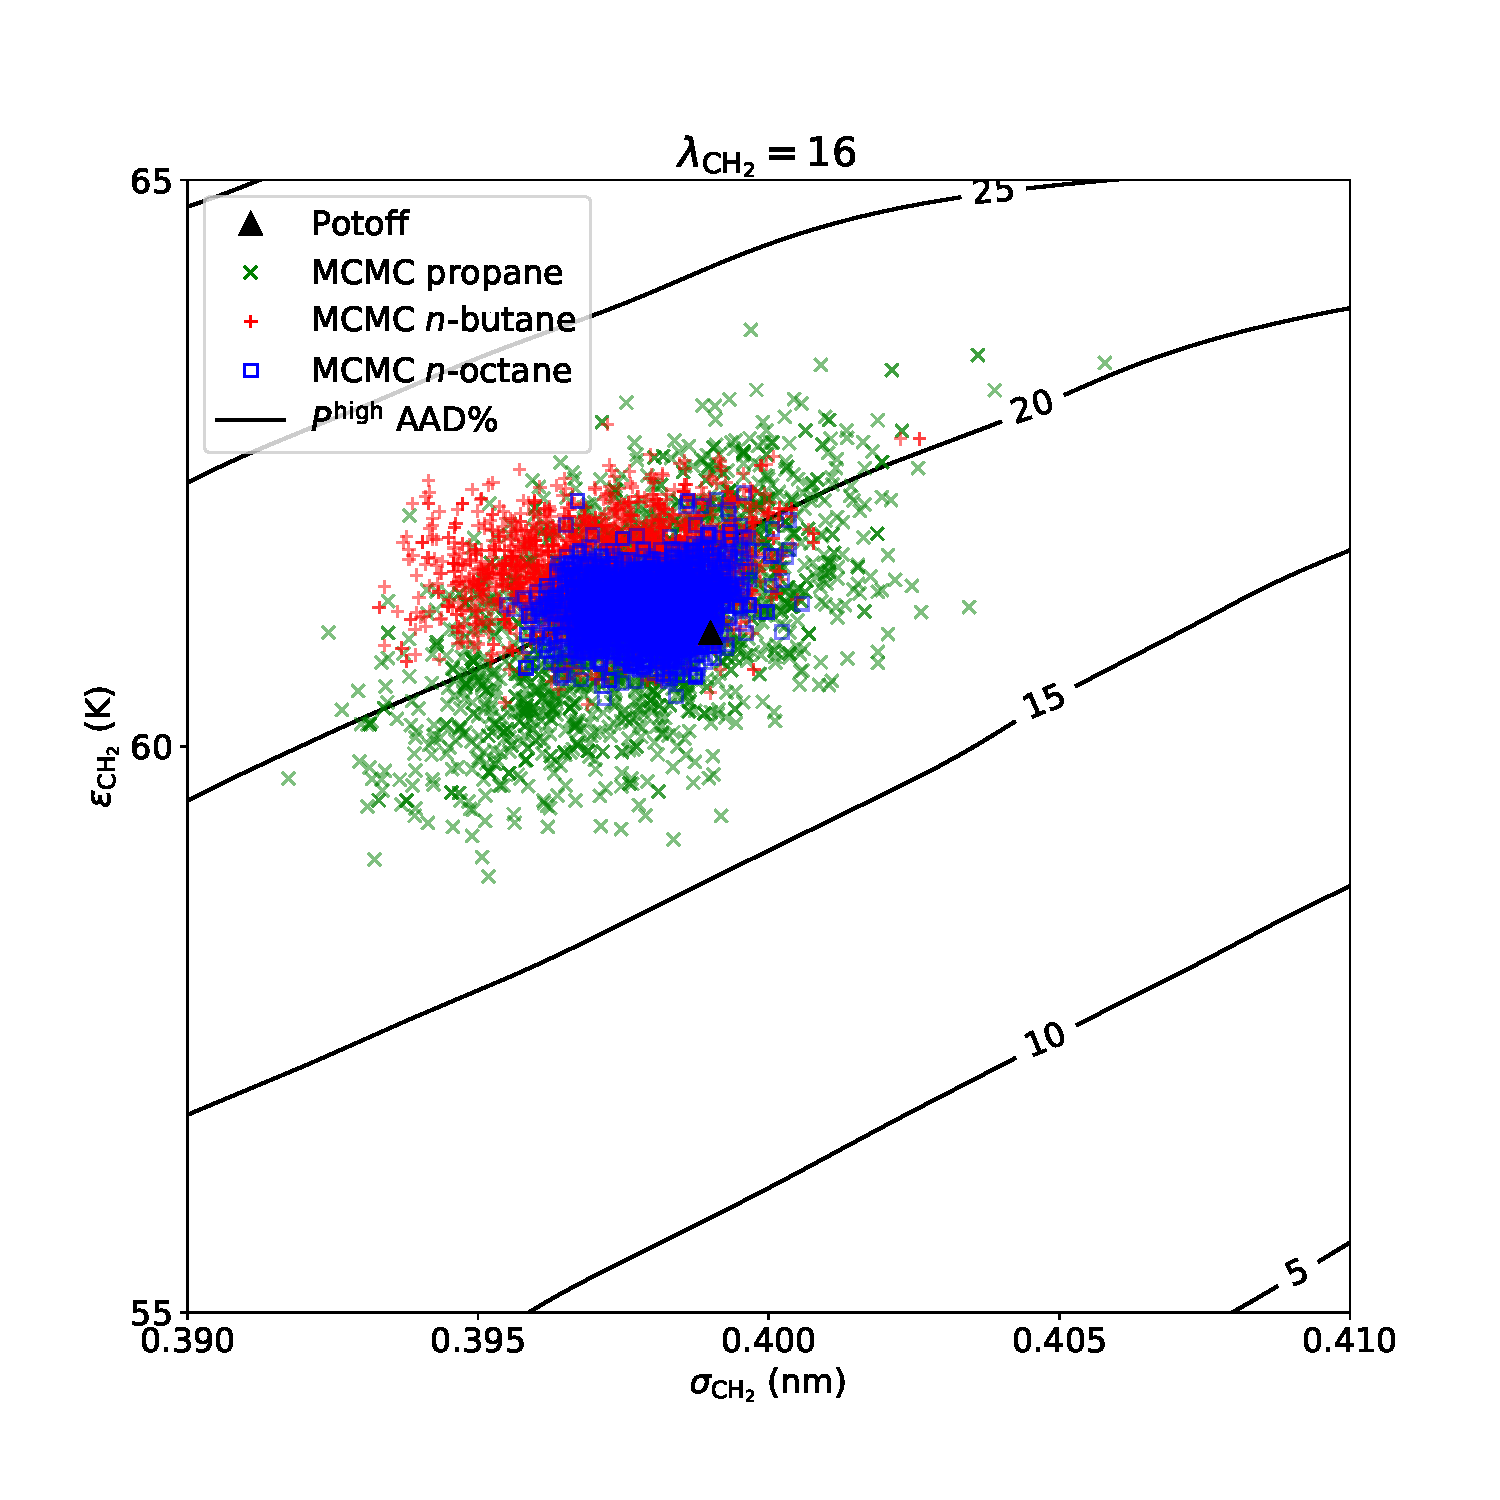
\includegraphics[width=3.2in]{MCMC_Mie16_propane_butane_octane}
%	\caption{MCMC sampled $\epsilon_{\rm CH_2}$ and $\sigma_{\rm CH_2}$ parameter sets with $\lambda_{\rm CH_2} = 16$ result in AAD\% $\approx 16$-$23$ for $P^{\rm high}$. REFPROP uncertainty in $P^{\rm high}$ is $\pm 1$\%. Potoff parameter set is provided as a reference.}
%	\label{fig:MCMC_Mie16_propane_butane_octane}
%\end{figure}

Notice in Figure \ref{fig:MCMC_Mie_14_16_propane_butane_octane} that the MCMC sampled $\epsilon_{\rm CH_2}$ and $\sigma_{\rm CH_2}$ parameter sets, for a given value of $\lambda_{\rm CH_2}$, overlap considerably for propane, \textit{n}-butane, and \textit{n}-octane. These joint-distributions provide statistical evidence in favor of the common assumption that CH$_2$ parameters are transferable between different \textit{n}-alkanes. To further demonstrate this point, Figure \ref{fig:MCMC_Mie_14_16_propane_butane_octane} includes the MCMC results when the posterior is based on the combined likelihoods from all three compounds, referred to as ``MCMC transferable.''

Panel a) shows that the Potoff CH$_2$ parameter set is within the MCMC sample regions for $\lambda_{\rm CH_2} = 16$. The same result was also observed for ethane (see Figure \ref{fig:MCMC_ethane_parameter_space}). This suggests that the Potoff CH$_3$ and CH$_2$ parameters are supported by the VLE data used in this study, even though the Potoff force field was parameterized using VLE data in a higher temperature range $(0.6 < T_{\rm r}^{\rm sat} < 0.95)$. 
%MRS2: ``likely parameter sets'' or ``parameter sets supported by data''?
%RAM2: Done
%feasible parameter sets.

Also, note that the uncertainty in the parameters is largest for propane and smallest for \textit{n}-octane. Therefore, the sensitivity of $\rho_{\rm l}^{\rm sat}$ and $P_{\rm v}^{\rm sat}$, with respect to the CH$_2$ parameters, increases with increasing number of CH$_2$ interaction sites. Although this result is fairly intuitive, it is a valuable insight when selecting a training set of molecules for force field development. For example, notice that the MCMC transferable region is almost identical to that of \textit{n}-octane, which shows that propane and \textit{n}-butane data provide relatively little additional information that is not contained in the \textit{n}-octane data. 

%%% Considering moving these two paragraphs higher since they are the main conclusions
%MRS3: first sentence isn't really a conclusion, make more direct?
Most importantly, for the purposes of this study, the contours in Figure \ref{fig:MCMC_Mie_14_16_propane_butane_octane} demonstrate that 
%For the purposes of this study, it is important to focus on the contours in Figure \ref{fig:MCMC_Mie_14_16_propane_butane_octane}, which correspond to AD\% in $P^{\rm high}$. 
%Notice that 
the MCMC sampled $\epsilon_{\rm CH_2}$ and $\sigma_{\rm CH_2}$ parameter sets have a strong positive bias (i.e. large AD\%) in $P^{\rm high}$. Specifically, $\lambda_{\rm CH_2} = 16$ and $\lambda_{\rm CH_2} = 14$ have, respectively, AD\% of $\approx 16$-$21$ and $\approx 10$-$15$, much greater than the REFPROP uncertainty of around $1$\%. 
Furthermore, because the 0\% contour is roughly parallel to the MCMC region and found at much lower $\epsilon_{\rm CH_2}$ values, it is necessary to sacrifice considerable accuracy in $\rho_{\rm l}^{sat}$ and $P_{\rm v}^{\rm sat}$ in order to accurately predict $P^{\rm high}$. 
It is interesting that, for corresponding values of $\lambda$, the AD\% for these larger \textit{n}-alkanes is higher than that of ethane. This suggests that longer chain-lengths, with a UA Mie $\lambda$-6 force field, exacerbate the erroneous $Z$ trend at high pressures.

% for the UA Mie $\lambda$-6 potential   

Although the AD\% in $P^{\rm high}$ is slightly lower for $\lambda_{\rm CH_2} = 14$ than for $\lambda_{\rm CH_2} = 16$, the UA Mie 14-6 potential is significantly less reliable for VLE. Figure \ref{fig:Bayes_Factors} demonstrates that there is ``strong'' evidence for $\lambda_{\rm CH_2} = 16$ over $\lambda_{\rm CH_2} = 14$, based on VLE data. 
%MRS2: sentences shouldn't be parenthetical.
%RAM2: Done
%MRS3: phrased correctly below?  Should be evidence for a property of CH2 and CH3.
%RAM3: Phrased correctly but not clearly. Tried to be more explicit.
Note that the evidence in Figure \ref{fig:Bayes_Factors} for the $\lambda$ value of CH$_2$ sites is stronger than that for the CH$_3$ sites. This suggests that the ethane $\rho_{\rm l}^{sat}$ and $P_{\rm v}^{\rm sat}$ results are less sensitive to $\lambda$ than the larger \textit{n}-alkanes and/or that the ethane VLE data contains less information than the combined data of propane, \textit{n-butane}, and \textit{n}-octane.
% three larger \textit{n}-alkanes. 
% because VLE data from more than one compound were included. 
%Furthermore, because the ``REFPROP uncertainty'' contours are roughly parallel to the MCMC region and found at much lower $\epsilon_{\rm CH_2}$ values, it is necessary to sacrifice considerable accuracy in $\rho_{\rm l}^{sat}$ and $P_{\rm v}^{\rm sat}$ in order to accurately predict $P^{\rm high}$. 
In conclusion, these results suggest that neither UA Mie 16-6 or 14-6 force fields are capable of predicting VLE and $P \rho T$ for supercritical fluids and compressed liquids of \textit{n}-alkanes. 

%Therefore, considering the deprecation in VLE, the marginal gain in accuracy for $P^{\rm high}$ does not merit using a UA Mie 14-6 potential.

% Therefore, Figure \ref{fig:MCMC_Mie_14_16_propane_butane_octane} provides convincing evidence that, regardless of the value of $\lambda$, the UA Mie $\lambda$-6 model is not capable of predicting both VLE and $P \rho T$ at high pressures.

%The REFPROP uncertainty region that corresponds to AAD\% of $\pm 1$ is parallel to the MCMC region and found at much lower $\epsilon_{\rm CH_2}$ (around 45 K for the same $\sigma_{\rm CH_2}$). Therefore, in order to accurately predict $P^{\rm high}$, it is necessary to sacrifice accuracy in $\rho_{\rm l}^{sat}$ and $P_{\rm v}^{\rm sat}$. Figures \ref{fig:MCMC_Mie16_propane_butane_octane}-\ref{fig:MCMC_Mie14_propane_butane} provide convincing evidence that, regardless of the value of $\lambda$, the UA Mie $\lambda$-6 model is not capable of predicting both VLE and $P \rho T$ at high pressures.

%Also, notice that the MCMC sampled $\epsilon_{\rm CH_2}$ and $\sigma_{\rm CH_2}$ parameter sets overlap considerably for the two compounds. In other words, the $\epsilon_{\rm CH_2}$ and $\sigma_{\rm CH_2}$ parameter sets for propane and \textit{n}-butane are indistinguishable to within uncertainty. This supports the common assumption of transferability of CH$_2$ parameters between different \textit{n}-alkanes.

%Figure \ref{fig:MCMC_Mie16_propane_butane_octane} suggests that the UA Mie 16-6 potential is not capable of predicting VLE and $P \rho T$ for supercritical fluids and compressed liquids of propane, \textit{n}-butane, and \textit{n}-octane. Figure \ref{fig:MCMC_Mie14_propane_butane} demonstrates that the UA Mie 14-6 potential is also not capable of predicting both properties for propane and \textit{n}-butane. Specifically, all of the MCMC sampled $\epsilon_{\rm CH_2}$ and $\sigma_{\rm CH_2}$ parameter sets in Figure \ref{fig:MCMC_Mie14_propane_butane} have $P^{\rm high}$ AAD\% $\approx 10$-$15$. Although this is improvement relative to the UA Mie 16-6 AAD\%, recall that the UA Mie 14-6 is less reliable for VLE. Therefore, considering the significant deprecation in VLE, the marginal gain in accuracy for $P^{\rm high}$ likely does not merit using a UA Mie 14-6 potential. 
%
%Figure \ref{fig:MCMC_Mie14_propane_butane} also includes the ``REFPROP uncertainty'' region which corresponds to AAD\% of $\pm 1$.  Because the ``REFPROP uncertainty'' contours are parallel to the MCMC region and found at much lower $\epsilon_{\rm CH_2}$ (around 45 K for the same $\sigma_{\rm CH_2}$), in order to accurately predict $P^{\rm high}$, it is necessary to sacrifice accuracy in $\rho_{\rm l}^{sat}$ and $P_{\rm v}^{\rm sat}$. Figures \ref{fig:MCMC_Mie16_propane_butane_octane}-\ref{fig:MCMC_Mie14_propane_butane} provide convincing evidence that, regardless of the value of $\lambda$, the UA Mie $\lambda$-6 model is not capable of predicting both VLE and $P \rho T$ at high pressures.

%\begin{figure}[htb!]
%	\centering
%	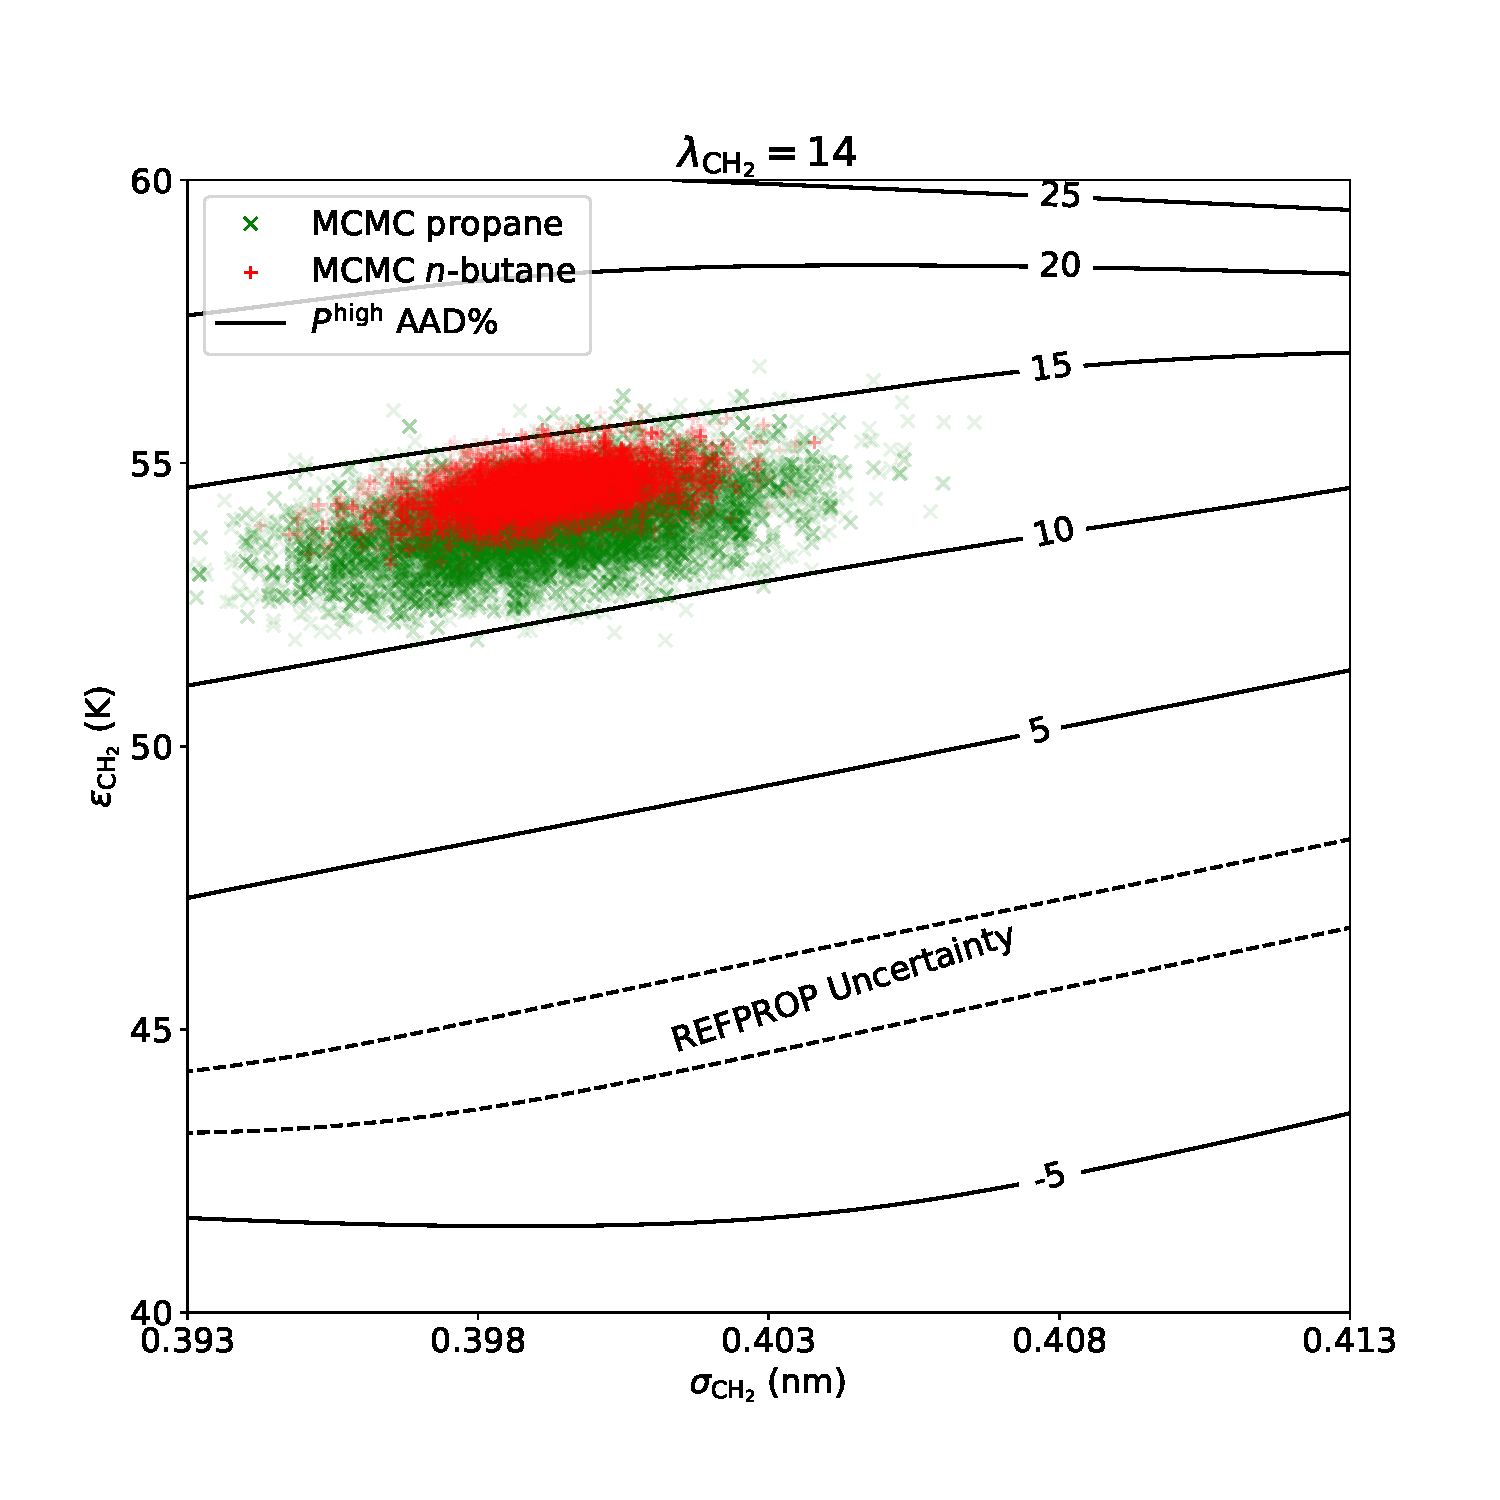
\includegraphics[width=3.2in]{MCMC_Mie14_propane_butane}
%	\caption{MCMC sampled $\epsilon_{\rm CH_2}$ and $\sigma_{\rm CH_2}$ parameter sets with $\lambda_{\rm CH_2} = 14$ result in AAD\% $\approx 10$-$15$ for $P^{\rm high}$. REFPROP uncertainty in $P^{\rm high}$ is included at $\pm 1$\%.}
%	\label{fig:MCMC_Mie14_propane_butane}
%\end{figure}

%\begin{enumerate}
%	\item Figure: The uncertainty regions for CH3, CH2, CH, and C. I can include 14-6, 15-6, and 16-6. Perhaps I will only do this rigorous analysis for CH3 or for CH3 and CH2. Probably not for all. 
%%MRS: might be weaker to say it's a rigorous bayesian analysis if only done for 2; people could always say ``but maybe it will work for C and CH'', though obviously, it C and CH parmeters are irrelevant for n-alkanes.  
%%MRS: so one could optimize CH3 and CH2, and then optimize for C and CH given CH2 and CH3. Importantly, you can back-calcuate the confidence regions for different CH2 and CH3 parameters for n-alkanes, alone, since that just affects the posteriors when adding C and CH data.  
%%MRS: is the reason not for all the computational expense?
%%MRS: it could be with the constraints on CH2 and CH3 from the n-alkanes, you can do a restricted 3D search with CH (not bothering to do already low probability regions of CH3 and CH3, and then do a restricted 4D search with the constraints on CH3/CH2/CH''.  Not many molecules that have C and CH, so fewer simulations to do.  
%%MRS: or could just say ``doesn't work for normal, so no point in worrying about C and CH''.
%I could include the results from the alternative posterior (excluding Pvsat and including high pressures) but then it might be out of place in this section.
%	\item Bayes factors demonstrate that, for VLE, a 15-6 or 16-6 potential are favored significantly more than a 14-6 (could include 17-6 or 18-6 as well)
%%MRS: probably want to go until the probability turns down again. 
%	\item CH2 credible regions overlap considerably between propane, n-butane, and n-octane
%%MRS: You want to show the combined region as well, though; muliplying the probabilities. 
%%MRS: Do you want to include data showing that separate CH2 and CH3 parameters are necessary? Would be nice to use Bayesian analysis to show more dimensions are necessary. Is that already established?  Might be a nice way to demonstrate Bayesian approach to show things already established like this.
%	\item By comparing the Bayes factor of a transferable CH2 site and three independent CH2 sites we observe that the CH2 sites are indistinguishable
%	\item Statement about CH credible regions for isobutane, isopentane, and isohexane
%	\item Statement about C credible region for isooctane and neopentane
%\end{enumerate}

%\subsection{Propagation of uncertainties}

% I am not sure where this should go. Perhaps supporting information?
%\begin{enumerate}
%%MRS: be more precise about what you mean by propagation of uncertainties. 95% confidence intervals?  Standard deivations? What is the point that you are proving with this data?
%	\item Figure: Uncertainties in rholsat and Pvsat for n-alkanes. Include 14-6, 15-6, 16-6.
%	\item Figure: Uncertainties in rholsat and Pvsat for branched alkanes. Include only 16-6.
%	\item Clearly the uncertainties are fairly conservative due to the relatively large numerical uncertainties we assigned in the posterior
%%MRS: Not clear; uncertainties in rholsat and Pvsat affect the posterior . . . ? Important point; the way that we've defined likelihood includes the experimental uncertainty, but not the numerical uncertainty. 
%	\item Figure: Z vs 1000/T for n-alkanes where the error bars represent the Bayesian uncertainties from VLE. Include 14-6, 15-6, and 16-6 results.
%%MRS: for the points below, what is the proof of the points; the figure of Z vs 1000/T? Be clear.
%	\item The 16-6 potential is not able to predict both VLE and compressed liquid/supercritical pressures
%	\item VLE is much worse for 14-6, about the same for 15-6
%	\item Condensed liquid pressures are slightly better for 14-6 and 15-6 but still over-predict
%	\item Figure: Z vs 1000/T for branched alkanes. Results are only included for the 16-6 potential.
%	\item Same results as for normal alkanes.
%\end{enumerate}

%%% RAM: We feel like this discussion could just be a paragraph saying that if Pvsat is not important you could use a 14-6 potential and match just liquid phase pressures
%\subsection{Optimal $\lambda$ for high pressures}
%MRS: might need to justify why or why not would would need Pvstat.
%\begin{enumerate}
%	\item We modify the posterior by excluding the Pvsat data and including the REFPROP correlations at high pressures
%	\item Figure: I can either include the parameter uncertainties here or back in the Parameter Uncertainties section. I could even move this to supporting information
%	\item Bayes ratios show the evidence for different values of $\lambda$
%	\item We recommend that lower values of $\lambda$ be favored
%%MRS: but the thesis is that MIE isn't sufficient; difficult if you are complicating the thesis too much.
%\end{enumerate}

\section{Discussion} \label{Discussion} 

\subsection{Recommendations} \label{Recommendations}

%The Mie $\lambda$-6 potential is capable of reproducing $\rho_{\rm l}^{\rm sat}$ and $P_{\rm v}^{\rm sat}$ for $\lambda = 15$ or $16$. Unfortunately, this improved accuracy does not appear to have physical/theoretical justification. For this reason, $\lambda$ values greater than $13$ over-predict pressures for supercritical fluids and compressed liquids. 

%Therefore, for developing FEOS of normal and branched alkanes, we 
%%MRS2: can you recommended them if you didn't run them?  Perhaps something like ``further investigation should look at alternative . . . ``
%%RAM2: Done
%recommend further investigation of alternative potentials with a softer repulsive barrier and a more sound theoretical basis, e.g. Buckingham exponential-6, Morse \cite{Rowley1999,Rowley2001,Hayes2004}, or an extended Lennard-Jones \cite{Mostafa_Diss,Hajigeorgiou2016,Kalos1972}.

Although the UA Mie $\lambda$-6 potential is not quantitatively reliable at high pressures, it may still be of use for FEOS parameterization when considering the insight gained in this study. For example, since the Potoff force field consistently over-predicts high pressures, a non-linear FEOS optimization could utilize the simulation results as an upper constraint for the FEOS pressure \cite{Thol_LJTS}. Furthermore, the primary purpose to include molecular simulation data for FEOS development is to increase the range of validity by ensuring good behavior of the FEOS at high temperatures and pressures. While FEOS are based on empirical equations with $15$--$30$ fitting parameters, even an inaccurate force field has a more sound theoretical basis. Therefore, the UA Mie $\lambda$-6 simulation output for a given property should not demonstrate non-physical oscillations, inflection points, derivative sign-changes, etc., which can plague a poorly-fit FEOS.

%It remains to be seen if improvement in FEOS extrapolation is possible for an FEOS is possible , it remains to be seen if the UA Mie $\lambda$-6 potential can 
%
%% the derivative of a given property. Therefore, since molecular simulation results with the UA Mie $\lambda$-6 potential should not demonstrate non-physical oscillations, inflection points, or sign-changes for the derivative of a given property,  a change in the derivative sign. 
%
% divergence at conditions outside of the training set
%
%
% Despite the systematic deviations at high pressures, the UA Mie $\lambda$-6 results should not diverge . 

%The primary purpose to include molecular simulation data for FEOS development is to increase the range of validity by ensuring good behavior of the FEOS at high temperatures and pressures.

Essentially, whether or not a FEOS should be developed using a hybrid data set consisting of UA Mie $\lambda$-6 simulation results depends on the quality and quantity of available experimental data. If the data cover a wide range of state points and properties, it is possible that the UA Mie $\lambda$-6 potential may still be useful, despite the systematic deviations at high pressures. By contrast, if the experimental data are limited such that the FEOS depends almost entirely on the molecular simulation results, the UA Mie $\lambda$-6 force field will lead to large deviations at high pressures. Therefore, in this scenario, we advise against the use of UA Mie $\lambda$-6 force fields when developing a FEOS for normal and branched alkanes. For this purpose, 
% for developing FEOS of normal and branched alkanes, we 
%MRS2: can you recommended them if you didn't run them?  Perhaps something like ``further investigation should look at alternative . . . ``
%RAM2: Done
we recommend further investigation of alternative potentials with a softer repulsive barrier and a more sound theoretical basis, e.g. Buckingham exponential-6, modified-Morse \cite{Rowley1999,Rowley2001,Hayes2004}, or an extended Lennard-Jones \cite{Mostafa_Diss,Hajigeorgiou2016,Kalos1972}.

% It remains to be seen if the UA Mie $\lambda$-6 potential can still provide a reasonable trend, despite the systematic deviations at high pressures, to help keep the FEOS from diverging.  

%Thus, despite our findings that the UA Mie $\lambda$-6 potential is not quantitatively reliable at high pressures, it remains to be seen if this potential can be used in a hybrid data set.

%However, despite our findings that the UA Mie $\lambda$-6 potential is not quantitatively reliable at high pressures, it remains to be seen if this potential can be used in a hybrid data set. The primary purpose to include molecular simulation data for FEOS development is to increase the range of validity by ensuring good behavior of the FEOS at high temperatures and pressures. Therefore, although the Mie 16-6 over-predicts pressure, it still provides a reasonable trend to help keep the FEOS from diverging. In addition, since the Mie 16-6 potential consistently over-predicts pressure, it is possible to use the simulation results as an upper constraint. 

\subsection{Limitations} \label{Limitations}

%MRS2: the purpose of this section is not too clear.
%RAM2: Included a sentence to explain why this is important
%The simulation values that are typically included in hybrid data sets are derivatives of the residual Helmholtz free energy $(\partial^n a^{\rm r})$ with respect to inverse temperature and/or density \cite{Thol2016_siloxane_first,Thol2016_siloxane,Thol2017}, while in this study we simply compare the $P \rho T$ behavior. Aside from the advantage of simplicity (most simulation packages do not provide $\partial^n a^{\rm r}$), this choice is based on the fact that $P \rho T$ is more readily understood and easier to visualize. In other words, it is easier to quantify the impact on process design caused by deviations in $P \rho T$ behavior than derivatives in the residual Helmholtz free energy. Furthermore, as demonstrated by Thol et al., an inaccurate prediction of some $\partial^n a^{\rm r}$ does not necessarily result in poor prediction of $P \rho T$ behavior or heat capacities \cite{Thol2016_siloxane_first}. 
%
%It is important to remember that $Z$ depends only on the first derivative of Helmholtz free energy with respect to density. $U^{\rm dep}$ is linearly dependent on the first derivative of residual Helmholtz free energy with respect to inverse temperature. From our analysis we also observed some systematic bias in $U^{\rm dep}$ at high pressures. Unfortunately, deficiencies in the $U^{\rm dep}$ trends are not as obvious due to the relatively large uncertainties in the REFPROP correlations, ca. 5\%. While $Z$ and $U^{\rm dep}$ directly impact FEOS parameterization, this study does not assess the quality of the Mie $\lambda$-6 potential for the other four derivatives. Therefore, future work should investigate the adequacy of force fields to predict heat capacities, which depend on temperature derivatives, at higher temperatures and pressures. Rigorous studies of this type have been performed on the single-site Lennard-Jones fluid \cite{Thol2016_LJ,Thol_LJTS,Rutkai2017}. 
%
%We would like to emphasize that, although we did not use $\partial^n a^{\rm r}$ for our analysis, including higher order derivatives of the residual Helmholtz free energy from molecular simulation has significant advantages for developing FEOS as it eliminates redundant information found in traditional macroscopic properties \cite{Thol2016_LJ,Thol_LJTS,Rutkai2017,Lustig2015,Rutkai2013,Rutkai2015}. Since $Z$ and $U^{\rm dep}$ depend on only a single derivative and are readily available for most simulation packages, we chose to investigate these properties.

This section discusses limitations to the primary conclusion from this study, namely, that UA Mie $\lambda$-6 force fields parameterized with VLE data should not be used to develop fundamental equations of state for normal and branched alkanes. The main limitation is that the poor extrapolation at high pressures is based solely on the trend of $Z$ with respect to inverse temperature. By contrast, the simulation values that are typically included in hybrid data sets are derivatives of the residual (or departure) Helmholtz free energy with respect to inverse temperature and/or density \cite{Thol2016_siloxane_first,Thol2016_siloxane,Thol2017,Rutkai2013,Thol2015}:
\begin{equation} \label{Residual Derivatives}
A_{xy}^{\rm dep} R_gT \equiv (1/T)^x\rho^y \frac{\partial^{x+y}A^{\rm dep}}{\partial(1/T)^x \partial \rho^y}
\end{equation}
We would like to emphasize the advantage of using $A_{xy}^{\rm dep}$ for developing FEOS, as this approach eliminates redundant information found in traditional macroscopic properties \cite{Thol2016_LJ,Rutkai2017,Lustig2015,Rutkai2013,Rutkai2015}. For example, the following expressions demonstrate the interdependency of the properties we computed, namely, $Z$ and $U^{\rm dep}$ with their derivatives along isochores and isotherms \cite{Rutkai2015}:
\begin{equation} \label{eq:Z}
Z = 1 + A_{01}^{\rm dep}
\end{equation}
\begin{equation} \label{eq:Z_IC}
\frac{1}{T} \left(\frac{-\partial Z}{\partial(1/T)}\right)_\rho = 1 + A_{01}^{\rm dep} - A_{11}^{\rm dep}
\end{equation}
\begin{equation} \label{eq:U}
\frac{U^{\rm dep}}{R_gT} = A_{10}^{\rm dep}
\end{equation}
\begin{equation} \label{eq:U_IC}
\frac{1}{R_g} \left(\frac{\partial U^{\rm dep}}{\partial T}\right)_\rho = -A_{20}^{\rm dep} 
\end{equation} 
\begin{equation} \label{eq:Z_IT}
\rho \left(\frac{\partial Z}{\partial \rho}\right)_T = 1 + 2 A_{01}^{\rm dep} + A_{02}^{\rm dep} 
\end{equation}
Unfortunately, with the exception of \textit{ms2} \cite{ms2}, we are not aware of any open-source simulation package that readily provides $A_{xy}^{\rm dep}$. 
%MRS2: this is something we can set up relatively easily for OpenFF (along with the similar derivatives for NPT), and perhapsshould.  Owen has been working along these lines.
%RAM2: I assume you mean OpenMM?

In addition, macroscopic properties, such as $Z$ and $U^{\rm dep}$ (with their respective derivatives), are more readily understood and visualized than $A_{xy}^{\rm dep}$. Also, it is easier to quantify their impact on process design than derivatives in the residual Helmholtz free energy. For example, as demonstrated in 
%MRS3: check if there is a way to cite the number not superscripted.
%RAM3: Should have used \citenum not \cite
Reference \citenum{Thol2016_siloxane_first}, an inaccurate prediction of some $A_{xy}^{\rm dep}$ does not necessarily result in poor prediction of $P \rho T$ behavior or heat capacities. For these reasons, we did not base our conclusions on the adequacy of the UA Mie $\lambda$-6 potential to predict $A_{xy}^{\rm dep}$.

Instead, we have presented $Z$ and, by inspection, the slope of $Z$ with respect to $1/T$ at constant $\rho$. Since these properties are equivalent to Equations \ref{eq:Z}-\ref{eq:Z_IC}, respectively, we have indirectly focused on only two of the Helmholtz derivatives, namely, $A_{01}^{\rm dep}$ and $A_{11}^{\rm dep}$. However, we also observed some deviations in $U^{\rm dep}$, the slope of $U^{\rm dep}$ with respect to $T$ at constant $\rho$, and the slope of $Z$ with respect to $\rho$ at constant $T$, which are equivalent to Equations \ref{eq:U}-\ref{eq:Z_IT}. Unfortunately, deficiencies are not as obvious for these properties due to the relatively large uncertainties in the REFPROP correlations, ca. 5\% and 10\% for $U^{\rm dep}$ and $\left(\frac{\partial U^{\rm dep}}{R_g \partial T}\right)_\rho$. Although these additional properties provide insight regarding $A_{10}^{\rm dep}$, $A_{20}^{\rm dep}$, $A_{01}^{\rm dep}$, and $A_{02}^{\rm dep}$, because the results are less conclusive they are provided only in Section \ref{Udep and Z_IT} of Supporting Information. Furthermore, the relationship between Equations \ref{eq:U}-\ref{eq:Z_IT} and the repulsive barrier, $\lambda$, is not obvious. By contrast, the observation that larger values of $\lambda$ over-predict $Z$ with increasing temperature is clear evidence that $\lambda > 12$ is not theoretically justified but, rather, is an empirical remedy that performs well for VLE.

Future work should investigate more thoroughly the adequacy of UA Mie $\lambda$-6 (or other) force fields to predict $U^{\rm dep}$ and isochoric/isobaric heat capacities at high temperatures and pressures. For example, rigorous studies of this type have been performed on the single-site Lennard-Jones fluid \cite{Thol2016_LJ,Thol_LJTS,Rutkai2017}.  

Another limitation is that we utilize a single layer Bayes model as opposed to a hierarchical model, where the posterior is proportional to multiple priors that depend on the parameters from different levels of the hierarchy (for a more detailed discussion see References \citenum{Kulakova2017,Wu2016}). Wu et al. demonstrated the need for hierarchical models when the data set, $D$, contains discrepancies, i.e. internal inconsistencies. 
%MRS3: why is it important?  Can you be more precise? What do you mean by discrepancies in the data set?
%RAM3: Provided a short explanation
Fortunately, since we use a conservative estimate for the surrogate model uncertainty, i.e. $u_{\rm SM} \gg u_{\rm D}$, any discrepancies in the VLE data should not affect the parameter uncertainties. 

%MRS3: not clear you've defined what you mean by hierarchical approach.  This paragrph is rather unclear, and will be worse for people without a lot of familiarity with Bayesian inference.
%RAM3: True, this discussion was mainly intended for those that are familiar with Bayesian inference. I do not think I have the space or capability to explain hierarchical models in simple terms. So I am just trying to explain why they would be needed. But I tried to provide a brief explanation
The hierarchical approach is also useful when accounting for model inadequacies, i.e. when the force field is not capable of representing multiple data types. A hierarchical method should thus be favored if determining the parameter uncertainty when simultaneously considering $\rho_{\rm l}^{\rm sat}$, $P_{\rm v}^{\rm sat}$ and $P^{\rm high}$. Furthermore, a hierarchical model should be used if the parameters are not transferable between molecules, i.e. if the CH$_2$ parameters were different for propane, \textit{n}-butane, and \textit{n}-octane. However, the hierarchical approach is unnecessary for our purposes, since the transferable UA Mie $\lambda$-6 force field for \textit{n}-alkanes is capable of reproducing $\rho_{\rm l}^{\rm sat}$ and $P_{\rm v}^{\rm sat}$, which are the only properties included in $D$. 

%In addition, hierarchical Bayesian models require a higher dimensionality that can be considerably more expensive computationally than a single layer model.

%The posterior propagation of uncertainty to $P^{\rm high}$ does not require.

%the purpose of this study is to demonstrate that, for all feasible parameter sets obtained from VLE properties, a UA Mie $\lambda$-6 force field is inaccurate for $P^{\rm high}$. Therefore, since we focus on the parameter uncertainty obtained from just $\rho_{\rm l}^{\rm sat}$ and $P_{\rm v}^{\rm sat}$, the hierarchical approach is unnecessary. In addition, hierarchical Bayesian models can be considerably more expensive computationally than a single layer model. 

%For these reasons, we utilized a single layer model to demonstrate that, for all feasible parameter sets obtained from VLE properties, a UA Mie $\lambda$-6 force field is inaccurate for $P^{\rm high}$.

%However, the purpose of this study is to demonstrate that, for all feasible parameter sets obtained from VLE properties, a UA Mie $\lambda$-6 force field is inaccurate for $P^{\rm high}$. 

%However, hierarchical models are not necessary to show that the UA Mie $\lambda$-6 potential is not capable of accurately predicting all three properties ($\rho_{\rm l}^{\rm sat}$, $P_{\rm v}^{\rm sat}$ and $P^{\rm high}$). Notice that we only included VLE data in our single layer Bayes model because the purpose of this study is to demonstrate that, for all feasible parameter sets obtained from VLE properties, a UA Mie $\lambda$-6 force field is inaccurate for $P^{\rm high}$. In addition, hierarchical Bayesian models are considerably more expensive computationally. For these reasons, we utilized the single layer Bayes methodology.

%Another limitation is that we utilize a single layer Bayes model as opposed to a hierarchical model \cite{Kulakova2017,Wu2016}. Wu et al. demonstrated that hierarchical models provide parameter uncertainties that more rigorously account for discrepancies in experimental data. Since $u_{\rm c} \gg u_{\rm exp}$, any discrepancies in the VLE data should not affect the parameter uncertainties. More importantly, the hierarchical approach is also useful when accounting for model inadequacies, i.e. when the force field is not capable of representing multiple data types. Therefore, the hierarchical method could determine the parameter uncertainty when simultaneously considering $\rho_{\rm l}^{\rm sat}$, $P_{\rm v}^{\rm sat}$ and $P^{\rm high}$. However, the purpose of this study is to demonstrate that, for all feasible parameter sets obtained from VLE properties, a UA Mie $\lambda$-6 force field over-predicts $P^{\rm high}$. In other words, hierarchical models are not necessary to show that no $\epsilon$, $\sigma$, and $\lambda$ set exists that is capable of accurately predicting all three properties ($\rho_{\rm l}^{\rm sat}$, $P_{\rm v}^{\rm sat}$ and $P^{\rm high}$). Furthermore, hierarchical Bayesian models are considerably more expensive computationally and were, therefore, not included in this study.

%Another limitation is that we have utilized a single layer Bayes model as opposed to a hierarchical model \cite{Kulakova2017,Wu2016}. Wu et al. demonstrated that hierarchical models can provide parameter uncertainties that more rigorously account for discrepancies in experimental data. Since $u_{\rm c} \gg u_{\rm exp}$, any discrepancies in the VLE data were non-consequential. Having said that, the hierarchical approach is useful when accounting for model inadequacies, i.e. when the force field is not capable of representing multiple data types. Therefore, the hierarchical method could determine the parameter uncertainty when simultaneously considering $\rho_{\rm l}^{\rm sat}$, $P_{\rm v}^{\rm sat}$ and $P^{\rm high}$. However, the purpose of this study is to demonstrate that a UA Mie $\lambda$-6 force field parameterized to VLE properties over-predicts $P^{\rm high}$, hierarchical models are not necessary to show that no set of $\epsilon$, $\sigma$, and $\lambda$ are capable of predicting all three properties. Furthermore, hierarchical Bayesian models are considerably more expensive computationally and were, therefore, not included in this study.

% More importantly, the purpose of this study is not to provide the feasible range of parameters, but rather to demonstrate that the VLE uncertainties  since $u_{\rm c} \gg u_{\rm exp}$,    

%For example, the following expressions relate $A_{xy}^{\rm dep}$ to the properties we computed in this study, namely, $U^{\rm dep}$ and $Z$ along isochores and isotherms:
%\begin{equation} \label{eq:Z}
%Z = 1 + A_{01}^{\rm dep}
%\end{equation}
%\begin{equation} \label{eq:Z_IC}
%-\frac{\partial Z}{T\partial(1/T)}_\rho = 1 + A_{01}^{\rm dep} - A_{11}^{\rm dep}
%\end{equation}
%\begin{equation} \label{eq:Z_IT}
%\frac{\rho \partial Z}{\partial \rho}_T = 1 + 2 A_{01}^{\rm dep} + A_{02}^{\rm dep} 
%\end{equation}
%\begin{equation} \label{eq:U}
%\frac{U^{\rm dep} }{R_gT} = A_{10}^{\rm dep}
%\end{equation}
%\begin{equation} \label{eq:U_IC}
%\frac{\partial U^{\rm dep}}{R_g \partial T}_\rho = -A_{20}^{\rm dep} 
%\end{equation}

%The conclusion regarding the adequacy of the UA Mie $\lambda$-6 potential at high pressures has been based on the trends observed for $Z$ along the isochores. In other words, we have focused on Equations \ref{eq:Z}-\ref{eq:Z_IC}, namely, $Z$ and the slope of $Z$ with respect to $(1/T)$ with constant $\rho$. Therefore, we have indirectly focused on only two of the Helmholtz derivatives, namely, $A_{01}^{\rm dep}$ and $A_{11}^{\rm dep}$. That being said, we also observed some deviations in $U^{\rm dep}$, the slope of $U^{\rm dep}$ with respect to $T$ at constant $\rho$, and the slope of $Z$ with respect to $\rho$ for constant $T$.  of 
%
%This was done because the pressure at high densities is intimately related to the repulsive barrier.
%
% In this study, we simply compare the $P \rho T$ behavior.
%
%
%while in this study we simply compare the $P \rho T$ behavior. 
%
%It is important to remember that $Z$ depends only on the first derivative of Helmholtz free energy with respect to density. $U^{\rm dep}$ is linearly dependent on the first derivative of residual Helmholtz free energy with respect to inverse temperature. From our analysis we also observed some systematic bias in  at high pressures. Unfortunately, deficiencies in the $U^{\rm dep}$ trends are not as obvious due to the relatively large uncertainties in the REFPROP correlations, ca. 5\%. While $Z$ and 
%MRS2: this looks weird with the 1/R in the derivative fraction, check.
%RAM2: Done
%$U^{\rm dep}$ directly impact FEOS parameterization, this study does not assess the quality of the Mie $\lambda$-6 potential for the other four derivatives. Therefore, future work should investigate the adequacy of force fields to predict heat capacities, which depend on temperature derivatives, at higher temperatures and pressures. 
%
%We would like to emphasize that, although we did not use $\partial^n a^{\rm r}$ for our analysis, including higher order derivatives of the residual Helmholtz free energy from molecular simulation has significant advantages for developing FEOS as it eliminates  Since $Z$ and $U^{\rm dep}$ depend on only a single derivative and are readily available for most simulation packages, we chose to investigate these properties.


% is a significant advantage of the approach implemented by Thol et al. for FEOS development.

%\section{Future Work}
%%MRS: I don't think there's that good motivation for ``future work'' sections in general. Either make AUA part of the thesis, or don't include them.  There can be discussion of possible alternatives. 
%\begin{enumerate}
%	\item As observed in the case study, the AUA approach typically provides more reliable estimates at high pressures.
%	\item At higher pressures you need the hydrogens, the higher the shift in the bond-length the better.
%	\item For example, notice that the AUA LJ (TraPPE-2) model is better than the AUA Mie (TAMie) and AUA Exp-6 (ErrExp-6), despite having fewer fitting parameters. This is because they use a much larger bond displacement.
%	%%% RAM: I do not have results for AUA4, do I really need all of these examples from the literature?
%        %%% MRS: depends on the thesis. . .  
%	\item An alternative method to AUA is to use an extended Lennard-Jones potential, 12-10-8-6, that has the flexibility of a Mie potential but without the steep barrier
%\end{enumerate}
 
\section{Conclusions} \label{Conclusions}

Recently, molecular simulation results at extreme temperatures and pressures have supplemented experimental data when developing fundamental equations of state for compounds with limited experimental data. For this hybrid data set approach to work, it is imperative that the force field be reliable and transferable over different $P \rho T$ conditions. Unfortunately, literature united-atom force fields that are highly accurate for estimating VLE properties of normal and branched alkanes have systematic deviations in $Z$ at non-VLE conditions. Bayesian inference suggests that the UA Mie $\lambda$-6 model type is not adequate for simultaneously predicting $\rho_{\rm l}^{\rm sat}$, $P_{\rm v}^{\rm sat}$, and $P^{\rm high}$. In the case of ethane, evidence from VLE data supports $14 \le \lambda \le 17$, while $Z$ at high pressures requires $\lambda = 13$. A similar trend is observed for larger \textit{n}-alkanes. Specifically, evidence from VLE data supports $\lambda = 16$, while we observe only slight improvement in $Z$ at high pressures for $\lambda = 14$. Therefore, while considerable improvement in VLE is observed for $\lambda > 12$, the use of UA Mie $\lambda$-6 potentials over the traditional UA Lennard-Jones 12-6 potential does not appear to have physical/theoretical justification. 
%
% appears to be more empirical than theoretical. 
For these reasons, we recommend that alternative models be considered for developing FEOS of normal and branched alkanes, such as force fields that use anisotropic-united-atom, all-atom, and/or alternative non-bonded potentials.

% ensure reliable existing force fields, that are highly reliable for predicting VLE properties, do not ex parameterizing a united-atom Mie $\lambda$-6 potential with VLE data does not ensure reliable extrapolation to extreme temperatures and pressures. Specifically, a The Bayesian statistical analysis performed in this study suggests that the UA Mie $\lambda$-6 model type is not adequate for 

%A fundamental equation of state can be developed for compounds with limited or no experimental data by using molecular simulation results. In general, molecular simulation values are most useful at extreme temperatures and pressures.

%Original conclusiono
%MRS2: a lot of this paragraph is more introduction stuff than conclusion stuff. 
%In principle, a fundamental equation of state can be developed for compounds without any experimental data by using only molecular simulation results. However, due to uncertainties and deficiencies in the force field, experimental data should be favored over molecular simulation values whenever possible \cite{Rutkai2013}. Recently, molecular simulation results at extreme temperatures and pressures have been used to supplement experimental data when developing fundamental equations of state. For this approach to work, it is imperative that the force field be reliable and transferable over different $P \rho T$ conditions. Unfortunately, parameterizing a united-atom Mie $\lambda$-6 potential with VLE data does not ensure reliable extrapolation to extreme temperatures and pressures. The Bayesian statistical analysis performed in this study suggests that the UA Mie $\lambda$-6 model type is not adequate for 
%%MRS2: suggestion
%%predicting \textit{both} 
%simultaneously predicting
%VLE properties and pressures for dense supercritical fluids and compressed liquids. Specifically, no set of $\epsilon$, $\sigma$, and $\lambda$ can adequately predict VLE and $P \rho T$ behavior
%%MRS2: suggestion, though perhaps this 2nd sentence is redundant.
%simultaneously. 
%Therefore, while considerable improvement in VLE is observed for $\lambda > 12$, the use of UA Mie $\lambda$-6 potentials over the traditional UA Lennard-Jones 12-6 potential appears to be more empirical than theoretical. For these reasons, we recommend that alternative models be considered for developing FEOS of normal and branched alkanes, such as force fields that use anisotropic-united-atom, all-atom, and/or alternative non-bonded potentials.

%Recently, molecular simulation results at extreme temperatures and pressures have been used to supplement experimental data when developing fundamental equations of state. In principle, a FEOS can be developed for compounds without any experimental data by using only molecular simulation results. However, due to uncertainties and deficiencies in the force field, experimental data should be favored over molecular simulation values whenever possible \cite{Rutkai2013}. For either approach to work, it is imperative that the force field be reliable and transferable over different $P \rho T$ conditions. Unfortunately, the Bayesian statistical analysis performed in this study suggests that this model type (UA Mie $\lambda$-6) is not adequate for predicting \textit{both} VLE properties and high pressures for supercritical fluids and compressed liquids. Specifically, no set of $\epsilon$, $\sigma$, and $\lambda$ can adequately predict VLE and $P \rho T$ behavior. Furthermore, parameterizing a united-atom Mie $\lambda$-6 potential with VLE data does not ensure reliable extrapolation to extreme temperatures and pressures. Therefore, we recommend that alternative models be considered for developing FEOS of normal and branched alkanes, such as force fields using anisotropic-united-atom, all-atom, and/or alternative non-bonded potentials.

%   The aim of the present study was to determine whether the Mie potential is a candidate for supplanting experimental data by accurately predicting both VLE properties and pressures for supercritical fluids and compressed liquids. 
%
%The results from this study suggest that the united-atom Mie $\lambda$-6 potential is not adequate for predicting both VLE properties and pressures for supercritical fluids and compressed liquids of normal and branched alkanes.

%\begin{enumerate}
%%MRS: make claims more specific: you said Mie not good for VLE - did you mean that its's good for low pressure VLE, but not high pressure?
%%	\item Although the UA Mie potential provides great improvement over the UA LJ 12-6 potential for VLE, it drastically over-predicts pressures for supercritical fluids and compressed liquids (actually for supercritical fluids it over-predicts at high densities and under-predicts at low densities. Not sure I want to open up that can of worms.)
%%%MRS: if you've observed it, should mention it. 
%%	\item By performing a rigorous statistical analysis, we verify that no set of $\epsilon$ and $\sigma$ can adequately predict VLE and high pressures (I need a better way to refer to this) for a 16-6, 15-6, or 14-6 potential.
%%MRS: Are those two different things: ``VLE'' and ``high pressures'', or is it just ``high pressure properties, including VLE and supercritical densities''.
%\end{enumerate}

%%% This was taken from previous drafts of the first manuscript. These paragraphs will probably not go in this manuscript.
%%%% The next few paragraphs probably belong in Part II where we focus on parameterization. I think it suffices in this paper to just say that we need surrogate models for computational reasons.

%%% Some of this discussion actually belongs in the publication that I do with Elliott and Potoff most likely

%The increase in the number of model parameters causes the parameterization to be more difficult, especially when direct molecular simulations are required. For example, the Mie $\lambda$-6 parameters reported by Potoff are obtained by scanning the parameter space using predefined grid spacing. Although this scanning approach is useful for verifying that a global minimum is found, it scales as $O(n_g^{n_p})$ where $n_g$ is the number of grid points per $n_p$ and $n_p$ is the number of parameters. With $n_g \approx 30$ performing molecular simulations at each grid point becomes computationally intractable for $n_p > 3$. This is also problematic for performing a Pareto front \cite{Pareto_Deriv,Pareto_LJPQ,Pareto_ST} or feasible region \cite{Mess4} analysis that typically require a very refined grid of the parameter space. Furthermore, Bayesian methods that use Markov Chain Monte Carlo (MCMC) to sample from the parameter space become extremely expensive in higher dimensions when direct simulations are required at each step \cite{Bay_UQ,Bay_Deriv,Bay_MD}. 
%%% This may not be true. Higher dimensional optimizations actually are less likely to get trapped, apparently.
%A common problem for any high dimensional parameter space is that gradient based optimizations can get trapped in local minima while so-called global optimizations may require inordinate number of ``function evaluations'' (i.e. molecular simulations). Increasing the number of parameters can also lead to a high degree of parameter correlation. In addition, over-parameterization can result in non-physical optimal parameters which will likely extrapolate poorly. For these reasons, it is common to make model simplifications by reducing the number of parameters in a judicious manner. There are four primary ways to accomplish this: 1) optimizing the intramolecular contribution independent of the intermolecular potential 2) constraining parameters in the non-bonded potential 3) employing combining rules and 4) transferring parameters for similar site types. Unfortunately, each of these model simplifications can lead to model deficiencies.
%
%Typically, intramolecular potentials are obtained by regressing model parameters to match quantum mechanical calculations of different configurations. Subsequently, the intermolecular (non-bonded) potentials are often fit to reproduce experimental data, such as saturated liquid density, vapor pressure, and heat of vaporization. It is commonly assumed that the uncertainty propagated from the intramolecular potential to the vapor-liquid equilibria properties $(\rho_{\rm l}^{\rm sat}, \rho_{\rm v}^{\rm sat}, P_{\rm v}^{\rm sat})$ is negligible relative to the uncertainty caused by the non-bonded potential \cite{Intra_Potoff,Mess4}. Therefore, recent studies that have reported high accuracy force fields have focused primarily on the non-bonded potential (with the main exception being the focus given to anisotropic-united-atoms for terminal sites). For this reason, the present study focuses on parameterizing the non-bonded potential. 
%
%Although the generalized $\lambda_{\rm rep}$--$\lambda_{disp}$ Mie potential (where $\lambda_{\rm rep}$ is the repulsive exponent and $\lambda_{disp}$ is the dispersive exponent) can use any floating point value for $\lambda_{\rm rep}$ and $\lambda_{disp}$, the common practice is to set $\lambda_{disp}=6$. The dispersive tail having an $r^{-6}$ dependence is well founded and should thus lead to improved extrapolation \cite{Mie}. In addition, it is common to only consider integer values of $\lambda_{\rm rep}$ (and sometimes only even integers). This has a nice computational advantage since it is much less expensive to compute a number raised to an integer power than a floating point power \cite{Mie}. Furthermore, this simplifies the optimization to a set of two-dimensional parameter spaces (in $\epsilon$ and $\sigma$) rather than a single three-dimensional parameter space (in $\epsilon, \sigma$, and $\lambda_{\rm rep}$). Unfortunately, this assumption reduces the model flexibility which may lead to inadequate representation of the target variables \cite{Avendano2013}. For example, Papaioannou et al. demonstrated that in many cases the optimal repulsive exponent $(\lambda_{\rm rep})$ is not an integer value \cite{Papaioannou2016}.
%
%Another way to reduce the number of model parameters is by implementing Lorentz-Berthelot (or some other form of) combining rules for cross-interactions. Cross-interaction parameters are the non-bonded parameters for two different site types. Combining rules reduce the number of fitting parameters from being $O(n_i^2)$ to $O(n_i)$, where $n_i$ is the number of site types. In addition, combining rules are intended to ensure that cross-interaction parameters are physically reasonable. That being said, the Lorentz-Berthelot combining rules have been called into question, especially for mixtures \cite{Delhommelle2001}. For this reason, many other \textit{ad hoc} combining rules have been proposed \cite{TraPPEUA2}.
%
%Finally, transferability is an essential assumption in molecular simulation. Transferability assumes that the non-bonded interactions are the same when two chemical moieties are in a similar environment, e.g. the CH$_2$ groups in \textit{n}-butane are the same as the CH$_2$ groups in \textit{n}-pentane. The assumption of transferability has been fundamental to force field development as it allows for a systematic sequential parameterization of functional groups. With this assumption a new chemical moiety is included in the force field by assuming all previous parameters are constant. Therefore, parameterizing the n$^{th}$ site type has the same cost as the first. Unfortunately, validation of transferability is an essential but difficult (and typically omitted) step. 
%
%The primary reason for this is that if two sites are found to not be transferable it may require significant reparameterization of previously optimized site types. For example, the improved TraPPE-UA2 CH$_3$ LJ parameters will likely necessitate reparameterization of other site types from the TraPPE-UA force field that were optimized using the previous TraPPE-UA CH$_3$ LJ parameters. This is an arduous and time-consuming process.
%
%Although the aforementioned simplifications can dramatically reduce the number of fitting parameters, it is not clear \textit{a priori} if these assumptions lead to model inadequacies. In fact, it is almost certain that they do. Ideally, it would be possible to optimize a force field to a large number of data and compounds simultaneously (rather than sequentially) and use rigorous statistical methods to select the optimal non-bonded potentials, validate combining rules, and determine when two sites are in fact transferable. This would require advanced high dimensional optimization routines such as genetic algorithms, leapfrog \cite{RHINEHART2012}, or Bayesian optimizers (see Ucyigitler et al. \cite{SPEADMD}). Unfortunately, these methods are not feasible when molecular simulations are performed at each step of the optimization algorithm. By contrast, Papaioannou et al. and Elliott et al. demonstrated how large amounts of compounds and data can be optimized simultaneously when using less expensive approaches, namely, the SAFT-$\gamma$ equation-of-state and SPEADMD, respectively \cite{Papaioannou2016,SPEADMD}. These methods allowed the authors to determine when additional parameters were needed to distinguish between site types and when two site types were considered indistinguishable.

%% SPEADMD is probably best classified as a configuration sampling based surrogate model

\section*{Acknowledgments}

We are appreciative for the assistance provided by Eric Lemmon regarding the reliability and uncertainties of the REFPROP correlations at high pressures. We would also like to acknowledge the Bayesian expertise provided by Josh Fass of the Chodera lab at the Memorial Sloan Kettering Cancer Center. M.R.S. acknowledges support from NSF grant CHE-1738975. This research was performed while R.M. held a National Research Council (NRC) Postdoctoral Research Associateship at the National Institute of Standards and Technology (NIST).


\bibliography{postdoc_references}

\end{document}

% LocalWords:  Mie
